\documentclass[twocolumn]{aastex631}
\bibliographystyle{aasjournal}
\providecommand{\sorthelp}[1]{}
\usepackage{amsmath}

\begin{document}

\title{Full-Sky Models of Galactic Microwave Emission and Polarization at Sub-arcminute Scales}
\author{PanEx PySM Collaboration}
\affiliation{PanEx Collaboration}
\date{\today}

\begin{abstract}
Polarized foreground emission from the Galaxy is one of the biggest challenges facing current and upcoming cosmic microwave background (CMB) polarization experiments. We develop new models of polarized Galactic dust and synchrotron emission at CMB frequencies that draw on the latest observational constraints, that employ the ``polarization fraction tensor'' framework to couple intensity and polarization in a physically motivated way, and that allow for stochastic realizations of small-scale structure at sub-arcminute angular scales currently unconstrained by full-sky data. We implement these models into the publicly available Python Sky Model (PySM) software and additionally provide PySM interfaces to select models of dust and CO emission from the literature. Finally, we synthesize models of the various Galactic foreground components into a coherent suite of three plausible microwave skies that span a range of astrophysical complexity allowed by current data.
\end{abstract}

\section{Introduction}
One of the principal challenges for current and future cosmic microwave background (CMB) polarization experiments is mitigating contaminating emission from the Galaxy. Polarized Galactic emission is brighter than current upper limits on a primordial $B$-mode signal at all frequencies, even in particularly clean patches of the high Galactic latitude sky \citep{planck2016-l11A}. Many ongoing and upcoming surveys such as the Simons Observatory \citep{Ade:2019}, CMB-S4 \citep{Abazajian:2022}, and LiteBIRD \citep{LiteBIRDCollaboration:2023} observe large sky fractions ($f_{\rm sky} \gtrsim 10\%$) and will need to mitigate foreground emission potentially many times brighter than the targeted cosmological signals. Understanding the potential complexities of Galactic emission and designing analyses that are robust to these complexities are of paramount importance for constraining the physics of the early Universe.

Galactic emission is constrained by current data across the full sky over a range of angular scales and frequencies. However, it is not known perfectly, and a primary role of modeling is to provide a suite of possible extrapolations to unmeasured scales and frequencies that reflect the current level of uncertainties in the spatial distribution and frequency dependence of each contributing emission mechanism. At the same time, models should accord with observational constraints as closely as possible.

To this end, tools have been developed to simulate full-sky, multi-frequency realizations of Galactic emission drawing both on data-driven constraints and theoretical models. The Planck Sky Model \citep[PSM;][]{delabrouille2012} was originally built to develop data analysis tools for the Planck mission, using pre-existing data sets. The PSM evolved throughout the Planck mission timeline to include Planck observations and adjust to Planck data analysis requirements, and it has been widely used in various data challenges and for planning future CMB and 21\,cm line mapping experiments \citep[e.g.,][]{Remazeilles:2018, Fornazier:2022, Ghosh:2022}. Building on the PSM, the Python Sky Model \citep[PySM;][]{Thorne:2017} provides a Python interface to expanded classes of foreground models. PySM has been employed for both forecasting \citep[e.g.,][]{Abazajian:2022, Hensley:2022, CCAT-PrimeCollaboration:2023, Wolz:2024} and data analysis \citep[e.g.,][]{Vacher:2023, SPIDERCollaboration:2024}.

In this work, we develop techniques to overcome a number of limitations of previous generations of Galactic emission models. We first introduce the polarization fraction tensor formalism as a physically motivated way to model Galactic polarization at small angular scales in a relatively spatially isotropic way. We demonstrate the use of this framework in generating ensembles of sky realizations in which each realization has a different spatial morphology but the same statistical properties at small angular scales while retaining the well-measured large-scale features of the Galaxy. In addition to algorithmic development, we employ data products from more recent analyses of microwave total intensity and polarization data than used in previous models. Finally, we implement a number of additional models of dust and CO emission from the literature to provide a more complete range of models, consistent with current data, that reflect the present uncertainties on the behavior of microwave foregrounds. We validate and characterize all of the models, and assess their relative abilities to capture various physical effects and to accord with available data-driven constraints.  

%The models developed here follow several general principles, in line with the ethos of previous generations of Galactic emission models. The models are explicitly data-based on scales and frequencies where the Galactic emission is well-measured: we use the best available data to the extent possible. Where we do not have high-fidelity measurements, we have some freedom on the ultimate characteristics of our synthetic Galactic emission. We strive to be guided by two principles: first, we take a \giuse{``physics-driven" approach to the problem wherever possible, preferring to be guided by our current understanding of ISM physics. Second, we consider follow an ``data-driven'' approach so that the new models rely on the  state of art of  latest datasets. }

Synthesizing the suite of models implemented in this work and elsewhere, we define three full-sky models of Galactic foreground emission in total intensity and polarization. These models are driven by the existing data where observational constraints are unambiguous and span a range of complexities (labeled low, medium, and high) in their approach to modeling emission in the parameter space that is not well-constrained by data. This suite enables individual experiments to optimize their designs over current uncertainties in our understanding of the Galactic foreground sky, and supports self-consistent comparative and---especially---joint analyses of multiple experiments.

We organize the paper as follows: Section~\ref{sec:methods} is an overview of how Galactic emission models are implemented in PySM; Section~\ref{sec:small_scales} presents our methodology for generating stochastic simulations of small-scale emission using the polarization fraction tensor formalism; Section~\ref{sec:other_models} describes our implementation of an alternative dust model and of a suite of CO emission models; Section~\ref{sec:validation} details a collection of validation metrics for the new models; Section~\ref{sec:discussion} discusses limitations of the models presented here and future directions for development; Section \ref{sec:modelsuite} presents our proposed suite of three sky models that span a range of complexity; and Section~\ref{sec:summary} concludes with a summary.

\section{Methods Overview} \label{sec:methods}

\subsection{The PySM Software}
The PySM software provides a convenient interface for generating full-sky maps of total and polarized emission at far-infrared through radio frequencies. Users can select one or more emission mechanisms to simulate, including the CMB, dust, synchrotron radiation, free-free emission, and CO line emission. Most emission mechanisms have more than one model to select from, where here a model refers both to the spatial morphology and frequency dependence of the emission. Stokes $I$, $Q$, and $U$ maps are provided in HEALPix\footnote{\url{https://healpix.sourceforge.io}}  \citep{Gorski:2005} format at the requested $N_{\rm side}$ at a user-specified frequency or integrated over a user-specified bandpass.

One of the aims of this work is to extend the highest angular resolution of the maps that PySM can generate. The first and most stringent challenge of such high resolutions is the sheer size of the templates: a single $I$, $Q$, or $U$ map at a pixel size of $0.4\arcmin$ ($N_{\rm side}=8192$) occupies ~3\,GB in single precision and is 256 times larger than an original PySM~2 map. The groundwork that allowed the implementation of this new generation of Galactic models started in 2019 with the rewrite of PySM and its release as PySM~3 \citep[see][for details]{Zonca:2021}. The problem of distribution has been solved by hosting all the input templates at NERSC\footnote{\url{https://portal.nersc.gov/project/cmb/pysm-data}}, with templates downloaded and cached by PySM as needed using the facilities included in \texttt{astropy.data} \citep{AstropyCollaboration:2013, AstropyCollaboration:2018}. Moreover, all the members of the CMB community using NERSC for computing are able to directly access the same folders locally.

The second issue is memory usage. PySM~3 leverages \texttt{numba} \citep{Lam:2015} to compile Python on-the-fly to machine code so that the evaluation and bandpass integration of each model avoids the temporary arrays allocated by \texttt{numpy} and reduces memory consumption at least by a factor of two. Moreover, \texttt{numba} supports multi-threading so it can make use of all the cores available in the system. Thanks to these improvements, foreground models with a resolution up to $N_{\rm side}=8192$ can be generated while keeping the disk, memory, and CPU requirements manageable. We defer to Section~\ref{sec:small_scales} a discussion of the algorithmic improvements that enable models to be constructed at these small angular scales.

%In this work, we develop new models of dust and synchrotron emission that we then implement in PySM. In addition to these new models, we implement one existing dust model and three CO models from the literature. All of these models are added to the suite of existing PySM models. Finally, we define three sets of models that provide ``low,'' ``medium,'' and ``high'' complexity realizations of the microwave sky based on current constraints from data and modeling uncertainties. As these model suites involve both old and new PySM models, we provide an overview of Galactic emission models in the following subsection before detailing the new models in Sections~\ref{sec:small_scales} and \ref{sec:other_models}.

\subsection{Overview of Galactic Emission Mechanisms} \label{sec:emission_mechanisms}
The Galactic interstellar medium (ISM) consists of matter and radiation in various forms. At the microwave wavelengths relevant for CMB observations, there are several relevant emission mechanisms, each with their own frequency dependence and spatial distribution on the sky.

Cold ($\sim$10--30~K) grains of interstellar dust emit thermal vibrational radiation with a spectrum that peaks at $\sim$2~THz. The dust emission spectrum shows an excess over expectations from thermal vibrational emission below $\nu=100$~GHz: this excess is dubbed anomalous microwave emission (AME). AME is thought to be electric dipole radiation from rapidly spinning, sub-nanometer dust grains \citep{Draine:1998}. Relativistic cosmic ray electrons spiraling in the Galactic magnetic field emit synchrotron radiation, while warm ionized gas emits free-free radiation (or \emph{bremsstrahlung}) through the interaction of free electrons with ions. Synchrotron and free-free emission typically dominate the Galactic ISM emission at frequencies $\sim$10--100~GHz. Finally, atoms and molecules in the Galactic ISM, through vibrational and rotational shifts in energy levels, emit radiation in the form of a rich spectrum of discrete lines. Most notable among these is a bright comb of carbon monoxide (CO) emission lines at integer multiples of the $J=1$--$0$ $\nu \simeq 115$~GHz rotational transition.

All of these emission mechanisms are capable of producing polarized radiation. The aggregate emission from aspherical dust grains aligned with their short axes preferentially parallel to the local magnetic field is polarized perpendicular to the projected field orientation at levels up to $\sim$20\% \citep{planck2014-XIX}. Synchrotron emission is inherently polarized at the $\sim$75\% level and, like dust emission, is polarized perpendicular to the projection of the local magnetic field onto the plane of the sky \citep{Rybicki:1986}. Dust and synchrotron polarization have both been robustly detected and are the principal polarized Galactic foregrounds at microwave frequencies. The relevance of the other mechanisms is less clear. While CO line emission can be linearly polarized via the Goldreich-Kylafis effect \citep{Goldreich:1981}, though there have been few detections to date \citep[e.g.,][]{Greaves:1999, Greaves:2002, Cortes:2008, Houde:2013}. If the sub-nanometer dust grains believed to be responsible for the AME are able to align with the local magnetic field, then AME will be polarized \citep{Draine:1998b}. Searches for AME polarization in specific objects and over large sky areas have so far yielded only upper limits \citep[e.g.,][]{Genova-Santos:2017, Herman:2023}. Finally, free-free emission is inherently unpolarized, but a small level of polarization can be produced near the edges of \ion{H}{2} regions from Thomson scattering \citep{Rybicki:1986}. However, this effect is relevant only at much higher angular resolution than typically employed in CMB observations.

Here we describe our approach to modeling each of these components. Note that we express all Stokes parameters in specific intensity units (e.g., MJy\,sr$^{-1}$).

\subsubsection{Dust Emission} \label{subsubsec:dust_model}
In all dust models developed in this work, the frequency dependence of the dust emission is described by a modified blackbody emission law:

\begin{equation} \label{eq:dust-emission-law}
    S_\nu = A_d^S \left(\frac{\nu}{\nu_0}\right)^{\beta_d} \, B_\nu(T_d)
    ~~~,
\end{equation}
where $S$ is any of $I$, $Q$, or $U$ and $B_\nu\left(T\right)$ is the Planck function. The parameter $A_d^S$ is the dust intensity $S_\nu$ at the reference frequency $\nu_0$, here taken to be 353\,GHz. We refer the $A_d$ as ``amplitude'' parameters. The parameters $\beta_d$ and dust temperature $T_d$ describe the frequency dependence of the emission. We refer to them as ``spectral'' parameters. Typical values of the spectral parameters for dust emission in both total intensity and polarization are $\beta_d = 1.5$ and $T_d = 20$\,K \citep{planck2016-l11A}, with variations of order 10\% observed in total intensity in the high Galactic latitude sky \citep[e.g.,][]{planck2014-a12, planck2016-XLVIII}.

In this work, we present the new dust models \texttt{d9}, \texttt{d10}, \texttt{d11} (Section~\ref{sec:small_scales}) and an implementation of the \citet{Martinez-Solaeche:2018} (``MKD'') model as \texttt{d12} (Section~\ref{sec:layers}). We employ previous PySM dust models only for purposes of comparison.

\subsubsection{Synchrotron Emission} \label{subsubsec:synch_model}
In all synchrotron models developed in this work, the frequency dependence of the synchrotron emission is described by a power law with possible curvature:

\begin{equation} \label{eq:synch-emission-law}
    S_\nu = A_s^S \left(\frac{\nu}{\nu_0}\right)^{\beta_s + c_s \ln\left(\nu/\nu_c\right)}
    ~~~,
\end{equation}
where $S$ is any of $I$, $Q$, or $U$. The parameter $A_s^S$ is the synchrotron intensity $S_\nu$ at the reference frequency $\nu_0$, here taken to be 23\,GHz. As with dust, we refer the $A_s$ as ``amplitude'' parameters. The parameters $\beta_s$, $c_s$, and $\nu_c$ describe the frequency dependence of the emission. In all models, we take $\nu_c = 23$\,GHz. When expressing $S_\nu$ in specific intensity units, $\beta_s \simeq -1$.

In this work, we present the new synchrotron models \texttt{s5}, \texttt{s6}, and \texttt{s7} (Section~\ref{sec:small_scales}). We employ previous PySM synchrotron models only for purposes of comparison.

\subsubsection{Free-free Emission}
We do not develop new models of free-free emission in this work, but rather rely on the existing \texttt{f1} model \citep{Thorne:2017}. The frequency-dependence of free-free emission is known from theory \citep[][and references therein]{Draine:2011}, but over the range of frequencies relevant for microwave observations, it can be approximated as a simple power law. The f1 model assumes a sky-constant power-law behavior $S_\nu \propto \nu^{-2.14}$. The amplitude is given by the free-free amplitude map from the \texttt{Commander} component separation analysis \citep{planck2014-a12}, which has an angular resolution of $1^\circ$. At angular scales $<1^\circ$, the emission is based on Gaussian random fluctuations modulated by the intensity map \citep[see][for details]{Thorne:2017}. Free-free emission is assumed to be unpolarized.

\subsubsection{Anomalous Microwave Emission (AME)}
We do not develop new models of AME in this work, but rather rely on the existing \texttt{a1} and \texttt{a2} models \citep{Thorne:2017}. These models are based on a \texttt{Commander} component separation analysis that produced full-sky maps of AME amplitude and spectral parameters at $1^\circ$ resolution \citep{planck2014-a12}. The AME frequency dependence is modeled as a sum of two components each having spectra based on theoretical models computed by the \texttt{SpDust} software \citep{Ali-Haimoud:2009, Silsbee:2011}. While each component is described by an amplitude and a peak frequency, one component was required to have a sky-constant peak frequency, fit to a value of 33.35\,GHz \citep{planck2014-a12}. Thus, the AME model is based upon three maps: the amplitude of each of the two components and the peak frequency of one component. Emission at scales $<1^\circ$ is generated using the higher-resolution observations of thermal dust emission, where the spatially-varying scaling factor is determined by convolving the thermal dust emission map to $1^\circ$ resolution and taking the ratio with the AME map \citep{Thorne:2017}.

The \texttt{a1} and \texttt{a2} models differ only in their treatment of polarization. AME polarization has not been detected, and recent analysis places an upper limit on the intrinsic polarization fraction of $\lesssim3$\% \citep{Herman:2023}. The \texttt{a1} model assumes that AME is unpolarized, whereas the \texttt{a2} model assumes a constant polarization fraction of 2\%. The polarization angle of the AME in the \texttt{a2} model is based on the polarization angle of the 353\,GHz polarized dust emission determined by component separation with \texttt{Commander} \citep{planck2014-a12}. As with total intensity, the AME polarization map inherits the small-scale fluctuations introduced to the thermal dust polarization map \citep[see][for details]{Thorne:2017}.

\subsubsection{CO Emission}
In all CO models presented in this work, emission from the $J = 1\rightarrow0, 2\rightarrow1$, and $3\rightarrow2$ transitions at 115.3, 230.5, and 345.8\,GHz, respectively, is modeled as a delta function at the rest frequency. Therefore, a model is fully defined by maps of $I$, $Q$, and $U$ at the reference frequency. We present the new PySM CO models \texttt{co1}, \texttt{co2}, and \texttt{co3} in Section~\ref{subsec:co_models}.

\subsubsection{Other Emission Mechanisms}
The current suite of PySM models encompasses most of the emission and polarization mechanism observed from the diffuse ISM of the Milky Way. However, it is not exhaustive, and we identify here a few potential targets for future work.

Other isotopologues of CO emit at frequencies near the $^{12}$C$^{18}$O lines. However, these species produce much weaker emission and reside in even denser gas than does $^{12}$C$^{18}$O, and so have a more minor role as a CMB foreground. Likewise, HCN has been identified as a potential contributor to the \texttt{Commander} sky model, but mostly toward the Galactic Center \citep{planck2014-a12}. Line emission from \ion{C}{2} at 158\,$\mu$m and \ion{N}{2} at 122 and 205\,$\mu$m from the diffuse ISM was mapped by COBE/FIRAS \citep{Bennett:1994}, but there are currently no CMB experiments operating at such high frequencies. COBE/FIRAS also detected weaker line emission from \ion{C}{1} (370 and 609\,$\mu$m) and CO transitions beyond those modeled in this work, though these lines were mostly seen toward the Galactic Center \citep{Bennett:1994}. Lastly, discrete Galactic sources, whether point sources or extended objects, are included in PySM models only insofar as they appear in the data products employed. Dedicated effort to include models of Galactic cold clumps, planetary nebulae, and stars that have been detected at microwave wavelengths is a potential avenue for future work.

Our focus in this work is on emission from the ISM of the Milky Way, but PySM also includes models of extragalactic emission (e.g., the cosmic infrared background, the CMB). Given the tight coupling between extragalactic signals through mechanisms like CMB lensing, the thermal Sunyaev-Zeldovich effect, and the kinetic Sunyaev-Zeldovich effect, extragalactic modeling requires a separate, dedicated effort beyond our scope.

Finally, emission from the Solar System is detected at microwave wavelengths in the form of Zodiacal light as well as thermal emission from planets and other rocky bodies. Solar System signals are necessarily time-dependent and thus are not suited for the map-based framework employed by PySM. We therefore do not consider them here.

\subsection{Summary of New Models}
A basic overview of the models developed and/or implemented in this work are provided in Tables~\ref{table:summarydust} (dust), \ref{table:summarysynch} (synchrotron), and \ref{table:summaryco} (CO), organized in ascending order of complexity. The details of each of these models are described in the following sections as well as in the PySM documentation\footnote{\url{https://pysm3.readthedocs.io/en/latest/models.html}}.

\begin{deluxetable*}{m{0.5cm} m{2.8cm} m{2.2cm} m{2.2cm} m{2.4cm} m{2.2cm} m{2.6cm}} \label{table:summarydust}
\caption{Summary of the PySM 3.4 models --- Dust.}
\tablewidth{0pt}
\tablehead{
\colhead{Tag} & \colhead{Spectrum Model} & \colhead{Templates} & \colhead{Templates} & \colhead{Frequency scaling} & \colhead{Frequency scaling} & \colhead{Stochasticity} \\ & & \colhead{at large scales} & \colhead{at small scales} & & \colhead{at small scales}}
\startdata
\texttt{d9} & Modified blackbody & GNILC PR2 $I$ + GNILC PR3 $Q$/$U$ 353 GHz & Modulated + polarization fraction tensor & \centering Uniform $\beta_d$, $T_d$ & \centering ---  & \centering Deterministic \tabularnewline
\hline
\\
\texttt{d10} & \centering Same as above & \centering Same as above & Same as above & \centering $\beta_d, \, T_d$ from GNILC PR2 & \centering Modulated & \centering Deterministic \tabularnewline
\hline
\\
\texttt{d11} & \centering Same as above & \centering Same as above & Same as above & Same as above & \centering Same as above & Stochastic $I$, $Q$, $U$ \& $\beta_d$, $T_d$ \\
\hline
\texttt{d12} & 6 layers, each is a different modified blackbody & GNILC PR2 $I$ + GNILC $Q$/$U$ 353 GHz & Modulated + gaussian & \centering Random realization for each layer & \centering  Random realization for each layer & \centering Deterministic \tabularnewline
\enddata
\tablecomments{All models have a maximum $N_\text{side} = 8192$, except \texttt{d12} (2048).}
\end{deluxetable*}

\begin{deluxetable*}{m{0.5cm} m{2.8cm} m{2.2cm} m{2.2cm} m{2.4cm} m{2.2cm} m{2.6cm}} \label{table:summarysynch}
\caption{Summary of the PySM 3.4 models --- Synchrotron.}
\tablewidth{0pt}
\tablehead{
\colhead{Tag} & \colhead{Spectrum Model} & \colhead{Templates} & \colhead{Templates} & \colhead{Frequency scaling} & \colhead{Frequency scaling} & \colhead{Stochasticity} \\ & & \colhead{at large scales} & \colhead{at small scales} & & \colhead{at small scales}}
\startdata
\texttt{s4} & \centering Power law  & Haslam $I$ 408 MHz + WMAP $Q$/$U$ 23 GHz & Modulated + polarization fraction tensor & \centering Uniform $\beta_s$ & \centering --- & \centering Deterministic \tabularnewline
\hline
\\
\texttt{s5} & \centering Power law & \centering Same as above & Same as above & $\beta_s$ from Haslam, S-PASS, WMAP & \centering Modulated & \centering Deterministic \tabularnewline
\hline
\\
\texttt{s6} & \centering Power law & \centering Same as above & Same as above & Same as above & \centering Same as above & Stochastic $I$, $Q$, $U$ \& $\beta_s$ \tabularnewline
\hline
\\
\texttt{s7} & \centering Curved power law & \centering Same as above & Same as above & Same + $c_s$ from ARCADE & \centering Same + $c_s$ fluctuations & \centering Deterministic \tabularnewline
\enddata
\tablecomments{All models have a maximum $N_\text{side} = 8192$.}
\end{deluxetable*}

\begin{deluxetable*}{m{0.5cm} m{3.3cm} m{4.2cm} m{4.4cm} m{2.4cm}} \label{table:summaryco}
\caption{Summary of the PySM 3.4 models --- CO.}
\tablewidth{0pt}
\tablehead{
\colhead{Tag} & \colhead{Spectrum Model} & \colhead{Templates} & \colhead{Templates} & \colhead{Stochasticity} \\ & & \colhead{at large scales} & \colhead{at small scales}}
\startdata
\texttt{co1} & Single line emissions at 115, 230, 346~GHz & \centering Planck PR2 Type-1  maps  smoothed to $1^{\circ}$ & \centering --- & \centering Deterministic \tabularnewline
\hline
\\
\texttt{co2} & Same + $0.1\%$ polarized & \centering Same as above & \centering ---  & \centering Deterministic \tabularnewline
\hline
\\
\texttt{co3} & \centering Same as above & \centering Same as above & \centering Simulated high galactic clouds & \centering Deterministic \tabularnewline
\enddata
\tablecomments{All models have a maximum $N_\text{side} = 2048$.}
\end{deluxetable*}

\section{Dust and Synchrotron Models: Stochastic Emission at Small Angular Scales} \label{sec:small_scales}
The methods presented here aim to preserve the well-measured large-scale information in existing observations of dust and synchrotron emission (the ``template'' maps), filter out the noisy small-scale emission in the maps, and replace those small scales with a stochastic realization that has a reasonable correspondence with the large-scale emission. Specifically, the synthetic small-scale structure should have a power spectrum that connects smoothly to the power spectrum of the real data at large scales. Our approach is to generate stochastic realizations of small-scale emission that is modulated by the large-scale signal.

We divide our discussion into amplitude parameters ($A_d^S$ and $A_s^S$ in Equations~\ref{eq:dust-emission-law} and \ref{eq:synch-emission-law}, respectively) in Section~\ref{sec:amp_params} and spectral parameters ($\beta_d$ and $T_d$ in Equation~\ref{eq:dust-emission-law} and $\beta_s$ and $c_s$ in Equation~\ref{eq:synch-emission-law}) in Section~\ref{sec:spec_params} as the methodology differs for each.

\subsection{Small-Scale Fluctuations in Amplitude Parameters} \label{sec:amp_params}
To implement the parametric models of dust and synchrotron emission described in Section~\ref{sec:emission_mechanisms}, we require maps of $A^I$, $A^Q$, and $A^U$ for each mechanism, i.e., the total emission and polarization at a reference frequency. We start from template $I$, $Q$, and $U$ maps derived from data, to which we add fluctuations at scales that are noise-dominated. Our treatment of amplitude parameters differs from spectral parameters (Section~\ref{sec:spec_params}) because amplitudes are needed in all of $I$, $Q$, and $U$ with consistency among them.

\subsubsection{The Polarization Fraction Tensor Formalism} \label{sec:polfrac}
A principal challenge for generating realizations of Galactic emission at small angular scales over the full sky is that amplitude of the fluctuations is strongly dependent on proximity to the Galactic plane. Further, Gaussian random fluctuations are a poor representation of the typically filamentary structure of the Galactic ISM \citep[e.g.,][]{Hacar:2023}. We address each of these challenges through use of the polarization fraction tensor framework.

While the mathematical model of this framework can be applied to any emission mechanism, it is motivated by a simple model of dust emission. In this picture, the morphology of the dust polarized intensity $P$ at large angular scales is set primarily by the density structure of the dust, probed in projection by the total intensity $I$, and then secondarily by the large-scale morphology of the Galactic magnetic field, which modulates the polarization fraction of the dust, $p \equiv P/I$. Random fluctuations of the turbulent component of the Galactic magnetic field lead to fluctuations on top of this smooth, large-scale polarized intensity distribution. The amplitude of these fluctuations is much more spatially isotropic than fluctuations in the $P$ map itself. Further, total and polarized dust emission are coupled through the angle $\gamma$ between the local magnetic field and the line of sight, such that the sum $I+P$ is independent of $\gamma$ and proportional to the dust column density \citep{Hensley:2019}. Finally, Galactic dust emission has a large dynamic range in $I$, whereas $\ln I$ not only varies much less but is better described by a Gaussian distribution over the sky.

A two-dimensional sky map of intensity and linear polarization is described by the symmetric rank-2 tensor \citep[e.g.,][]{Landau:1975}

\begin{equation}
    P_{ab} = \frac{1}{2} \left[ \begin{matrix} I+Q & U \\ U & I-Q \end{matrix} \right]
\end{equation}
whose components transform under local coordinate changes. This suggests that any transformation that attempts to normalize emission should be applied to the polarization tensor, not its components. The simplest such transformation is logarithmic, with $p_{ab} \equiv \ln 2 P_{ab}$ in the matrix sense:
\begin{equation}\label{eq:logP}
p_{ab} \equiv \ln \left[ \begin{matrix} I+Q & U \\ U & I-Q \end{matrix} \right] \ = \ 
    \left[ \begin{matrix} i+q & u \\ u & i-q \end{matrix} \right].
\end{equation}
The (arbitrary) factor of two multiplying $P_{ab}$ enables a more physical interpretation of the $i$, $q$, and $u$ parameters, as we shall see.

The transformation can be computed analytically by taking the logarithm of the eigenvalue decomposition of $P_{ab}$. While the polarization direction is preserved, the Stokes parameters $I$, $Q$, and $U$ are compressed into their polarization fraction tensor analogues $i$, $q$, and $u$:
\begin{align}\label{eq:real2pt}
    i &\equiv \frac{1}{2} \ln (I^2 - P^2)\nonumber  \\
    q &\equiv  \frac{1}{2}\frac{Q}{P} \ln \frac{I+P}{I-P} \\
    u &\equiv  \frac{1}{2}\frac{U}{P} \ln \frac{I+P}{I-P}\nonumber 
    ~~~,
\end{align}
where $P \equiv \sqrt{Q^2 + U^2}$ is the usual polarized intensity independent of coordinate system. For small polarization fractions, these reduce to familiar quantities $i\simeq\ln I$, $q\simeq Q/I$, and $u\simeq U/I$, motivating our referring to $p_{ab}$ as the ``polarization fraction tensor.''

The inverse transformations are
\begin{align}\label{eq:pt2real}
    I &= e^i \cosh \xi \nonumber \\
    Q &= \frac{q}{\xi}\,e^i\sinh \xi  \\
    U &= \frac{u}{\xi}\,e^i\sinh \xi \nonumber
    ~~~,
\end{align}
where $\xi \equiv \sqrt{q^2 + u^2}$. A number of useful features of this transformation are evident. First, $I$ is guaranteed to be positive for any values of $i$, $q$, and $u$. Further,

\begin{equation}
    p = \tanh\xi
    ~~~,
\end{equation}
and so $0 \leq p \leq 1$. Since the transformation is non-linear, Gaussian fluctuations introduced in $i$, $q$, and $u$ maps will necessarily become non-Gaussian when transformed back to $I$, $Q$, and $U$.

This formalism does not take into account noise in the map, and so care must be taken in regions of low signal-to-noise ratio. Nevertheless, application of this framework to radio astronomy data has yielded significant improvements in reconstruction quality \citep{Arras:2021}.

\subsubsection{General Methodology}\label{subsec:methodology}
Our method for generating small-scale fluctuations is summarized as follows: 
\begin{enumerate}
    \item We first transform the $I$, $Q$, and $U$ templates into $i$, $q$, and $u$ templates via Equation~\eqref{eq:real2pt}.
    \item We low-pass filter these template $i$, $q$, and $u$ maps with cut-off multipole $\ell_1$ to yield the final large-scale maps.
    \item We then compute the $tt$, $te$, $ee$, and $bb$ full-sky power spectra from the $i$, $q$, and $u$ maps in analogy with how $TT$, $TE$, $EE$, and $BB$ spectra are computed from $I$, $Q$, and $U$ maps.
    \item We model the $\ell$-dependence of each spectrum as a broken power law in $\ell$. To estimate the power spectrum at scales smaller than some scale $\ell_1$, we first fit the spectrum over the range $\ell_0 < \ell < \ell_1$ with a free amplitude and a fixed power law index from the literature (Table~\ref{tab:smallscale_par}). We then extrapolate from $\ell_1$ to a second pivot scale $\ell_2$ using the fit power law. Finally, the $ee$ and $bb$ spectra at $\ell > \ell_2$ are constructed with the power law index of the $tt$ spectrum, while the $te$ spectrum retains its fit index. The $tb$ and $eb$ spectra are assumed to be zero for $\ell > \ell_1$.
    \item  We synthesize $i$, $q$, and $u$ maps using the constructed $tt$, $te$, $ee$, and $bb$ spectra. These maps are then high-pass filtered at cut-off multipole $\ell_1$.
    \item We construct modulation maps $m_i$ and $m_p$ for intensity and polarization, respectively (see Figure~\ref{fig:flowchart}). The synthesized maps are then multiplied by the modulation maps to yield the final small-scale maps.
    \item Finally, we sum the large-scale and small-scale maps (from Steps 2 and 6, respectively) and transform back to $I$, $Q$, and $U$ maps via Equation~\eqref{eq:pt2real}.
\end{enumerate}

This prescription has several free parameters that require tuning. The pivot scale $\ell_1$ governs up to which multipole information is taken from the input template maps versus what is generated randomly. The scale $\ell_0$ avoids using too large of scales in the power spectrum fit as they are often not well-described by a power law. The pivot scale $\ell_2$ prevents the $EE$ and $BB$ spectra from exceeding the $TT$ spectrum at any scale. Finally, the modulation maps $m_i$ and $m_p$ ensure that fluctuations are larger in bright regions (e.g., at low Galactic latitude) and smaller in faint regions (e.g., at high Galactic latitude).

\begin{deluxetable*}{lcccccccc}
    \caption{Model parameters for synthesizing small-scale emission}
   \tablehead{& \colhead{$\ell_0$} &   \colhead{$\ell_1$} & \colhead{$\ell_2$} & \colhead{$\ell_*$} & \colhead{$\alpha_{tt}$}  & \colhead{$\alpha_{ee}$} & \colhead{$\alpha_{te}$} & \colhead{$\alpha_{bb}$}}
   \startdata
   Dust & 50 & 100 & 2000 & 80 & -0.80 & -0.42& -0.50 & -0.54 \\ 
   Synchrotron & 10 & 38 & 400 & 36 & -1.00& -0.84 & -1.00 & -0.76 \\
   \enddata
    \tablecomments{Spectra are parameterized assuming $D_{\ell}^{xy} \propto \ell^{\alpha_{xy}}$.}
    \label{tab:smallscale_par}
\end{deluxetable*}

To construct the modulation maps $m_i$ and $m_p$, we generally follow the method outlined in \citet{Thorne:2017}. For each pixel at the location $\hat{\theta}$ in an $N_{\rm side} = 8$ HEALPix map, we define a circular mask centered on $\hat{\theta}$ of radius $11.3^\circ$  and apodize it with a $2^\circ$ Gaussian profile. We compute the $tt$ and $ee$ power spectra within each circle using NaMaster \citep{Alonso:2019}, to which we fit simple power laws in $\ell$. We then evaluate these best-fit power-law spectra at the $\ell_*$ multipole. Finally, the modulation maps are constructed from the ratios:

\begin{align}
\label{eq:mod_maps}
    m_i\left(\hat{\theta}\right) &= \left(\frac{C^{tt}_{\ell_*,circ}}{C^{tt}_{\ell_*,full}}\right)^{1/2} \\
    m_p\left(\hat{\theta}\right) &= \left(\frac{C^{ee}_{\ell_*,circ}}{C^{ee}_{\ell_*,full}}\right)^{1/2} \label{eq:mod_maps2}
\end{align}
where $C^{tt}_{\ell_*,full}$ and $C^{ee}_{\ell_*,full}$ are the full-sky $tt$ and $ee$ power spectra evaluated at $\ell = \ell_*$, respectively. We choose $\ell_* \lesssim \ell_1$ in order to have reliable estimates of the power spectrum at $\ell_*$. Finally, we smooth $m_i$ and $m_p$ with a kernel equivalent to the apodized mask described above. %The modulation maps are illustrated in Figure~\ref{fig:modulation_maps}.

Given the improvements to the Planck polarization following the study of \citet{Thorne:2017} \citep[see discussion in][]{planck2016-l01}, we are able to employ $N_{\rm side} = 8$ superpixels and overlapping circular regions rather computing the modulation in $N_{\rm side} = 2$ superpixels and then smoothing with a $10^\circ$ beam. Thus, we incorporate more smaller-scale information into the modulation maps than previous PySM models. 

\begin{figure*}
    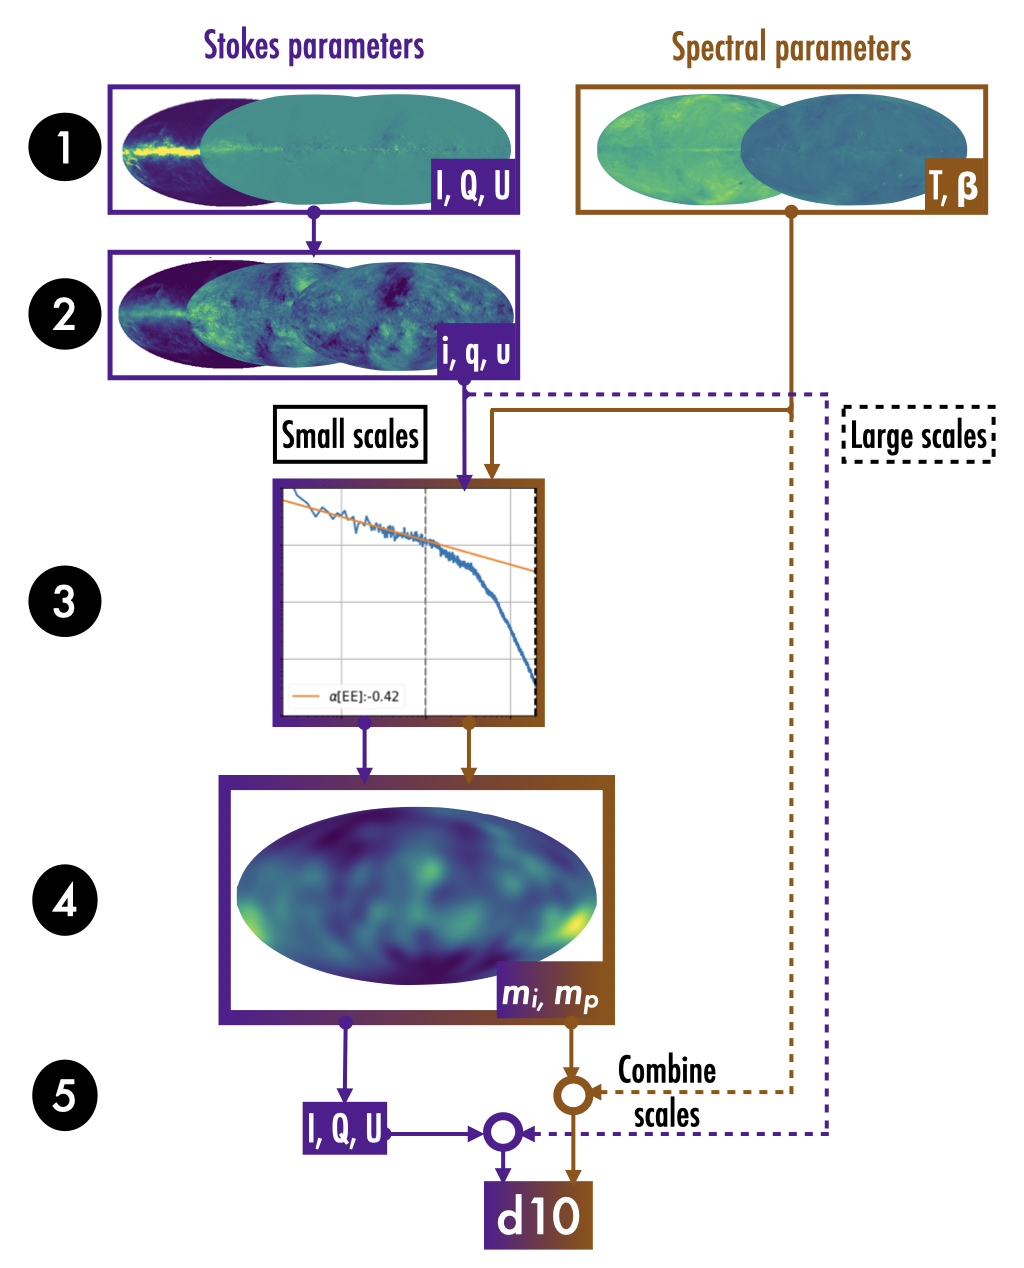
\includegraphics[width=\textwidth]{figures/draft_flowchart_fig_larger_scalesep2.001.jpeg}
    \caption{DRAFT flowchart figure}
    \label{fig:flowchart}
\end{figure*}
  
The adopted values of $\ell_1$ and $\ell_*$ are driven both by the angular resolution and the signal-to-noise ratio of the template maps. We employ $\ell_1=100$ and $\ell_*=80$ for dust and $\ell_1=38$ and $\ell_*=36$ for synchrotron. The $\ell_2$ parameter is chosen to be high enough that dust and synchrotron emission are relatively unconstrained by current full-sky data. We adopt  $\ell_2=2000$ for dust and $\ell_2 = 400$ for synchrotron. For dust we employ a power law index of $\alpha_{tt} = -0.80$ based on the range of fit $\alpha_{TT}$ in Planck, WISE, and MegaCam data by \citet{Miville-Deschenes:2016}. We adopt $\alpha_{ee} = -0.42$, $\alpha_{te} = -0.50$, and $\alpha_{bb} = -0.54$ from fits to Planck $TT$, $TE$, and $BB$ spectra, respectively, over 71\% of the sky \citep{planck2016-l11A}. For synchrotron we adopt $\alpha_{tt} = -1.00$ and $\alpha_{te} = -1.00$ based on the observed spectra of the synchrotron template map. We adopt $\alpha_{ee} = -0.84$ and $\alpha_{bb} = -0.76$ following fits to synchrotron maps over 78\% of the sky produced with the \texttt{Commander} pipeline \citep{planck2016-l04}. The $\ell_1$, $\ell_2$, $\ell_*$, and $\alpha$ values used to construct the small-scale maps are all summarized in Table~\ref{tab:smallscale_par}.

The final maps are obtained by combining the large and small scales: 
\begin{equation} \label{eq:filter}
    a_{\ell m }^{X, out}=  a_{\ell m }^{X, \mathcal{T}} \left(1-\sigma_\ell\right)^{\gamma} + a_{\ell m }^{X, ss} \sigma_\ell
    ~~~, 
\end{equation}
where $a_{\ell m }^{X, \mathcal{T}}$ are the coefficients of the large-scale templates, with $X$ any of $t$, $e$, and $b$, and $a_{\ell m }^{X, ss}$ is derived from the synthesized small-scale fluctuation maps. The exponent of $0.2$ on the $\left(1-\sigma_\ell\right)$ term is chosen empirically to smooth the transition between our data-driven templates and the generated small scales. We found that this choice minimizes artifacts at $\ell \simeq \ell_1$ in power spectra computed over large sky areas while maintaining the correct asymptotic behavior. The filter $\sigma_\ell$ is given by

\begin{equation} \label{eq:filter2}
\sigma_\ell  = \left[1+  e^{ -c_1 (\ell/ \ell_1  -c_2 )}\right]^{-1}  
~~~,
\end{equation}
where the parameters $c_1$ and $c_2$ govern the width of the filter in multipoles. We adopt $c_1=40$ and $c_2=1.05$ throughout this work.

Since the generation of the small scales depends only upon a fixed input power spectrum, we can generate a different map realization on the fly each time a sky is simulated. Thus, the methodology presented here enables generation of an ensemble of sky realizations having the same well-measured large scales but stochastic realizations of the poorly-measured small scales. Further, the small-scale fluctuations can be generated at arbitrarily small scales set only by the resolution of the map since all power spectra can be extended indefinitely in $\ell$. In practice, small scales are generated up to $\ell_{\rm max} = 3N_{\rm side}-1$.

We do not intend for the above procedure to be useful for the inner Galactic plane, which has been imaged at high signal-to-noise ratio at relatively small scales. We thus do not apply the small-scale amplitude extrapolation to the $3\%$ of the sky in the Galactic plane as defined by the Planck \texttt{GAL097} mask\footnote{\texttt{HFI\_Mask\_GalPlane-apo2\_2048\_R2.00.fits}}, where we instead use the observed templates as-is at all scales. To ensure a smooth transition between the template used in this region and synthesized small scales employed over the rest of the map, we apodize the mask with a $5^\circ$ Gaussian taper. This reflects our expectation that our procedure is most useful for making physically motivated synthetic realizations of diffuse Galactic emission at high Galactic latitudes rather than in the Galactic plane.

Another challenge for our prescription is pixels that, whether from noise or systematic errors, have $I^2 < P^2$, rendering the transformation in Equation~\eqref{eq:real2pt} invalid. We identify 527 such pixels in our dust template and 5 in our synchrotron template, all in the vicinity of the Crab Nebula. To address this, we set the $i$, $q$, and $u$ values at the location of these pixels to fiducial values of 4.51, 0.07, and 0.01 in the dust maps and 4.55, 0.017, $-0.001$ in the synchrotron maps. Given these complications, we do not advise using the simulations in the vicinity of the Crab Nebula.

Finally, we emphasize that our procedures are optimized for producing polarization rather than total intensity maps. For instance, we could in principle retain much smaller angular scales from the intensity templates, however we require uniform parameters in intensity and polarization to implement the polarization fraction tensor framework. Other choices, such as the value of $\gamma$, are based on polarization spectra. Some of the non-idealities of the maps in total intensity produced as a consequence of these choices are documented in Section~\ref{sec:validation}.

\subsubsection{Dust Amplitude}\label{sec:dustamplitude}
The Planck~2015 component separation results in total intensity remain state of the art despite updates in polarization in the 2018 data release \citep{planck2016-l04}. Previous PySM models, e.g., \texttt{d0} and \texttt{d1}, employed the dust templates from the \texttt{Commander} component separation analysis \citep{planck2014-a11}. However, the model fitting employed in \citet{planck2014-a11} did not differentiate between Galactic dust emission and the Cosmic Infrared Background (CIB), and so the component separated dust maps retain CIB signal that should not be included in simulations of Galactic emission (see Section~\ref{sec:CIBcontamination} for a detailed discussion). To address this issue, we instead use dust templates from analyses that separated Galactic dust emission from the CIB using the Generalized Needlet Internal Linear Combination (GNILC) algorithm \citep{Remazeilles:2011}. 

In total intensity we employ the Planck GNILC 2015 component separated map\footnote{\texttt{COM\_CompMap\_Dust-GNILC-F353\_2048\_R2.00.fits}} at $353$\,GHz \citep{planck2016-XLVIII}. This map has variable angular resolution, ranging from $21.8\arcmin$ up to $5\arcmin$ depending on the sky region, which complicates its use in our analysis. Therefore, we reprocess the map to a spatially uniform resolution of $21.8\arcmin$. To do so, we first note that the map was synthesized from ten needlet maps of different, but spatially-uniform, resolutions \citep[][Figure~A.2]{planck2016-XLVIII}. Each of the $j=1,\cdots,10$ needlet maps can be reconstructed from the Planck GNILC 2015 dust map as follows:

\begin{equation}
\gamma^{j}(\hat{n})
=\sum_{\substack{\ell,m}} \left(a_{\ell m}\, h^{j}_\ell\right)Y_{\ell m}(\hat{n})\,,
\label{eq:needlets_maps}
\end{equation}
where $a_{\ell m}$ are the spherical harmonic coefficients of the Planck GNILC 2015 dust map,  $h^{j}_\ell$ is the $j^\text{th}$ needlet window function \citep[see][Figure~A.2]{planck2016-XLVIII}, and $Y_{\ell m}(\hat{n})$ denotes spherical harmonics. We produce a map of uniform resolution by retaining only the first six needlet maps\footnote{Available at NERSC: \url{https://portal.nersc.gov/project/cmb/pysm-data/dust_gnilc/inputs/}}, which probe the dust intensity from the largest scales down to $21.8\arcmin$:

 \begin{equation}
 d^{\text{GNILC,}\, 21.8'}(\hat{n})
=\sum_{j=1}^6 h^{j}_\ell \gamma^{j}(\hat{n})\,.
\label{eq:trucated_synthesis}
\end{equation}
This yields an $N_{\rm side} = 2048$ map that reproduces the Planck GNILC 2015 dust intensity template at all scales $\geq 21.8\arcmin$. Finally, we subtract the CIB monopole of $0.13\, \text{MJy}\,\text{sr}^{-1}$ present in the map \citep[][Section~2.2]{planck2016-l11B}.

For the dust $Q$ and $U$ maps we employ the dust maps\footnote{\texttt{COM\_CompMap\_IQU-thermaldust-gnilc-varres\_2048\_R3.00.fits}} produced by the GNILC component separation from the Planck Public Release 3 \citep{planck2016-l04,planck2016-l11B}. While these maps have variable angular resolution, the resolution varies over the sky much more smoothly than in the $I$ map. Given this, and that we wish to retain as much polarization information in our analysis as possible, we employ these variable resolution maps as-is. Their resolution ranges from $5\arcmin$ in the Galactic plane to $80\arcmin$ at high Galactic latitudes. The maps are pixellated at $N_{\rm side} = 2048$. 

To produce dust emission templates at a monochromatic frequency of 353\,GHz, we divide each of the $I$, $Q$, and $U$ maps by a factor of 1.098 to correct for the Planck bandpass \citep[][Table~2]{planck2016-l11A}.

\subsubsection{Synchrotron Amplitude}
Deriving a full-sky template for synchrotron emission in total intensity is challenging both for the paucity of low frequency surveys with full sky coverage and the difficulty in disentangling synchrotron emission from free-free emission and AME at frequencies above $\sim$10\,GHz. We follow \citet{Thorne:2017} in basing our template on the Haslam 408\,MHz survey \citep{Haslam:1982} and in particular the reprocessing of the original maps by \citet{Remazeilles:2015}. We rescale the 408\,MHz map to 23\,GHz assuming a sky-constant scaling of the brightness temperature with $\nu^{-3.1}$. Finally, we smooth the resulting map with a $2^\circ$ Gaussian beam.

A key limitation of the current synchrotron total intensity template is that, despite the point source masking, we still find excess power from Galactic point sources at low Galactic latitudes near the Galactic center. Our models are unaffected by this issue at $\ell \lesssim 3000$ and outside the Galactic plane. Addressing small scale structures in bright regions will be deferred to a future release.

Constructing a synchrotron template in polarization is somewhat easier than total intensity because both free-free emission and AME have very low levels of polarization. Thus, we directly employ the WMAP K-band (23\,GHz) $Q$ and $U$ maps\footnote{\url{https://lambda.gsfc.nasa.gov/data/map/dr5/skymaps/9yr/raw/wmap_band_iqumap_r9_9yr_K_v5.fits}} from Data Release~5 directly as our templates. As with the $I$ map, we smooth the $Q$ and $U$ templates with a $2^\circ$ Gaussian beam.

\subsection{Small Scale Fluctuations in Spectral Parameters} \label{sec:spec_params}

\subsubsection{Methods Overview} \label{subsec:spec_params_overview}

\begin{deluxetable}{lccc}
    \caption{Model parameters for synthesizing spectral parameter maps at small scales}
   \tablehead{& \colhead{$\ell_0$} & \colhead{$\ell_1$} & \colhead{$\alpha$}}
   \startdata
   $\beta_d$ & 200 & 400 & 0.04 \\ 
   $T_d$ & 100 & 400  & -0.47\\
    $\beta_s$ & 10 & 36 & -0.61\\
    $c_s$ & 10 & 36 & -0.61  \\ 
    \enddata
    \tablecomments{Spectra are parameterized assuming $\mathcal{D}_\ell^{XX} \propto \ell^{\alpha_{XX}}$.}
    \label{tab:smallscale_specpar}
\end{deluxetable}

Just as a map of Galactic emission at a single frequency is expected to have fluctuations at smaller angular scales than have been measured, maps of parameters governing its frequency dependence should also have small-scale fluctuations. We therefore introduce small scale fluctuations to our spectral parameter template maps in a way analogous to the amplitude template maps. This more realistically captures the complexity of small-scale Galactic emission.

As there is no sense of polarization in the spectral parameter maps, we do not work within the polarization fraction tensor framework but rather with standard power spectra. Given a template map $\mathcal{T}$ of some spectral parameter $X$, we first fit the power spectrum of $\mathcal{T}$ with a power law $\mathcal{D}_\ell^{XX} \propto \ell^\alpha$ over a range of scales $\ell_0 < \ell < \ell_1$ where it is well measured. We then generate a map of small scale fluctuations using the power law fit. We multiply the resulting map by a modulation map in analogy with the amplitude modulations described in Section~\ref{subsec:methodology}. Finally, we combine the template map with the synthesized small scales using the filter function in Equation~\ref{eq:filter}. As with the amplitude parameters, we use the input template maps for the spectral parameters as-is in the inner Galactic plane, defined by the Planck \texttt{GAL097} mask.

An important caveat with introducing random fluctuations in the spectral parameters is that the resulting emission maps are no longer guaranteed to resemble data far from the reference frequency. For this reason, we recommend that models with variations in spectral parameters be used only in the frequency range $\sim$1--1000\,GHz.

The application of this procedure to the dust and synchrotron spectral parameters is described in the following sections. The adopted fit parameters for each spectral parameter are listed in Table~\ref{tab:smallscale_specpar}.

\subsubsection{Dust Spectral Parameters}\label{subsec:dust_spec_params}
As described in Section~\ref{subsubsec:dust_model}, the dust emission in all models developed here is governed by the spectral parameters $\beta_d$ and $T_d$. For the $\beta_d$ and $T_d$ template maps, we employ the $\beta_d$ and $T_d$ maps\footnote{\texttt{COM\_CompMap\_Dust-GNILC-Model-Spectral-Index\_2048\_R2.00.fits}, \texttt{COM\_CompMap\_Dust-GNILC-Model-Temperature\_2048\_R2.00.fits}} derived from 2015 Planck GNILC component separation analysis \citep{planck2016-XLVIII}. These maps have lower CIB contamination than the \texttt{Commander} $\beta_d$ and $T_d$ maps \citep{planck2014-a12} as the methodology employed both spatial and spectral information to disentangle the CIB contribution to the total emission (see discussion in Section~\ref{sec:CIBcontamination}).
%However, the estimate of $\beta_d$ and $T_d$ is highly degenerate making the maps at small angular scales ($<21.8^\prime$) are contaminated by artifacts due to noise and calibration errors. 

We fit the power spectra of the $\beta_d$ and $T_d$ template maps over the multipole ranges $200 < \ell < 400$ and $100 < \ell < 400$, respectively. We find that $\alpha_{\beta_d}= 0.04$ and $\alpha_{T_d} = -0.47$ over this range, both flatter than the $\alpha_{tt} = -0.80$ found for the dust amplitude. The adopted pivot multipole $\ell_1$ is larger than that used for dust amplitudes (see Table~\ref{tab:smallscale_par}) since the template maps employed here are derived from intensity-only data rather than a combination of total and polarized intensity. Thus, they remain signal-dominated at $\sim$4 times smaller angular scales. We employ the same modulation map as was used for the dust amplitude (see Section~\ref{subsec:methodology}).

\subsubsection{Synchrotron Spectral Parameters}\label{sec:beta_s}
As described in Section~\ref{subsubsec:synch_model}, the synchrotron emission in all models developed here is governed by the spectral parameters $\beta_s$ and $c_s$. To build the large scale template for the spatial variation of the synchrotron spectral index $\beta_s$, we begin with the full-sky $\beta_s$ map of \citet{Miville-Deschenes:2008} obtained by combining the Haslam map in total intensity at 408\,MHz \citep{Remazeilles:2015} and WMAP 3\,yr K-band data \citep{Hinshaw:2007}. The map has an angular resolution of about $7^{\circ}$ and was employed by previous PySM synchrotron models \citep{Thorne:2017}.

Incorporating newer constraints on synchrotron emission at 2.3\,GHz from S-PASS, \citet{Krachmalnicoff:2018} determined that this $\beta_s$ map underestimates the true level of spatial variations in $\beta_s$ across the Southern Galactic Hemisphere. Thus, we follow \citet{Krachmalnicoff:2018} and rescale the $\beta_s$ map by first subtracting its mean value ($\bar{\beta} = -3.00$), multiplying the resulting map by a factor of $1.572$, and then adding back the mean value.

We next fit a power-law to the power spectrum of this new template map over the multipole range $10 < \ell < 36$, finding $\alpha_{\beta_s}=-0.61$ then construct a map from this power spectrum extrapolated to high multipoles. The $\beta_s$ small scales are modulated employing the same modulation map as the synchrotron intensity map (see Section~\ref{subsec:methodology}). As with the dust spectral parameter maps (see Section~\ref{subsec:dust_spec_params}), we combine this high-$\ell$ map with the low-$\ell$ template following the filter function of Equation~\ref{eq:filter}.
 
For the synchrotron curvature parameter $c_s$, there are no readily available template maps. The existing \texttt{s3} model implements curvature as a sky-constant $c_s = -0.052$, consistent with the measurements from ARCADE \citep[$c_s=-0.052 \pm 0.005$,][]{Kogut:2012}. To model a reasonable range of spatial variability, we assume that fluctuations in the value of $c_s$ follow the synchrotron intensity at large angular scales. Specifically, we start from the Haslam map 408\,MHz $I$ map of \citet{Remazeilles:2015} smoothed to a resolution of $5 \deg$. We then rescale this map with a linear transformation such that the minimum and maximum pixel values over the full sky are $-0.076$ and $-0.041$ respectively, corresponding to the approximate range of $c_s$ measurements from ARCADE \citep[][Figure~6]{Kogut:2012}. The resulting $c_s$ map has a mean and standard deviation of $-0.0517$ and $0.0054$, respectively, within the ARCADE footprint, in good agreement with the ARCADE measurements.

To extend our $c_s$ map to angular scales $\ell > \ell_1 = 36$, we first generate a map of Gaussian random fluctuations with the same power law index as the $\beta_s$ map, i.e., $\alpha _{c_s}=\alpha _{\beta_s} = -0.61$. We modulate the resulting map with the Haslam 408\,GHz $I$ map, smoothed to $5^\circ$ FWHM resolution. We renormalize the map through a linear transformation such that the (dimensionless) pixel values range from 0.1--2. Finally, the modulated high-$\ell$ map is combined with the low-$\ell$ template following the filter function of Equation~\ref{eq:filter}.

\subsection{Summary of New Dust and Synchrotron Models}

The new dust and synchrotron models implemented here all improve on previous models through new data-driven templates and use of the polarization fraction tensor framework to model small-scale fluctuations. Multiple models of dust and synchrotron are provided to explore a range of astrophysical complexity allowed by current constraints. In brief, the \texttt{d9} and \texttt{s4} models use the new data-driven templates and include $I$, $Q$, and $U$ fluctuations up to the largest $\ell$ values simulated, but these models have sky-constant spectral parameters and thus no frequency decorrelation (see Section~\ref{subsec:decorrelation} for discussion). In contrast, \texttt{d10} and \texttt{s5} employ data-driven maps of spectral parameters to which small-scale fluctuations are added, inducing frequency decorrelation. The \texttt{s7} synchrotron model provides an extra spectral parameter---curvature of the frequency spectrum---and thus additional complexity. The \texttt{d11} and \texttt{s6} models allow many realizations of \texttt{d10} and \texttt{s5}, respectively, to be generated in which the large scales are fixed to the data-driven templates and the small scales have the same statistical properties but differing spatial morphologies. Tables~\ref{table:summarydust} and \ref{table:summarysynch} provide a high-level summary of these models. Extensive model comparisons are made in Section~\ref{sec:validation}.

\section{Other Models Implemented} \label{sec:other_models}

\subsection{Dust Layer Model} \label{sec:layers}
Evidence for variation of Galactic foreground emission laws as a function of frequency across the sky \citep[e.g.,][]{Krachmalnicoff:2018, SPIDERCollaboration:2024} implies that emission laws must also vary along the line of sight. As a consequence, even if dust emission can be described locally by a modified blackbody (Equation~\ref{eq:dust-emission-law}), a superposition of emission regions (i.e., an integral along the line of sight) is not a modified blackbody. In addition, if along the line of sight different line elements emit polarized radiation with different polarization angles, the frequency scaling can vary between $I$, $Q$ and $U$ \citep{Tassis:2015}. Evidence for this ``line-of-sight frequency decorrelation'' has been found in Planck data \citep{Pelgrims:2021}.

To model the complexity of multiple layers of dust along the line of sight, we base our PySM~3 implementation \texttt{d12} on the approach of \cite{Martinez-Solaeche:2018} in the PSM software\footnote{See version 2.3.3 \url{https://apc.u-paris.fr/~delabrou/PSM/psm.html}.}. 

The PSM has been run to produce six maps of dust emission $S_{\nu_0}^k(\theta)$ at $\nu_0 = 353$ GHz (intensity and polarization, for a total of 18 HEALPix maps at $N_{\rm side}$=2048), and six maps of dust spectral index $\beta_d^k(\theta)$ and dust temperature $T_d^k(\theta)$ at $N_{\rm side}$=2048, following the approach described in \cite{Martinez-Solaeche:2018}, to form six different layers.

The PySM software uses these maps as inputs, and generates the dust Stokes parameters maps as:
\begin{equation}
    S_\nu(\theta) = \sum_{k=1}^6 S^{(k)}_{\nu_0}(\theta)
    \left( \frac{\nu}{\nu_0} \right)^{\beta^{(k)}_d(\theta)}
    \frac{B_\nu(T^{(k)}_d(\theta))}{B_{\nu_0}(T^{(k)}_d(\theta))},
\end{equation}
where $S_\nu(\theta)$ stands for any of the three Stokes parameters of interest, $I$, $Q$ and $U$, at frequency $\nu$ at sky location $\theta$, and superscripts ${(k)}$ indicate the layer, from one to six.

In the implementation used here, the 353~GHz templates for the six emission layers are slightly different from those of \cite{Martinez-Solaeche:2018}. They are generated at Healpix $N_{\rm side} = 2048$ instead of 512, with a revised version of the pipeline. Intensity maps are based on the Planck PR2 GNILC maps, while large scale polarized emission maps are the GNILC maps obtained in \cite{Martinez-Solaeche:2018}. These are complemented by small scale realizations with scale dependence matching the $I$, $E$ and $B$ dust spectra measured in \cite{planck2016-l11A}, modulated by the large scale local intensity and polarized intensity level. Specifically, for each layer $k$, and for each of $T$, $E$ and $B$, we model the final emission in harmonic space as:
\begin{equation}
    S^{(k)}_{\nu_0} = X^{(k)}_{\nu_0} h_\ell^{1/2} + Y^{(k)}_{\nu_0} (1-h_\ell)^{1/2},
\end{equation}
where $X^{(k)}_{\nu_0}$ is the observed emission deconvolved from the instrumental beam, $Y^{(k)}_{\nu_0}$ is a randomly generated set of harmonic coefficients with harmonic spectrum following Planck constraints \citep{planck2016-l11A}, and $h_\ell$ is a window defining the transition between the two regimes. For intensity, $h_\ell$ corresponds to a $5\arcmin$ beam window function, while for polarization, we use a $150\arcmin$ beam for the three nearest layers (which dominate at high Galactic latitude) and a $120\arcmin$ beam for the three farthest layers (which dominate near and in the Galactic plane).

The construction of these maps does result in some filtering out of the real small scale power in intensity and polarization, which is replaced by random fluctuations. Thus we expect departures from the non-Gaussian and non-stationary properties of real dust emission at these scales.

In this model, maps of spectral parameters ($\beta_d$ and $T_d$) are randomly generated for each layer as described in \cite{Martinez-Solaeche:2018}. As a consequence, they are not constrained to match the observed temperature and spectral index maps. While their statistics (e.g., amplitude, correlation between $\beta_d$ and $T_d$) are compatible with those of real data, they provide a different realization, which results in increased differences between the real sky and the model at frequencies increasingly far from the reference frequency, $\nu_0 = 353$~GHz.

\subsection{CO Models} \label{subsec:co_models}
Galactic CO line emission is strong enough that the $J = 1\rightarrow0$, $J = 2\rightarrow1$, $J = 3\rightarrow2$ transitions have been detected even in the broad photometric Planck bands \citep{planck2013-p03a, planck2014-a12}. CO emission can be polarized \citep{Goldreich:1981} and so is a relevant foreground for CMB polarization analyses \citep{Puglisi:2017}. In this section, we describe the implementation of three CO models into the PySM~3 framework.

Because of the intrinsically low degree of CO polarization and the long integration time required to achieve a significant detection, it is difficult to carry out CO polarization surveys and wide area measurements have not yet been made. In the absence of data-based templates, the approach to modeling CO has been to assume a small degree of polarization applied to total intensity maps. For instance, \citet{Puglisi:2017} presented a model to simulate the polarized emission of CO lines in molecular clouds at high Galactic latitudes by considering the 3D spatial distribution of CO in the Galaxy.

All CO models implemented here are based on the CO $J = 1\rightarrow0$, $J = 2\rightarrow1$, $J = 3\rightarrow2$ \texttt{Type-1} intensity maps\footnote{\url{HFI_CompMap_CO-Type1_2048_R2.00.fits}} derived by \citet{planck2013-p03a} from Planck data. The CO maps are obtained exploiting the mismatches in the detector bandpasses to recover the CO from the CMB and the other Galactic foregrounds using the Modified Internal Linear Combination Algorithm (\texttt{MILCA}). The templates produced from this analysis are preferred to direct measurements from existing spectroscopic surveys \citep[e.g.,][]{Dame:2001} because they are not limited to low Galactic latitudes and have a uniform angular resolution over the sky.

\citet{planck2013-p03a} also produced \texttt{Type-2} templates based on a multi-frequency analysis. However, this method is more prone to modeling errors in separating the Galactic dust emission from the CO emission, and so we prefer the \texttt{Type-1} templates for our purposes.

The \texttt{Type-1} CO templates have a native resolution of $10\arcmin$. We convolve each of the $J = 1\rightarrow0$, $J = 2\rightarrow1$, and $J = 3\rightarrow2$ maps with a 1$^\circ$ Gaussian beam to reduce noise contamination, especially at intermediate and high Galactic latitudes, at the possible expense of introducing residual emission from extended Galactic and extra-galactic sources. Finally, the templates are downgraded to a coarser pixellization of $N_{\rm side} = 512$. These templates are the foundation on which all three of the CO models are built.

The first CO model \texttt{co1} adopts the $J = 1\rightarrow0,$  $J = 2\rightarrow1$ and $J = 3\rightarrow2$ templates as-is and assumes no polarization. 

The second CO model \texttt{co2} introduces a simple implementation of polarization. The $I$ maps of the three transitions used in \texttt{co1} are converted to $P$ maps using a sky-constant, user-defined polarization fraction $p$, where the default is $p = 0.1$\%. The $Q$ and $U$ maps are made from the $P$ maps using the polarization angle of the thermal dust emission as determined by a component separation analysis with Commander \citep{planck2014-a12}.

Finally, the third CO model \texttt{co3} not only accounts for the polarized emission as in \texttt{co2} but also includes small-scale emission from high-Galactic latitude clouds. We perform a dedicated simulation with the {\bf\texttt{LogSpiral}} model from \citet{Puglisi:2017}, which provided the best fit to Planck data, to produce maps of the contribution to the total and polarized CO intensity at sub-degree scales from molecular clouds at high Galactic latitudes. The $I$, $Q$, and $U$ maps generated by the simulation are then added to the $I$, $Q$, and $U$ maps of \texttt{co2} to produce the final \texttt{co3} model. This injection introduces CO emission at scales $\lesssim1^\circ$ in regions where the CO templates have very low signal-to-noise ratio. 

 
\section{Validation and Characterization of Models} \label{sec:validation}

In this section, we compare the new foreground models presented in this worth both to data and to previous models. In Section~\ref{subsec:maps}, map-based comparisons are made to visually highlight differences between the models and observational data. In Section~\ref{sec:PS-validation}, we compare power spectra of the dust and synchrotron models with observations. After developing the methodology in Section~\ref{subsubsec:methods}, we demonstrate that the two-point statistics of the stochastic small scales are properly modulated for different regions of sky defined by Galactic masks of varying size. Section~\ref{sec:dust_validation} compares the dust models to Planck NPIPE maps at 353\,GHz. Section~\ref{sec:sync_validation} compares the PySM synchrotron models with the synchrotron map from the BeyondPlanck analysis for intensity, and with the Planck Revisited reprocessed maps for polarization. Additional validation is performed in the sky patch observed by the BICEP/Keck telescopes in Section~\ref{sec:BK_validation}. Section~\ref{subsec:decorrelation} compares the level of frequency decorrelation in dust $BB$ emission across the models, demonstrating that all models respect current constraints from Planck observations. Section~\ref{sec:CIBcontamination} quantifies the level of extragalactic contamination in the maps. In Section~\ref{sec:nongaussianity}, we assess the level of non-Gaussianity introduced by the polarization fraction tensor formalism.

Since the \texttt{d10} model is one particular realization of the stochastic model \texttt{d11}, and likewise \texttt{s5} is one realization of \texttt{s6}, all comparisons presented here are performed using \texttt{d10} and \texttt{s5}. We find that other realizations of \texttt{d11} and \texttt{s6} produce qualitatively consistent results.

\subsection{Maps}\label{subsec:maps}

We provide several map-level comparisons between PySM dust models and observations. Specifically, we compare data from the Planck third data release PR3 \cite{planck2016-l03} and PySM dust models \texttt{d1} (which was widely used as a reference in previous versions of the PySM, and is described in \cite{Thorne:2017}), {\tt d9} (which is similar to \texttt{d1}, but uses different input templates and includes small scale fluctuations of template maps and spectral parameters, as described in Sec.~\ref{sec:small_scales}), and {\tt d12}, which is conceptually quite different from the other two models. The goal is to provide a qualitative comparison of the spatial characteristics of the models at small scales. We select $16.7^\circ \times 16.7^\circ$ patches of the sky, and compare the data and models at 353~GHz in both total and polarized intensity. We focus on two patches, one close to the Galactic plane with $(l,b) =(180^\circ,-10^\circ)$, and the second centered on the BICEP/Keck field at $(l,b) =(318^\circ,-61^\circ)$. 

\begin{figure*}[t!]
    \centering
    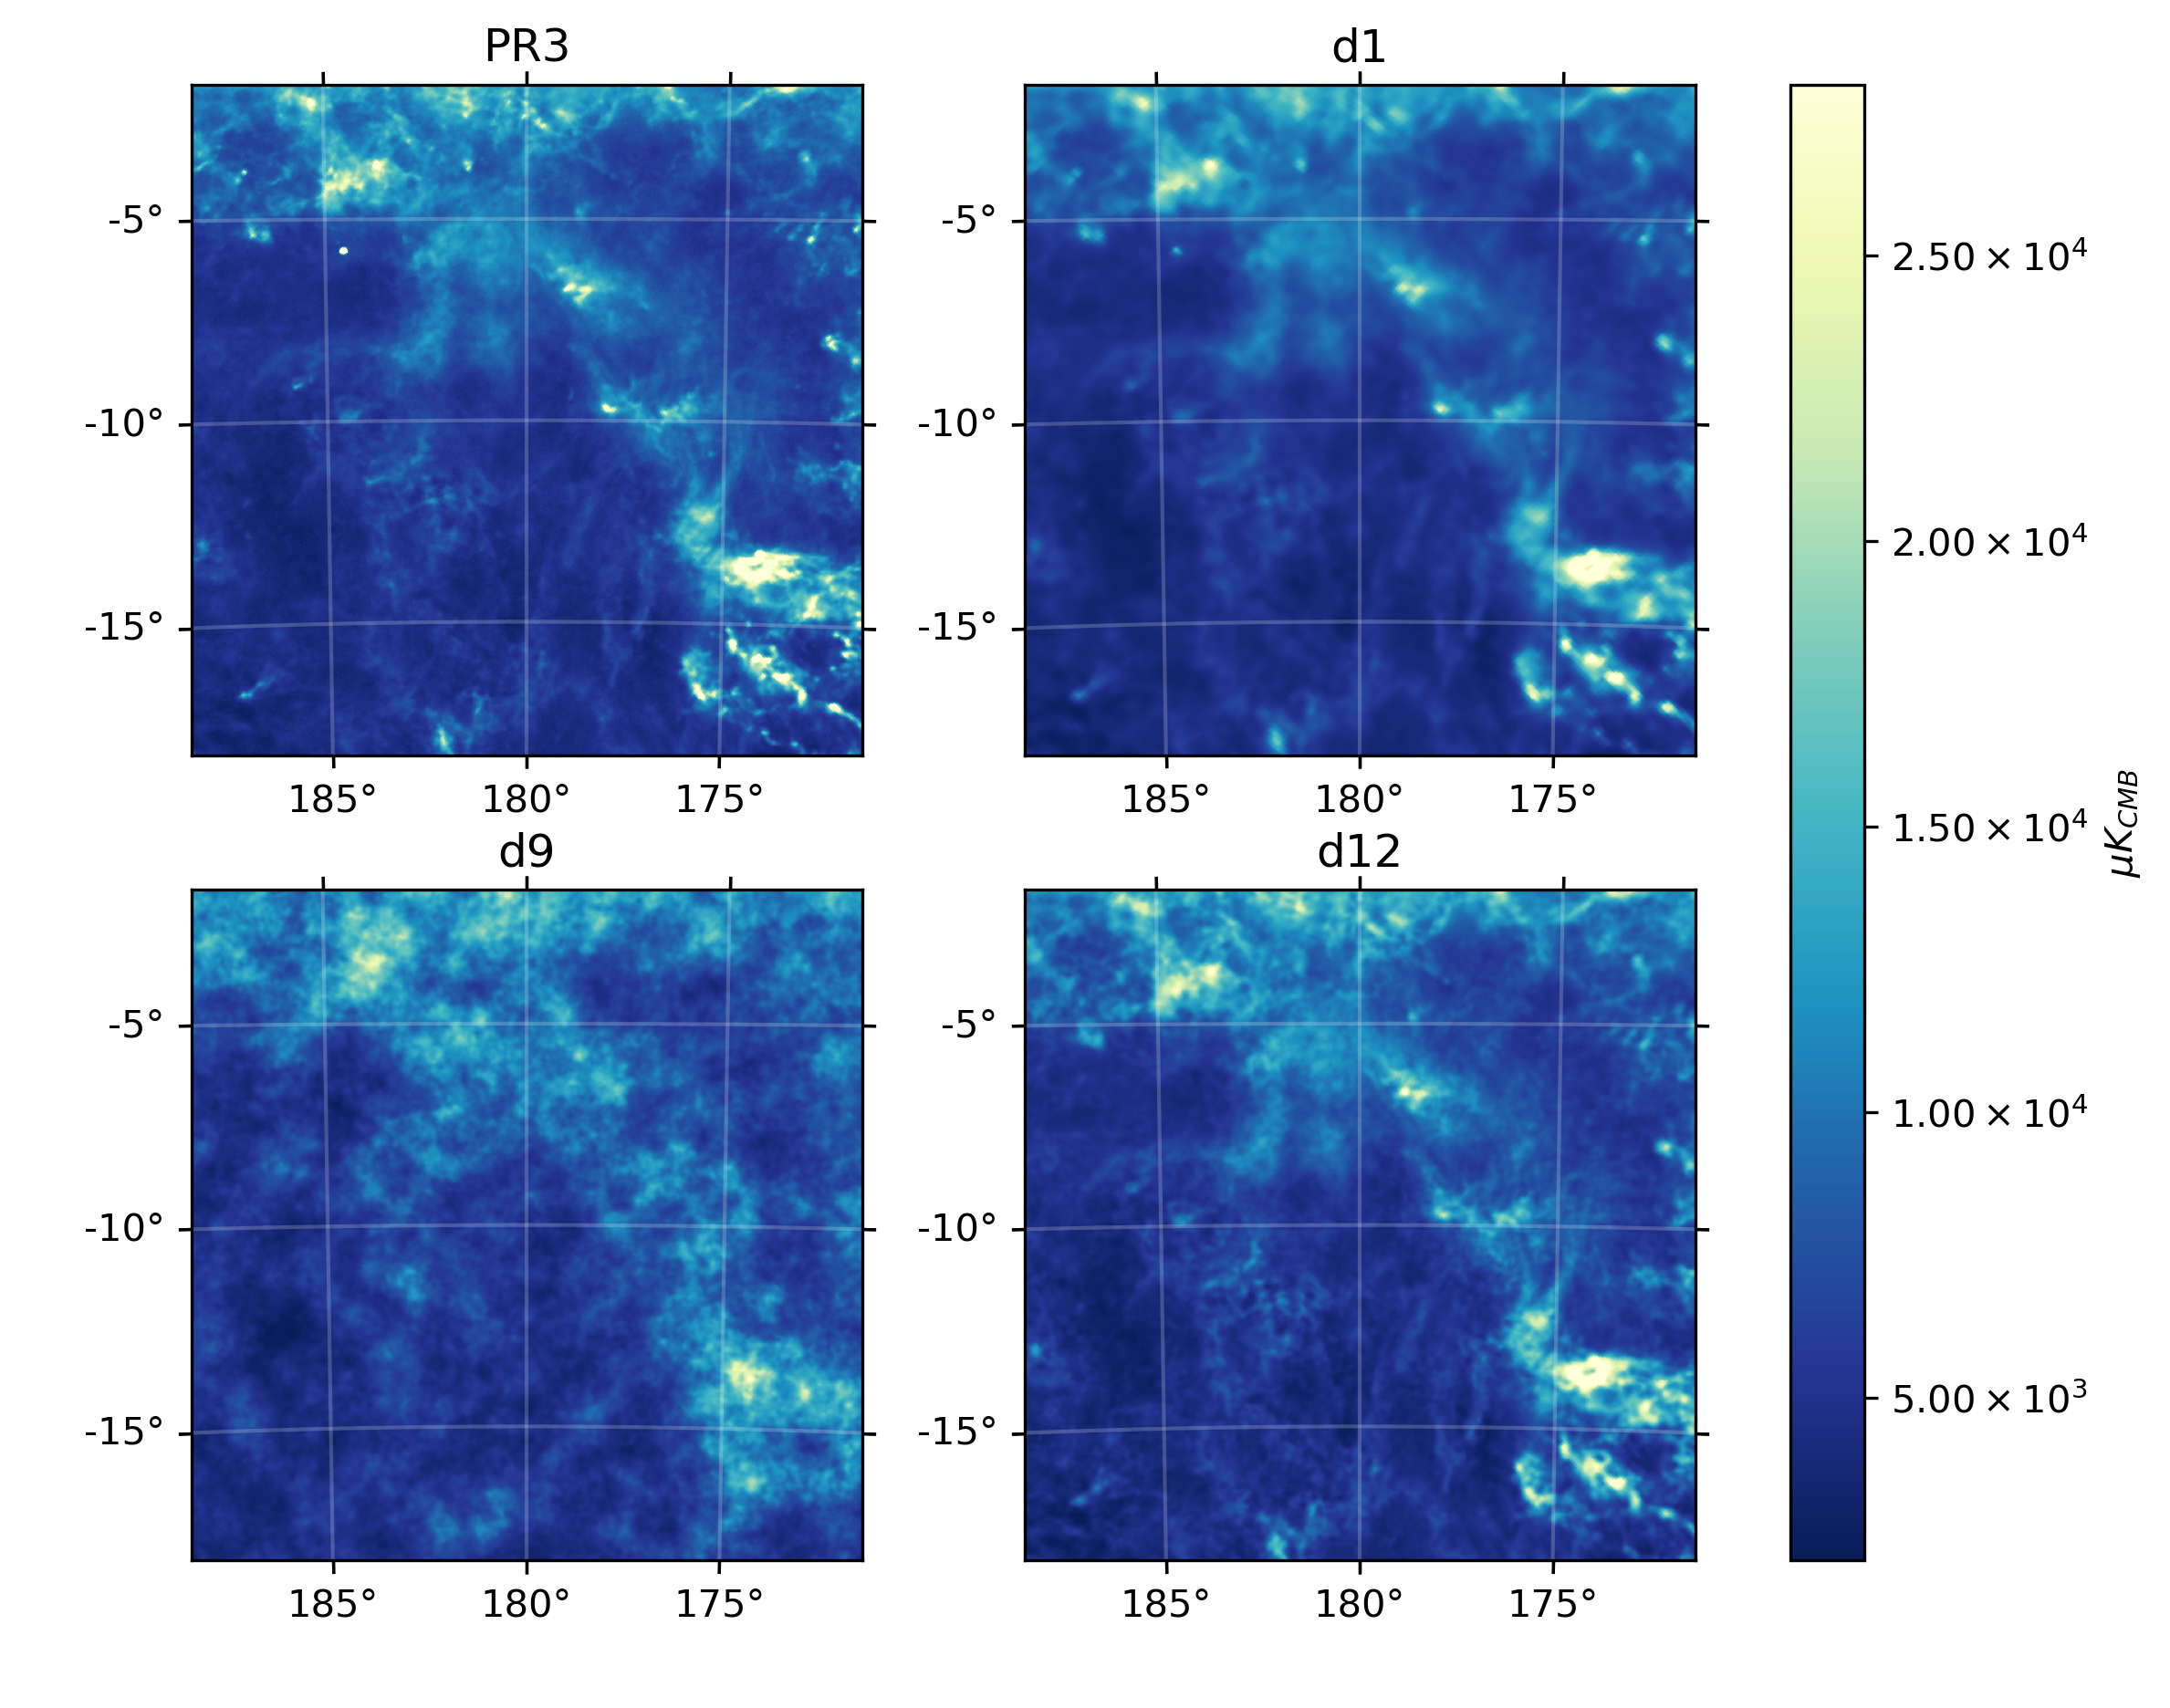
\includegraphics[height=0.395\textwidth]{figures/I_gal_plane.png}
    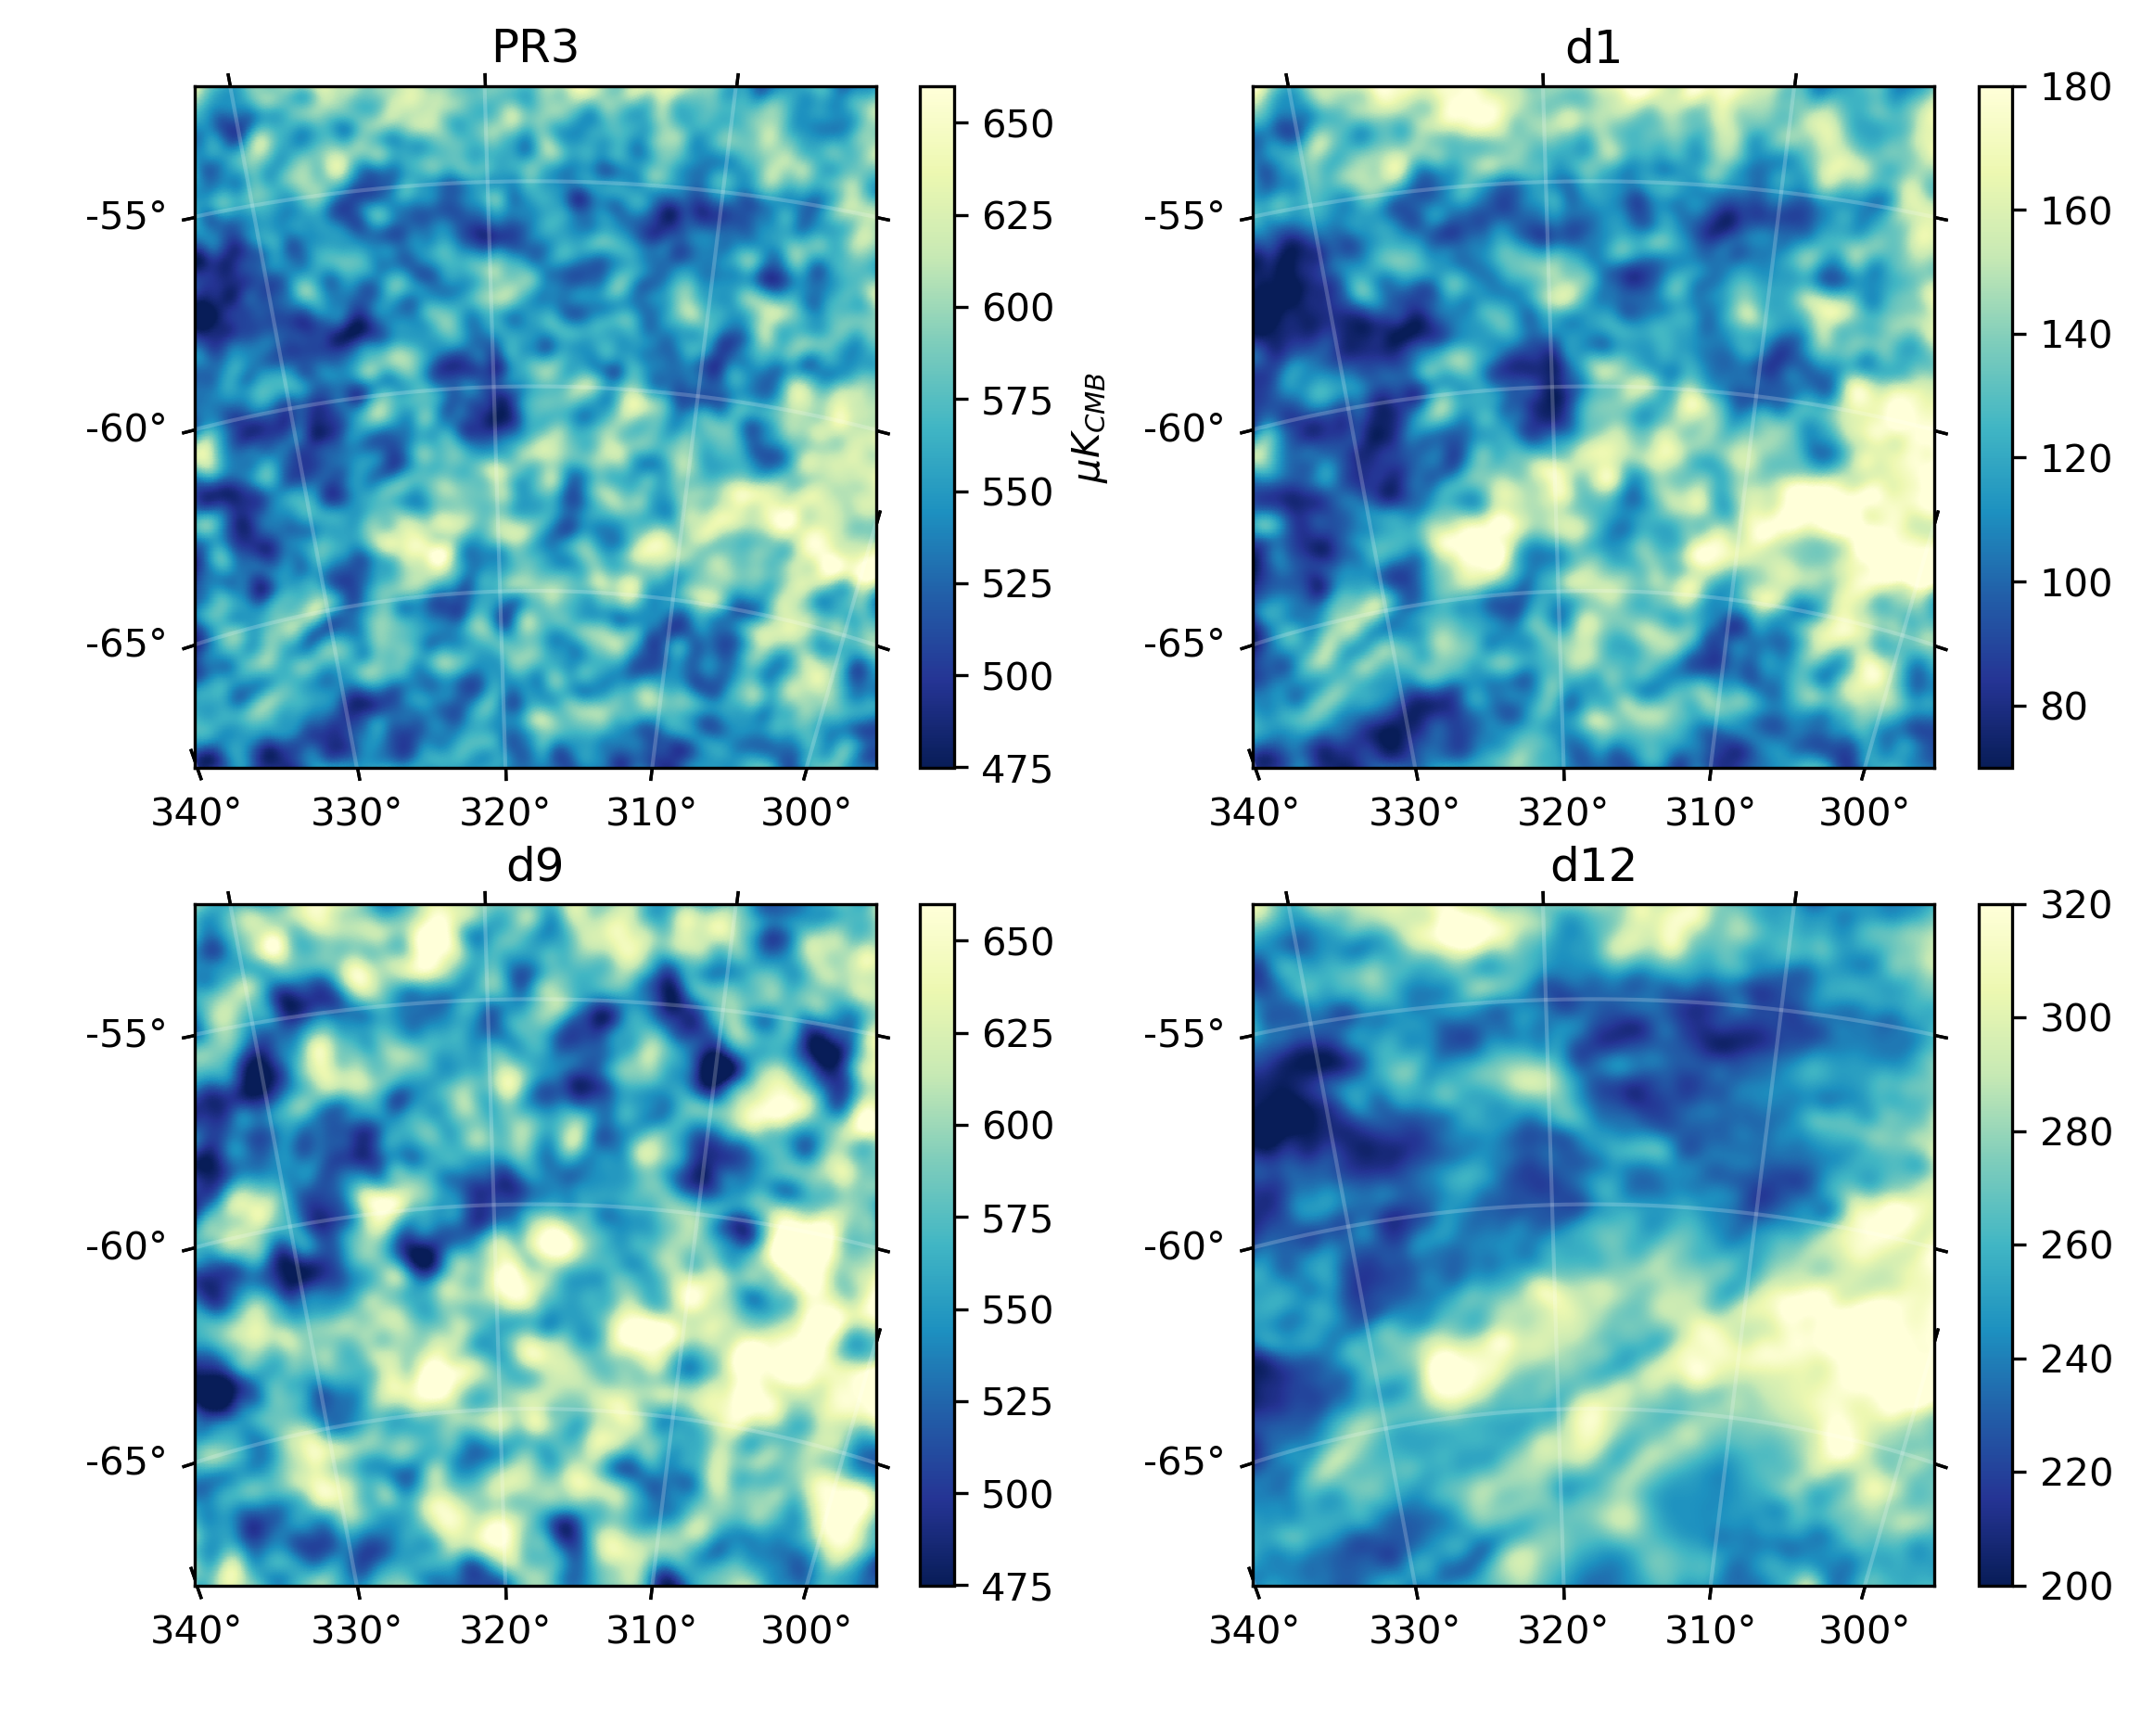
\includegraphics[height=0.395\textwidth]{figures/I_BK.png}
\caption{Dust intensity at 353GHz at [l = 180, b = -10] (left) and [l = 318, b = -61] (right) with an angular resolution of $4.94\arcmin$.}    
\label{fig:353_int}
\end{figure*}

\begin{figure*}[t!]
    \centering
    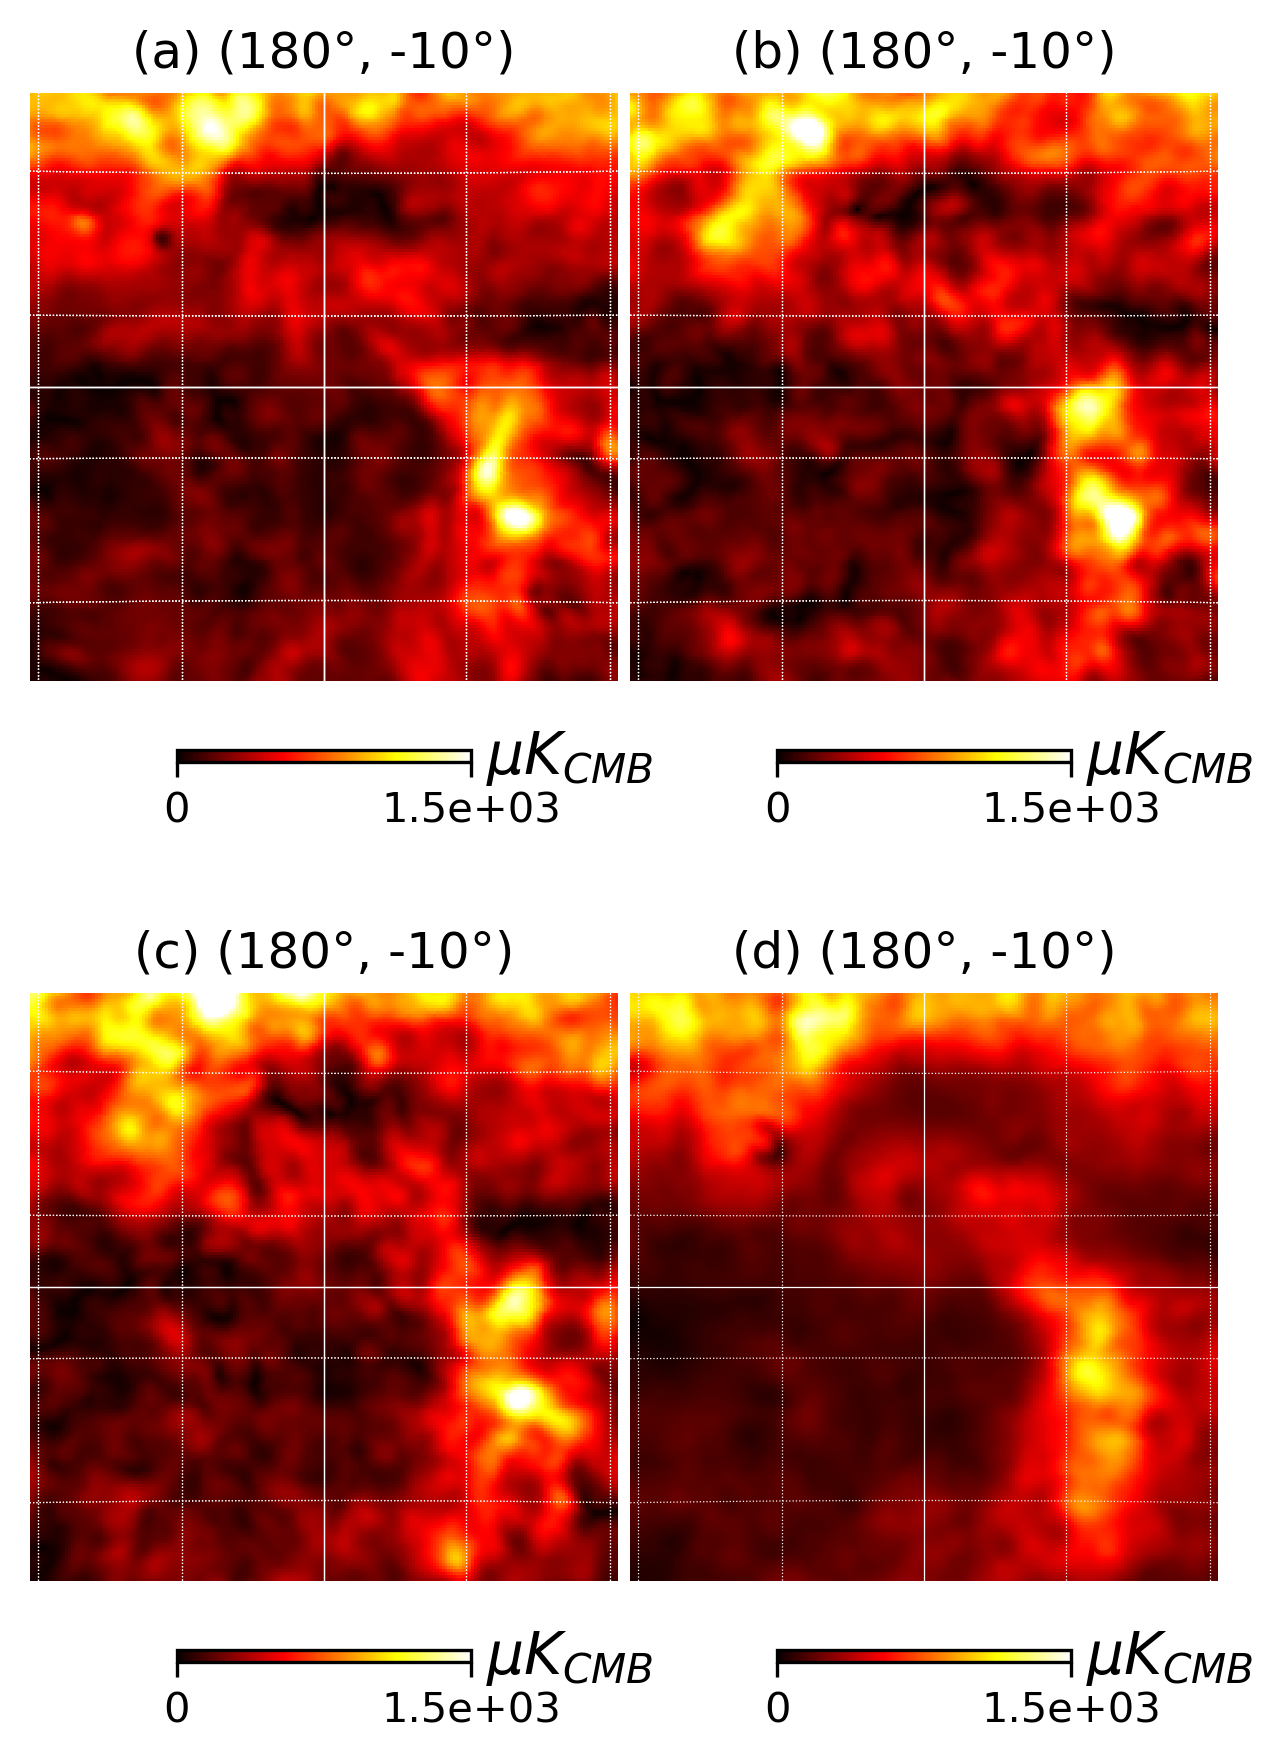
\includegraphics[height=0.41\textwidth]{figures/pol_gal_plane_smooth_30'.png}
    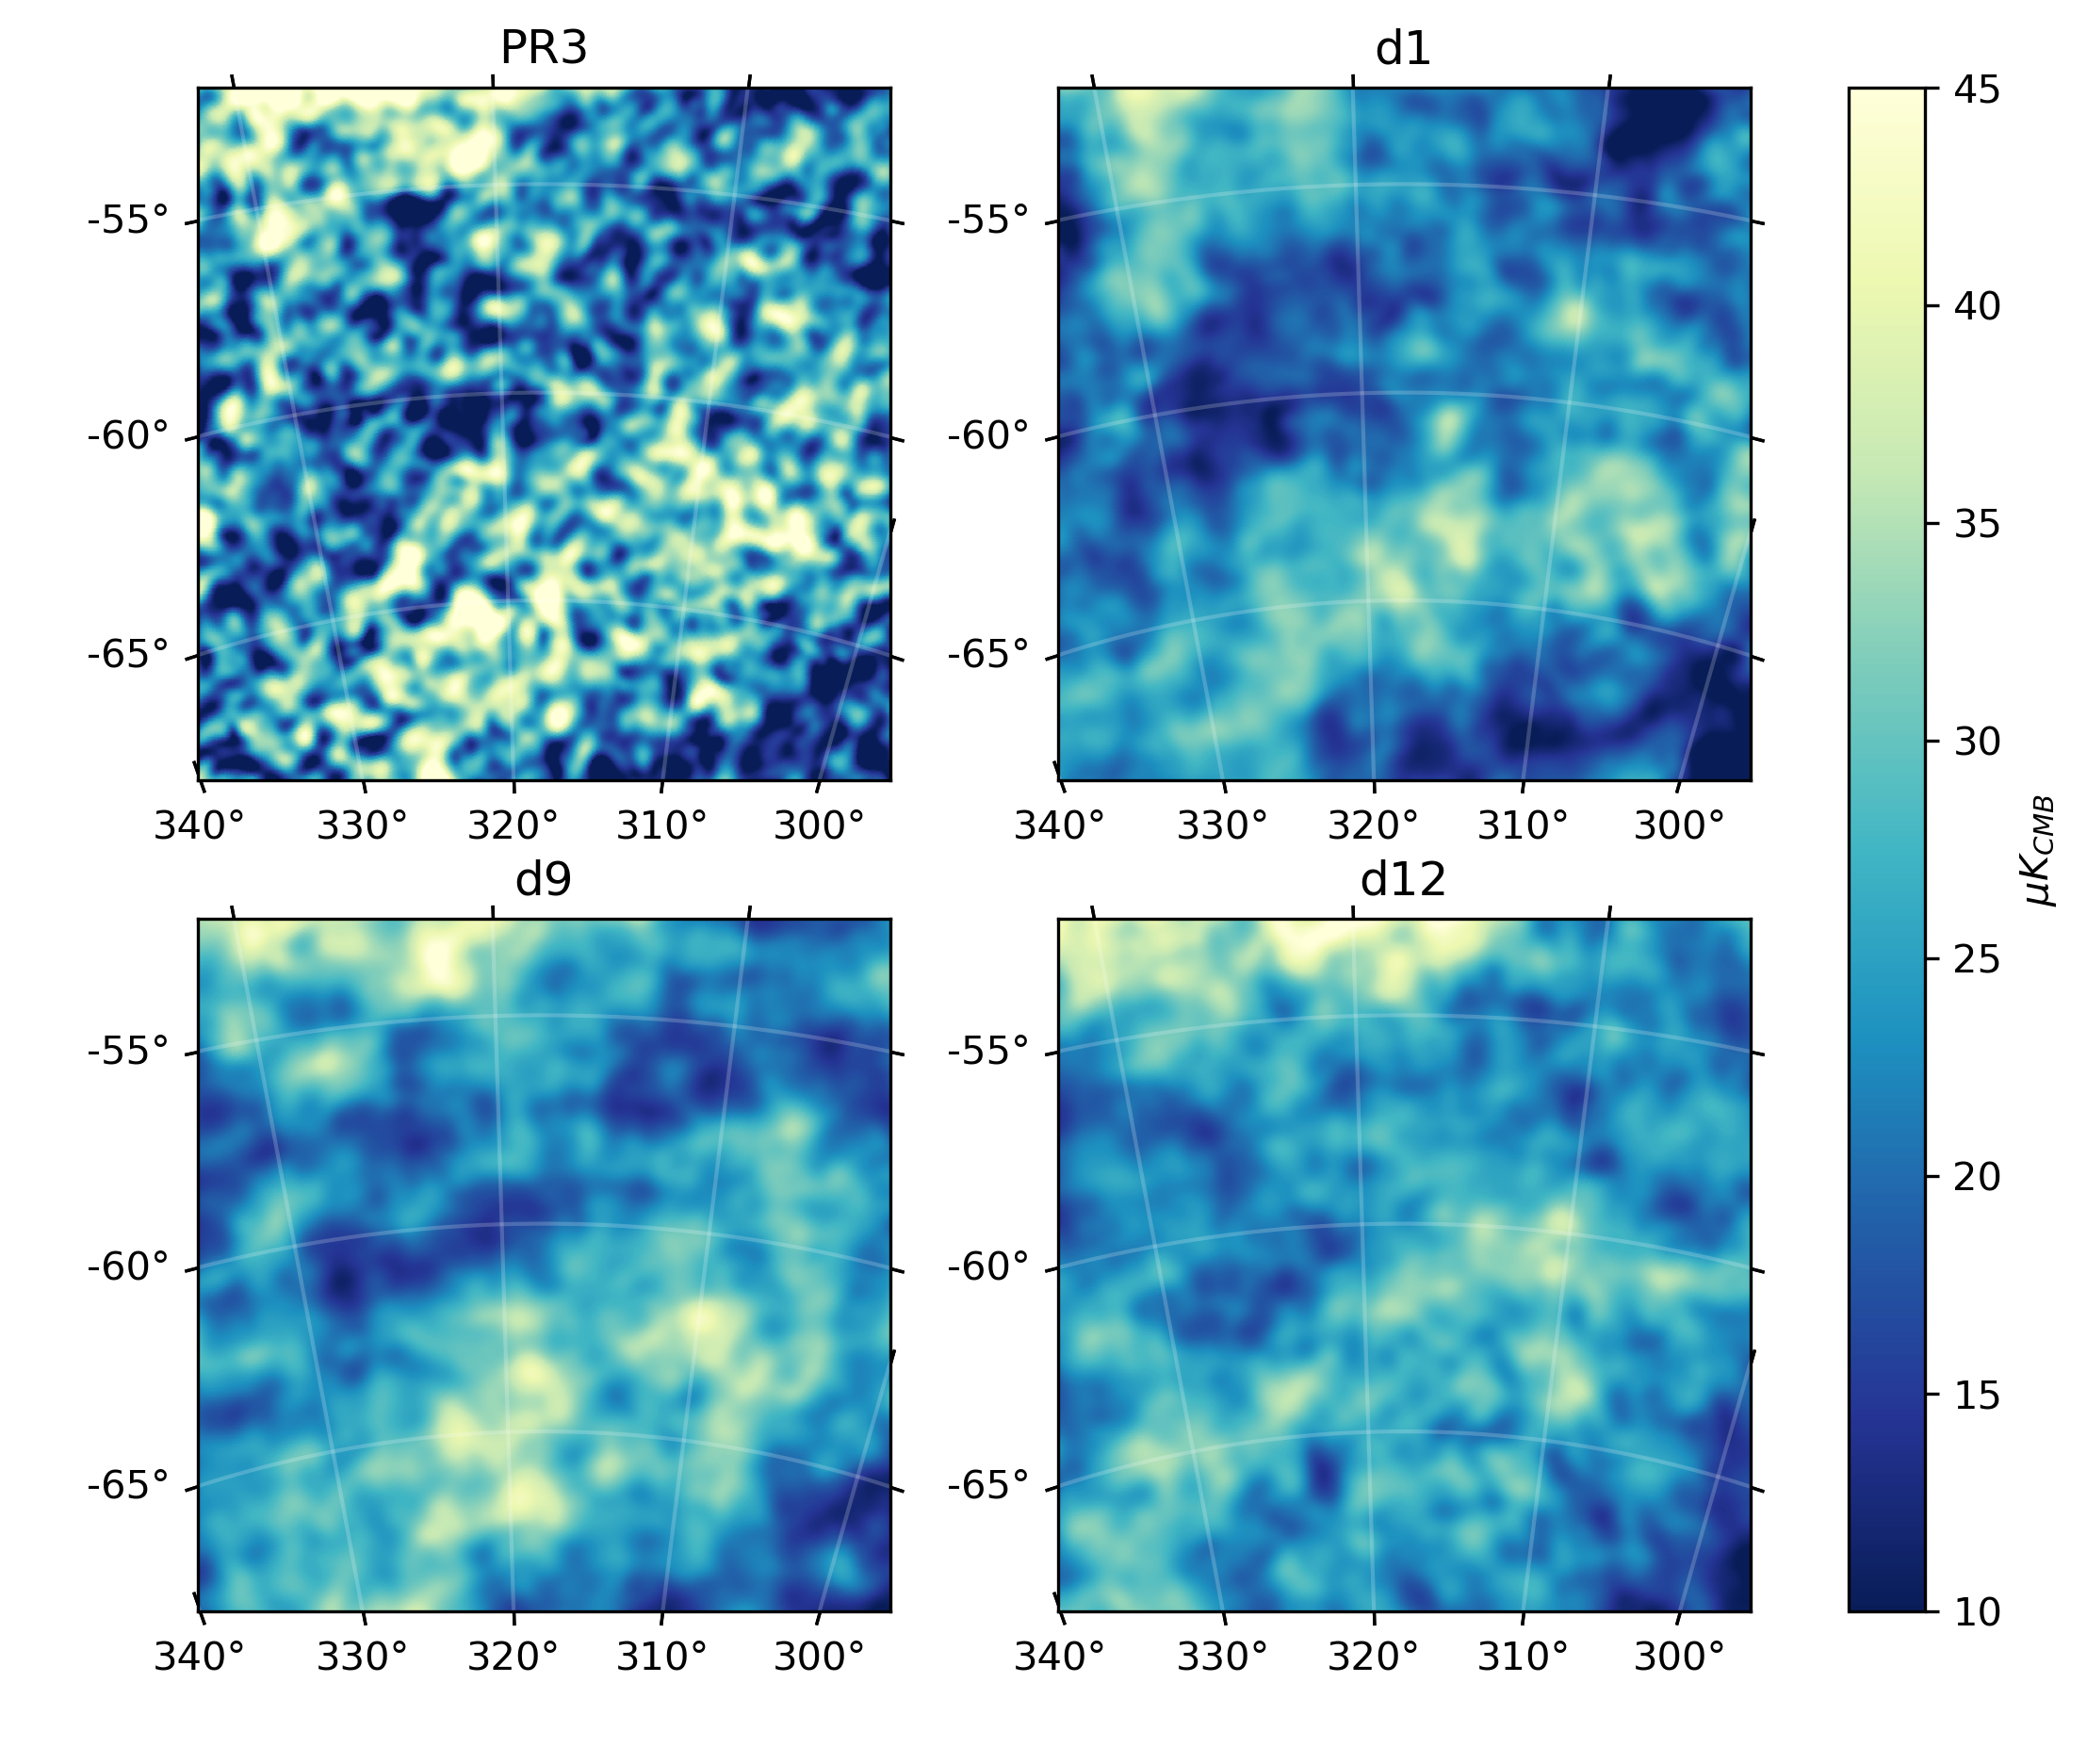
\includegraphics[height=0.41\textwidth]{figures/pol_BK_smooth_30'.png}
    \caption{Polarized dust intensity at 353GHz centered at [l = 180, b = -10] (left) and [l = 318, b = -61] (right), smoothed to $30\arcmin$.}
    \label{fig:353_pol_int}
\end{figure*}

We integrate the dust models in the Planck passband \citep{planck2013-p03d}. For the comparison between total intensity maps, we subtract a Wiener-filtered CMB temperature anisotropy map from SMICA.

Intensity and polarization at 353~GHz are displayed in Figures~\ref{fig:353_int} and \ref{fig:353_pol_int}. 
In intensity, model {\tt d9} filters more of the real data and generates more random small-scale structures than models {\tt d1} and {\tt d12}. We can visually appreciate the impact of this choice in the left panel of Figure~\ref{fig:353_int}, near the Galactic plane. 

Note that the color scale is different for several of the models in the right panel of Fig.~\ref{fig:353_int}. This is because the models have different zero points, mainly due to uncertainty in the CIB monopole. For the generation of model {\tt d12}, a monopole of 0.09~MJy/sr is subtracted from the DR2 GNILC intensity map. In the case of model {\tt d1}, it is due to the difference in the CIB monopole between PR2 and PR3 products, as model {\tt d1} is based on PR2 data.

In Figure~\ref{fig:353_pol_int}, we compare the observations and models for polarized intensity at a resolution of $30\arcmin$, to reduce the effects of instrumental noise in the PR3 data. For both of the regions --- close to the Galactic plane and in the center of the Bicep/Keck patch --- all three models are in reasonable visual agreement with the observations. 

\subsection{Power spectra}
\label{sec:PS-validation}
In this section we discuss the power spectrum validation of the PySM dust and synchrotron models. After introducing the methodology in Section~\ref{subsubsec:methods}, we examine dust and synchrotron emission over large sky areas in Sections~\ref{sec:dust_validation} and \ref{sec:sync_validation}, respectively, and finally analyze the BICEP/Keck patch specifically in Section~\ref{sec:BK_validation}.

\subsubsection{Methodology} \label{subsubsec:methods}
For our large-area validation, we employ sky masks that leave 80\%, 60\%, 40\% and 20\% of the sky unmasked. The mask choices are different for the dust and synchrotron validations due to the varying characteristics of these two emissions. A detailed explanation of the choices is provided in the relevant subsections. 

After masking, we compute the power spectra using the \texttt{anafast} function from healpy\footnote{\url{https://healpy.readthedocs.io}}~\citep{Zonca:2019} and account for the masking effects by dividing the spectra by $f_{\rm sky}$, the second moment of the mask. We do not implement further corrections for mode-mixing caused by masking, as methods for such corrections assume that the field is free from any inherent mode-coupling~\citep[e.g.,][]{Hivon:2002}, which holds for the CMB but not for the highly non-stationary Galactic emission. 

We bin the power spectra into dynamic $\ell$-intervals optimized for map noise and sky fraction. Throughout this work, we present the results as $\mathcal{D}_\ell \equiv \ell(\ell + 1) C_\ell / 2\pi$, where $C_\ell$ is the power spectrum, with all values expressed in $\mu{\rm K^2_{CMB}}$ units. 

Since polarized dust emission is the primary foreground contaminant for CMB $B$-mode observations, we conduct additional validations of dust $B$-mode polarization in small sky patches to examine the properties of the injected small scales. Our results demonstrate that the spatial modulation of the small-scale realizations does not, on average, introduce foreground power excess in high latitude sky regions, an improvement over previous \texttt{PySM} models.

\subsubsection{Dust Emission Over the Sky} 
\label{sec:dust_validation}
To evaluate the performance of the \texttt{PySM} dust models \texttt{d1}, \texttt{d9}, \texttt{d10}, and \texttt{d12} against real data across a wide range of scales, we present their power spectra computed using both large-area and small-area masks at 353~GHz, where the dust emission is dominant. First, we generate \texttt{PySM} dust models maps at a monochromatic frequency of 353~GHz and smooth them with a $4.82\arcmin$ Gaussian beam to match the resolution of the Planck 353~GHz channel. We color-correct the Planck NPIPE 353~GHz channel maps\footnote{\url{https://portal.nersc.gov/project/cmb/planck2020/}}~\citep{PlanckCollaboration:2020} to the same single frequency using a scaling factor 1/1.098~\citep{planck2016-l11A}, and subtract the CMB dipole from the NPIPE temperature maps. We then apply identical masks (defined below) to the mean-subtracted \texttt{PySM} dust models and NPIPE ``A''/``B'' detector-split maps. Finally, we compute the auto-spectra of the model maps and the cross-spectra of the NPIPE data splits using these masks to minimize noise correlation. 

For our large-area comparison, we use a set of $2^\circ$-apodized Galactic masks\footnote{\texttt{HFI\_Mask\_GalPlane-apo2\_2048\_R2.00.fits}} from the Planck Legacy Archive. With eight in total, these masks cover a range of sky fractions, leaving between 20\% and 99\% of the sky unmasked. For our analysis, we take four representative masks: \texttt{GAL020}, \texttt{GAL040}, \texttt{GAL060} and \texttt{GAL080}, where the number in the mask name indicates the percentage of the sky available for analysis, i.e., $100 f_{\rm sky}$.

In Figure~\ref{fig:largefield_power}, we compare the $TT$, $EE$, and $BB$ power spectra of the \texttt{d1}, \texttt{d9} and \texttt{d12} models against the NPIPE map. Since the \texttt{d10} model is identical to the \texttt{d9} model at 353~GHz, it is not shown separately. Error bars on the cross-spectra are derived from 200 NPIPE detector-split simulations.

\begin{figure}
    \centering
    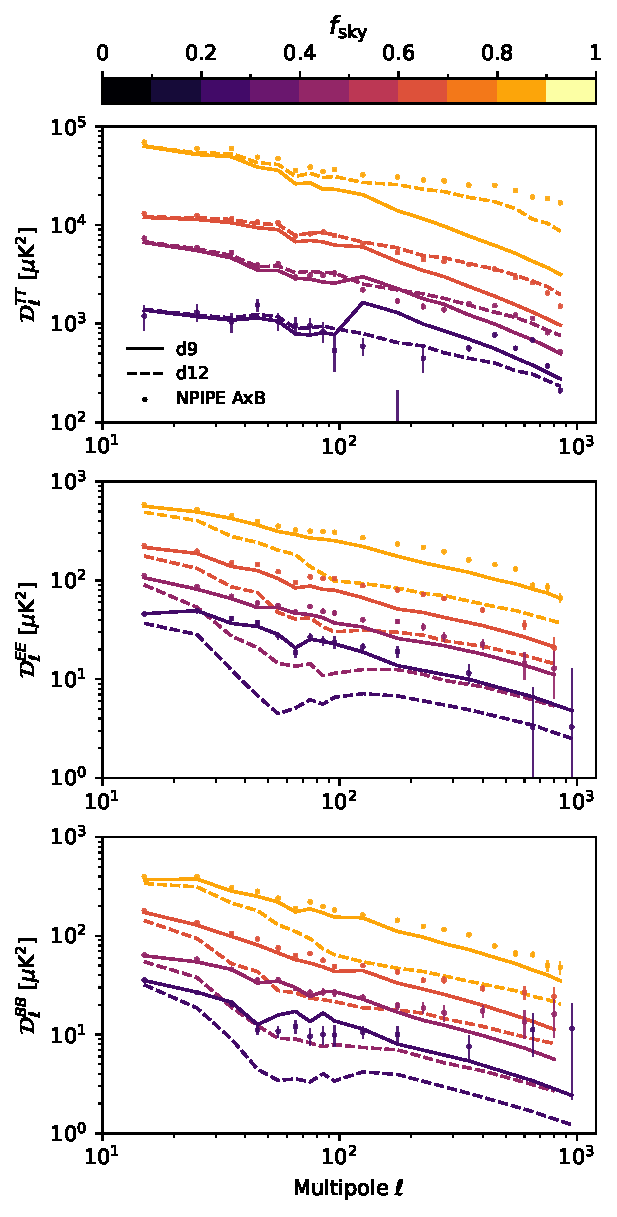
\includegraphics[width=\columnwidth]{figures/largefield_power_all_TEB_pub.pdf}
    \caption{The $TT$, $EE$ and $BB$ power spectra for the \texttt{d1} (dashed lines), \texttt{d9} (solid lines) and \texttt{d12} (dotted lines) models, along with the NPIPE detector-split maps (circles), computed using the \texttt{GAL020}, \texttt{GAL040}, \texttt{GAL060} and \texttt{GAL080} Galactic masks. Each comparison set is colored to represent the respective sky fraction $f_{\mathrm{sky}}$. The \texttt{d10} model is not shown as it is identical to \texttt{d9} at 353~GHz.}
    \label{fig:largefield_power}
\end{figure}

We find that the \texttt{d1} and \texttt{d12} models generally match the observed $TT$ spectrum, although they underestimate the power at $\ell > 500$ when $f_{\rm sky} = 0.8$. The \texttt{d9} model shows similar agreement with observations at $\ell \lesssim 100$ across all sky fractions. However, its power declines more steeply at higher multipoles for $f_{\rm sky} = 0.6$ and $0.8$, and it exhibits a bump in the power spectrum around $\ell \sim 100$ for $f_{\rm sky} = 0.2$ and $0.4$. This artifact occurs because the parameters $l_1$, $c_1$, $c_2$ and $\gamma$ in Equations~\eqref{eq:filter} and~\eqref{eq:filter2}, which control the smoothing of the transition from large-scale template power to small-scale injection power, were optimized for large-sky polarization spectra rather than temperature spectra. 

In polarization, \texttt{d12} significantly underestimates both $EE$ and $BB$ spectra across all scales. On the contrary, both \texttt{d1} and \texttt{d9} align well with $EE$ data across all scales and sky fractions. \texttt{d9} demonstrates generally smooth power transitions for both $EE$ and $BB$ spectra, although some ripple artifacts emerge around $\ell \sim 100$ in smaller $f_{\rm sky}$ cases, again caused by the parameter optimization. The NPIPE $BB$ band power rises at high-$\ell$ presumably due to residual noise dominating smaller sky patches --- a behavior not observed in $\texttt{d9}$, as its small-scale power is derived from template extrapolation. 

\begin{figure}
    \centering
    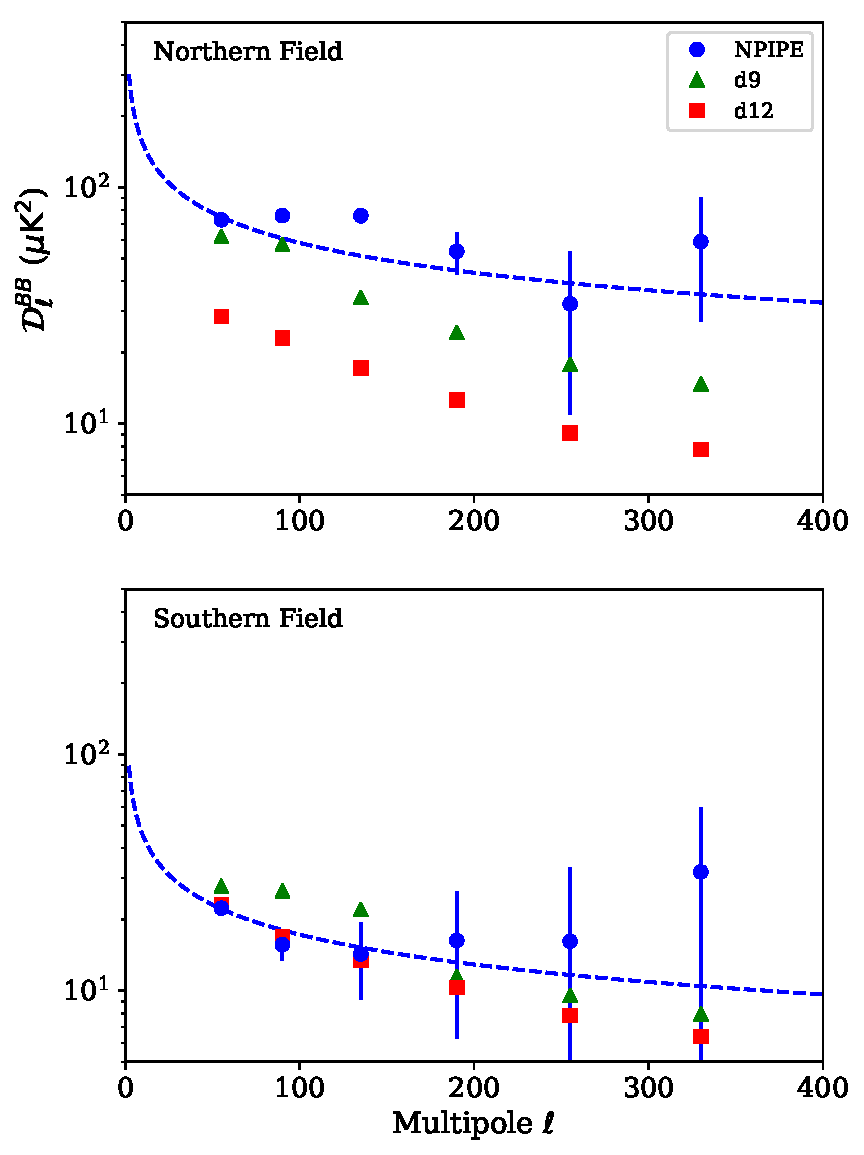
\includegraphics[width=0.48\textwidth]{figures/smallfield_power.pdf}
    \caption{The binned $BB$ power spectra from the 353~GHz NPIPE detector-split maps and the dust model maps \texttt{d1}, \texttt{d9} and \texttt{d12}. The dashed lines indicate the best-fit of the fixed-index power law ($\mathcal{D}_\ell^{BB} = A \, \big( l/80 \big)^{\alpha}$ where $\alpha = -0.54$) to the NPIPE data points, with the fit largely driven by the first two band powers.}
    \label{fig:smallfield_power}
\end{figure}

\begin{figure*}
    \centering
    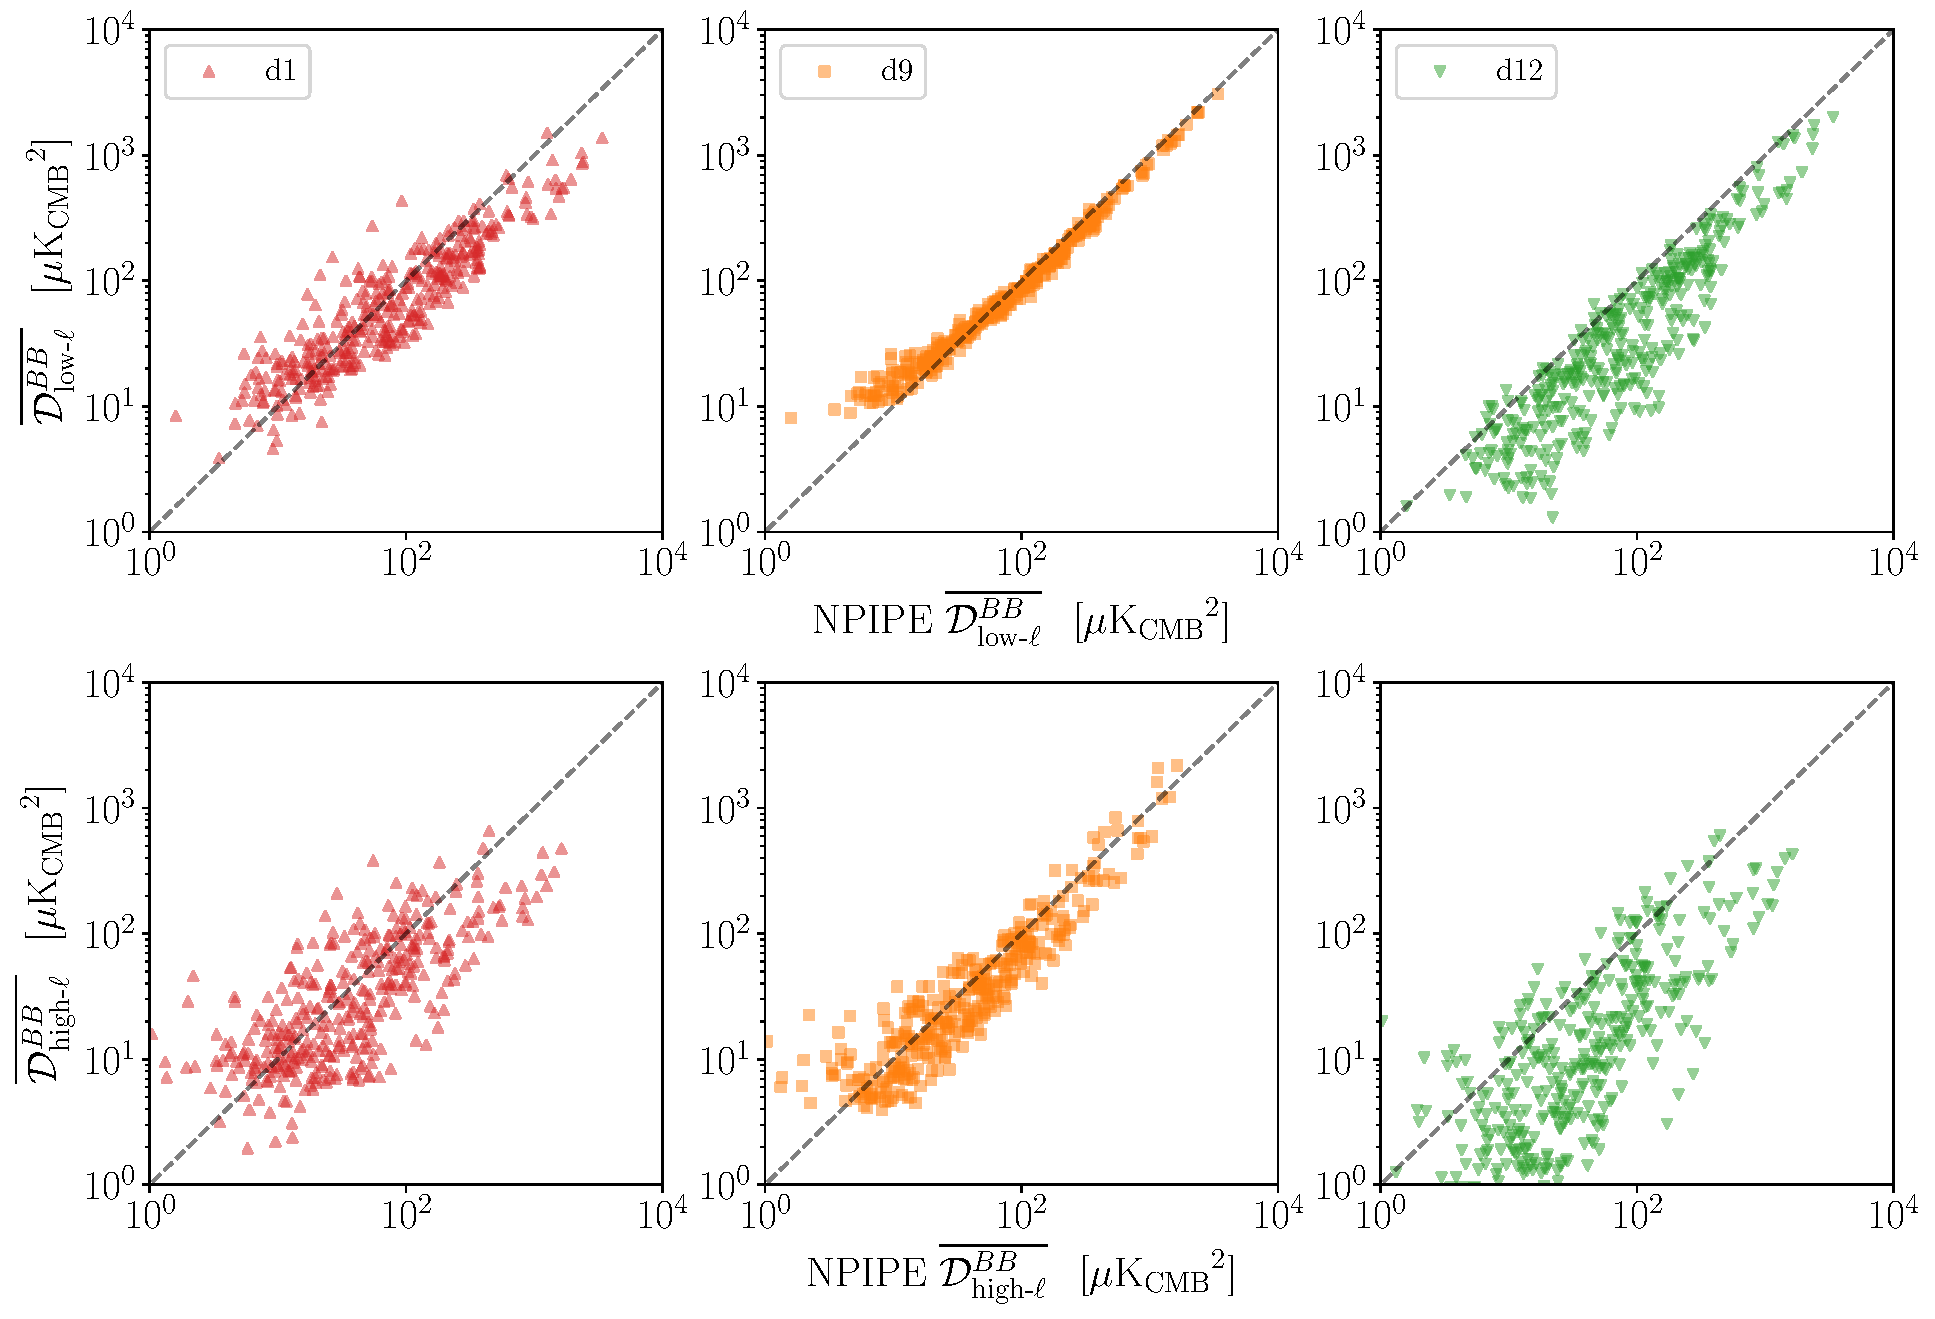
\includegraphics[width=2.1\columnwidth]{figures/llmean_hlmean_comparison.pdf}
    \caption{Scatter plots of the mean of the first two $BB$ band powers, $\overline{\mathcal{D}_{\text{low-}\ell}^{BB}}$, and the mean of the last four $BB$ band powers, $\overline{\mathcal{D}_{\text{high-}\ell}^{BB}}$, as illustrated in Figure~\ref{fig:smallfield_power}. The top panel compares $\overline{\mathcal{D}_{\text{low-}\ell}^{BB}}$ of \texttt{d1}, \texttt{d9}, and \texttt{d12} against that of NPIPE, while the bottom panel shows the same comparison for $\overline{\mathcal{D}_{\text{high-}\ell}^{BB}}$. Each data point represents the results from a circular sky patches with $|b| > 30^\circ$. Dashed lines indicate the 1:1 ratio.}
    \label{fig:smallfield_power_all}
\end{figure*}

For our small-area comparison, we instead follow the method described in \cite{planck2014-XXX} to define the masks for power spectrum computation. The full sky is divided into 768 patches with a HEALPix grid with $N_\text{side} = 8$. At the center of each patch, we construct a circular mask covering 400~deg$^2$, with the edges tapered by a $2^\circ$ FWHM Gaussian, yielding $f_{\rm sky} \sim 0.008$. Figure~\ref{fig:smallfield_power} presents representative results from two selected circular fields located at Galactic latitudes $|b| > 30^\circ$ in the northern and southern Galactic hemispheres. Since the computational cost of running simulations for cross-spectra error calculations in each small patch is high, the errors are estimated using analytical approximations of the cross-correlation matrix of power spectra~\citep{Tristram:2005}.

To assess whether the \texttt{PySM} models can accurately replicate the observed dust $BB$ power spectrum's amplitude and scaling in $\ell$, particularly in small high Galactic latitude fields relevant to future CMB observations, we calculate the low-$\ell$ averaged band power $\overline{\mathcal{D}_{\text{low-}\ell}^{BB}}$ (over $40 \le \ell < 110$) and the high-$\ell$ averaged band power $\overline{\mathcal{D}_{\text{high-}\ell}^{BB}}$ (over $110 \le \ell < 370$) for both the model and NPIPE maps in each small field with $|b| > 30^\circ$. These metrics reduce the impact of noise variation in the NPIPE $BB$ data in the circular sky patches, serving as proxies for comparing dust amplitudes between the model and the data at two different angular scales. The results are presented as scatter plots in Figure~\ref{fig:smallfield_power_all}.

Both the \texttt{d1} and \texttt{d9} models exhibit power amplitudes that are generally consistent with NPIPE, but \texttt{d9} demonstrates a significant improvement in correlation, particularly increasing the correlation coefficient from 0.887 to 0.998 in the low-$\ell$ regime. This improvement stems from the combination of GNILC large-scale templates and small-scale modulation, which is especially evident in regions with a high signal-to-noise ratio, such as in the $\overline{\mathcal{D}_{\text{low-}\ell}^{BB}}$ comparison or in small fields with substantial dust amplitudes. 

However, in fields where $\overline{\mathcal{D}_{\text{low-}\ell}^{BB}}$ and $\overline{\mathcal{D}_{\text{high-}\ell}^{BB}}$ are smaller than 10~$\mu\rm{K^2_{CMB}}$, \texttt{d9} systematically overestimates the dust amplitude. This overestimation is likely due to a positive noise bias present in regions of the GNILC dust maps with low foregrounds, which propagates from large to small scales through the extrapolated power spectrum fit during our model construction. Conversely, $\texttt{d12}$ underestimates the dust amplitude in 94\% (85\%) of the small fields for low-$\ell$ (high-$\ell$). These two separate trends are also observed in individual small fields measured by ongoing $B$-mode experiments, such as the BICEP/Keck field, which will be discussed in Section~\ref{sec:BK_validation}, and in the SPIDER field independently analyzed by \cite{SPIDERCollaboration:2024}, although the latter results are presented at 150~GHz. 

For the comparison of scaling in $\ell$, we introduce the ratio $\mathcal{R} \equiv \overline{\mathcal{D}_{\text{low-}\ell}^{BB}} \Big/ \overline{\mathcal{D}_{\text{high-}\ell}^{BB}}$ as another metric to describe changes in spatial power across the modulation scale. According to this definition, the fixed-index power law $\mathcal{D}_\ell^{BB} \propto \ell^{-0.54}$, derived from the analysis of a larger sky region with $f_\text{sky} = 0.8$ by \cite{planck2016-l11A}, yields a value of $\mathcal{R} = 1.83$. This estimate is closely aligned with the small-field NPIPE data, which give a value of $\mathcal{R} = 1.85 \pm 0.93$. The \texttt{d1}, \texttt{d9}, and \texttt{d12} models instead produce slightly higher values: $\mathcal{R} = 2.03 \pm 0.72$, $\mathcal{R} = 2.35 \pm 0.77$ and $\mathcal{R} = 2.26 \pm 0.91$ respectively. While the injected small scales in \texttt{d9} are also generated using an index of $\alpha = -0.54$ (Table~\ref{tab:smallscale_par}), this fit is performed in the $bb$ spectrum. 

During the development of the \texttt{PySM} models presented in the present study, we used the ratio $\mathcal{R}$ as a key proxy to track the transition of band power from large scales to small scales in small-area cases. This approach ultimately guided us to adopt the improved modulation map construction method discussed in Section~\ref{subsec:methodology}, ensuring a smooth transition between scales. The remaining discrepancy in \texttt{d9} can be attributed to the non-linear transformation between $D_\ell^{bb}$ and $D_\ell^{BB}$.

\subsubsection{Synchrotron Emission Over the Sky} \label{sec:sync_validation}

In this section, we detail the validation of the new synchrotron models by comparing the power spectra with observations. For validating the \texttt{PySM} synchrotron temperature models, we use the synchrotron map\footnote{\url{https://beyondplanck.science/products/files\_v1}} from the BeyondPlanck re-analysis of Planck LFI data \citep{Andersen:2023}. This map is at a reference frequency of 30\,GHz and has an angular resolution of $2^\circ$. We produce single-frequency temperature maps for the different synchrotron models at 30\,GHz and smooth with a Gaussian beam with FWHM = $2^\circ$.

We have purposely chosen an earlier release of BeyondPlanck for our analysis. Later data release versions of BeyondPlanck, or its successor CosmoGlobe, produce synchrotron intensity maps at 408~MHz~\citep{Watts:2023}. The PySM synchrotron models \texttt{s5} and \texttt{s7} are not suitable for producing synchrotron simulations at 408\,MHz. This is a consequence of scaling the Haslam map from 408\,MHz to 30\,GHz with a constant $\beta_s$ for constructing the template for synchrotron intensity and then applying a spatially variable $\beta_s$ to evaluate the model (see Section~\ref{subsec:spec_params_overview}). Therefore, we validate our models with the synchrotron intensity map at 30\,GHz.

For synchrotron polarization validation, we compare the models with Planck Revisited synchrotron polarization maps\footnote{\url{https://portal.nersc.gov/project/cmb/Planck\_Revisited}} \citep{Delabrouille:2024}. These are the lowest-noise full sky maps of polarized synchrotron at 30\,GHz at $1^\circ$ resolution at the time of analysis. 

\begin{figure}
    \centering
    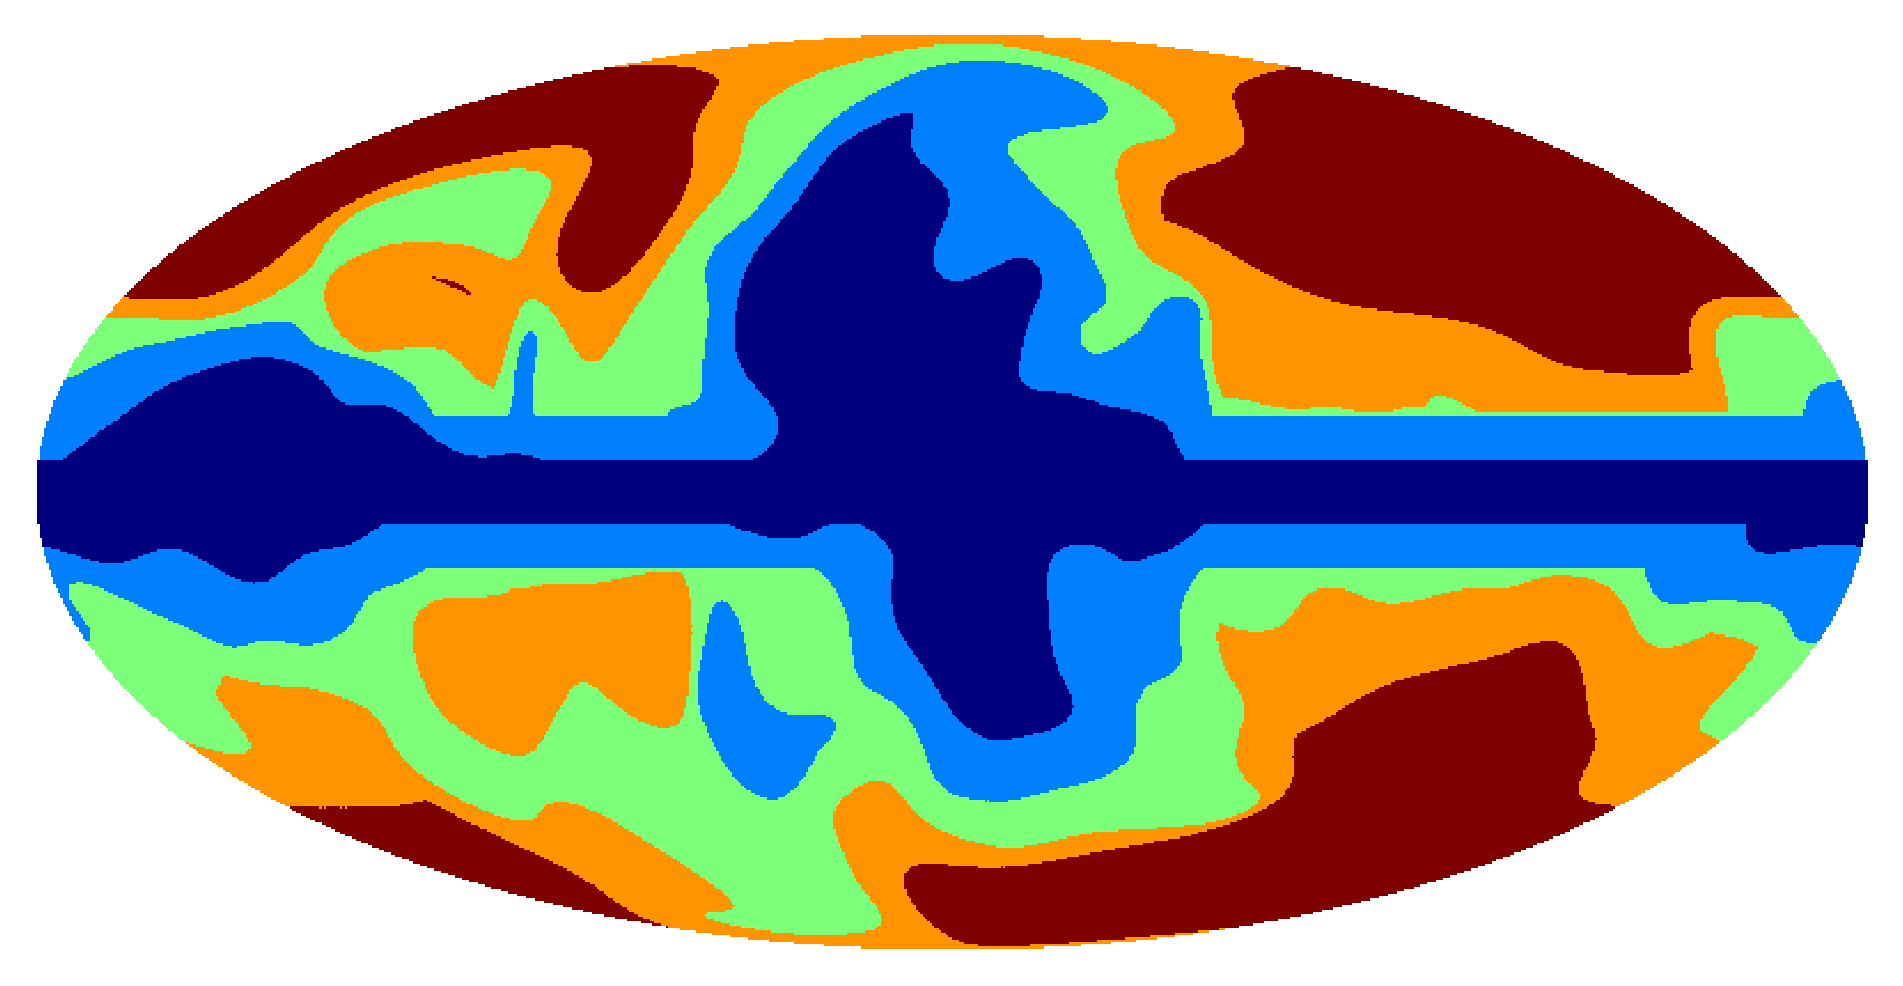
\includegraphics[width=0.46\textwidth]{figures/SYNC_mask_stack.png}
    \caption{The four different Galactic masks used for the synchrotron validation. The red region is the 20 \% mask; the orange region shows the additional sky coverage for 40 \% mask; the yellow region shows the added coverage for 60 \%; the green region is the added sky patch of 80 \% mask. The purple region is excluded in all masks.}
    \label{fig:sync_masks}
\end{figure}

We do not use the Planck Galactic masks for the synchrotron power spectra validation. The Planck Galactic masks capture the shape of the Galactic dust signal, as it is the brightest foreground at CMB frequencies. The shape of the Galactic synchrotron signal differs significantly from the shape of the Galactic masks. Therefore, we construct masks for the synchrotron by thresholding the synchrotron polarized intensity smoothed with a $8.5^\circ$ beam. We additionally mask out a portion of the Galactic plane with a narrow band mask. This ensures that we are always excluding the Galactic plane. In Figure~\ref{fig:sync_masks} we show the coverages of these masks. 

\begin{figure}
   \centering
   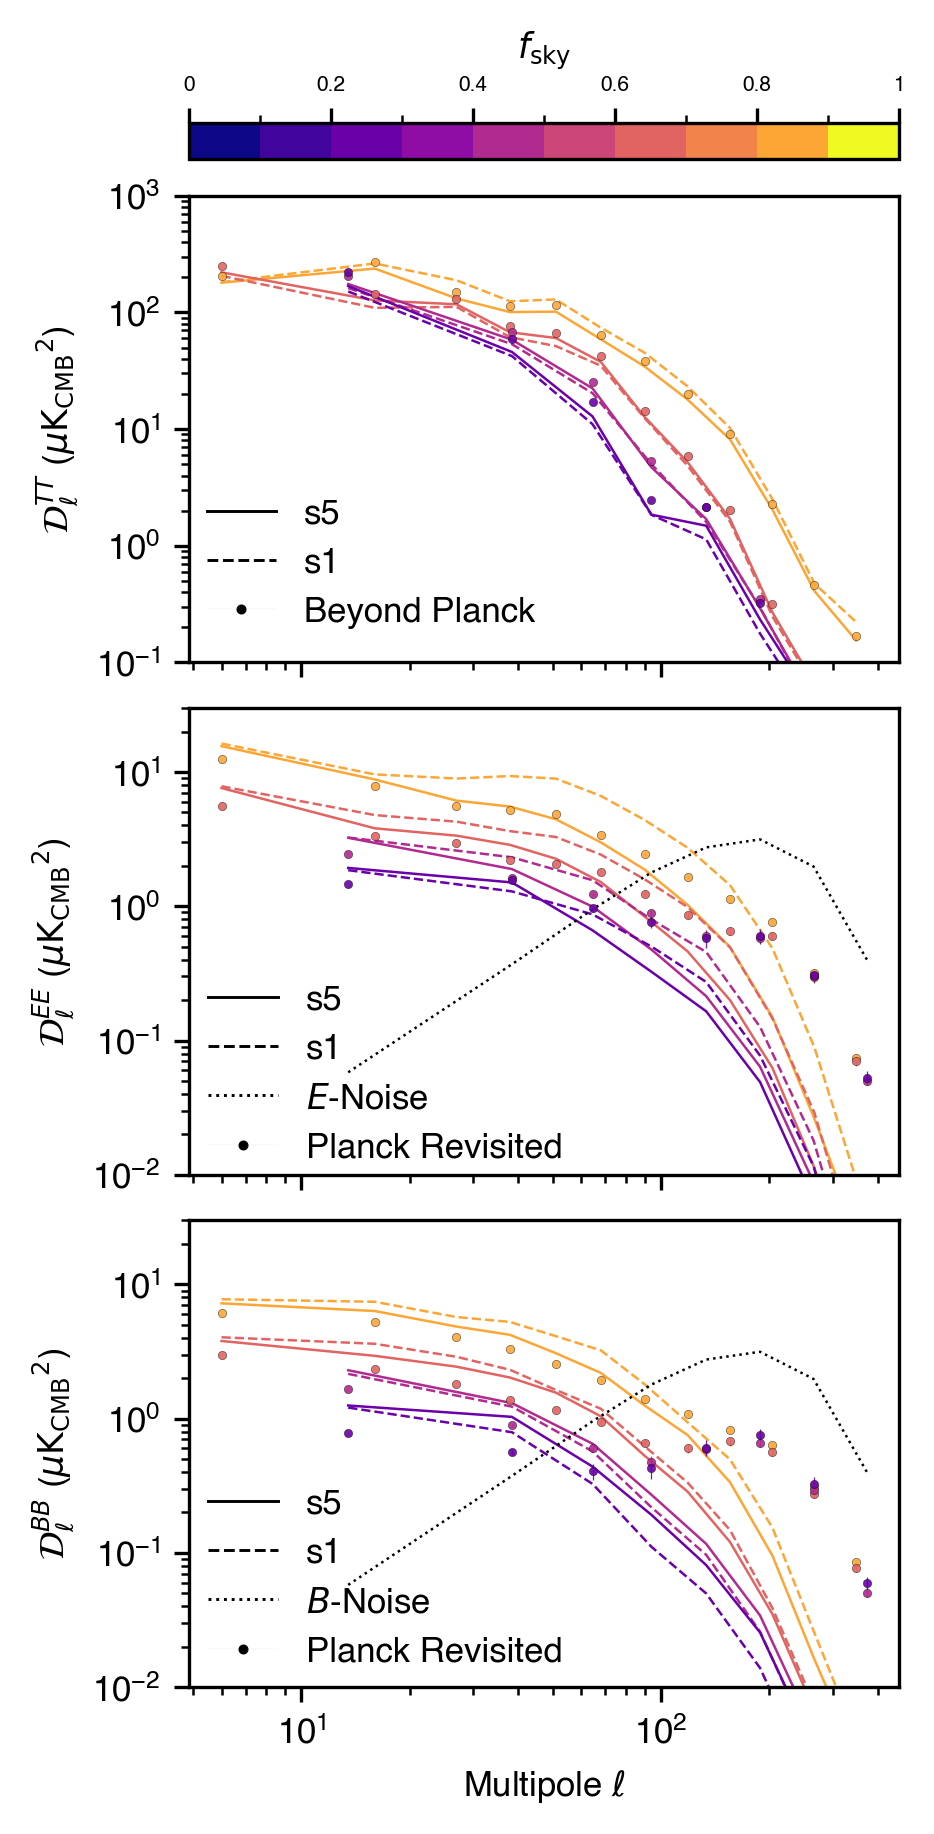
\includegraphics[width=0.48\textwidth]{figures/Dlcomp_PySM3-4_s5_vs_BPPR_SYNC.png}
    \caption{Comparison of the \texttt{PySM} \texttt{s1} and \texttt{s5} power spectra with observations over different sky fractions. The observed $TT$ power spectra are computed from the synchrotron intensity map from  BeyondPlanck Release 1~\citep{Andersen:2023} at 30~GHz with a $2^\circ$ beam. The observed $EE$ and $BB$ power spectra are derived from the Planck Revisited~\citep{Delabrouille:2024} polarized synchrotron map at 30~GHz with a $1^\circ$ beam. These $EE$ and $BB$ spectra are debiased for noise, calculated from 200 simulations, and the noise power spectra are also displayed to highlight the change of signal-to-noise ratio across the multipole range.}
   \label{fig:Dl_sync_galmask}
\end{figure}

For the polarization analysis, we further apply the Planck Revisited point source mask to exclude the brightest point sources. The combined mask is apodized with a $2^\circ$--$6^\circ$ cosine taper, with the apodization length increasing as the sky fraction decreases. Using 200 noise realizations, we compute the mean and standard deviation of the noise spectra. The polarization power spectra are then noise-debiased, with error bars reflecting the noise standard deviation.

In Figure~\ref{fig:Dl_sync_galmask} we present $TT$, $EE$ and $BB$ power spectra comparisons for models \texttt{s1} and \texttt{s5}. Since models \texttt{s4}, \texttt{s6} and \texttt{s7} yield nearly identical results, we display only the results for model \texttt{s5}. The $TT$ power spectra across all sky fractions for both models show excellent agreement with the BeyondPlanck synchrotron temperature power spectra. For the $EE$ power spectra, model \texttt{s5} demonstrates good agreement in the multipole range where signal-to-noise is $\gtrsim 1$ for the Planck Revisited polarized synchrotron power spectra. In contrast, model \texttt{s1} exhibits higher power for most multipoles compared to the Planck Revisited $EE$-synchrotron spectrum for the 80\% and 60\% sky fractions, although they align well for the 40\% and 20\% sky fractions. We also observe a distinct change in the shape of the $EE$ power spectrum for the \texttt{s1} model around the injection scale, $\ell_*\sim 36$ \citep{Thorne:2017}. The improved performance for model \texttt{s5} comes from the empirical optimization of the filters in Equation~\eqref{eq:filter}. Both models have higher $BB$ power for 80\% and 60\% sky fractions, but model \texttt{s1} shows better agreement with observations for smaller sky fractions.

For $\ell \sim 200$, we find a bump in spectrum for the Planck Revisited observations. This is likely caused by our inability to perform noise debiasing where the signal-to-noise ratio is low. However, the combined effect of residual point sources and incorrect masking choices may also contribute to the residual bias. Based on the current results, we conclude that while our synchrotron models are validated for $\ell \lesssim 300$ for intensity, they are only consistent with observations up to $\ell \lesssim 100$ in polarization due to limited signal-to-noise of the polarized synchrotron data at smaller scales.

\subsubsection{Dust and Synchrotron Emission in the BICEP/Keck Patch}
\label{sec:BK_validation}
\begin{figure*}
    \centering
    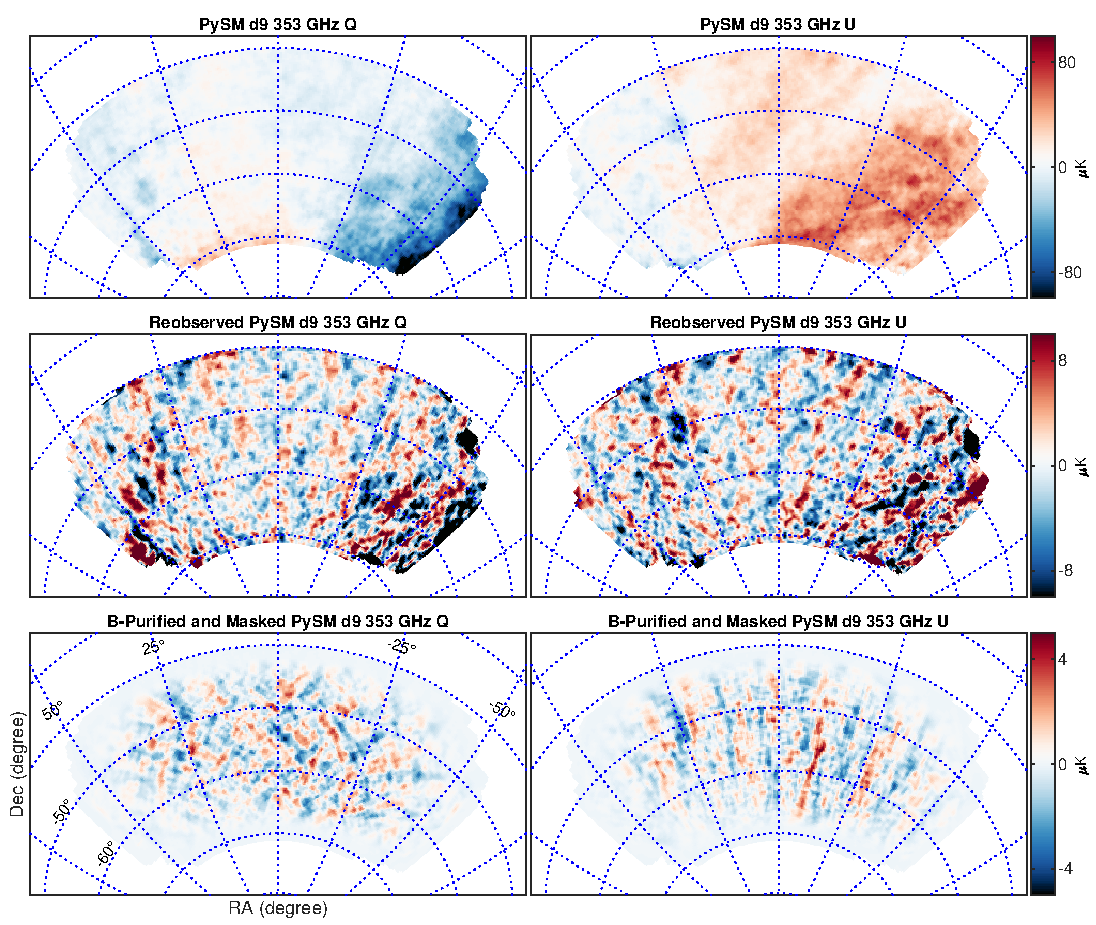
\includegraphics[width=2.\columnwidth]{figures/pysm_d9_353_delta_reobs_B_pub.pdf}
    \caption{The \texttt{PySM} \texttt{d9} maps, reobserved maps and purified maps in the BICEP/Keck sky patch at 353\,GHz. Each panel shows the
    \texttt{PySM} $Q$ and $U$ maps reprocessed by the BK18 BICEP3 beam profile, observation matrix, and purification matrix respectively.}
    \label{fig:psym_BKmatrix}
\end{figure*}

The cleanest patch of sky in the southern hemisphere is particularly crucial for ongoing and future CMB experiments aimed at measuring primordial $B$-mode polarization. The most powerful data set for constraining the tensor-to-scalar ratio $r$ to date comes from the BICEP/Keck (BK) experiment~\citep[``BK18'';][]{Ade:2021}. This data set includes BK observations up to the 2018 observation season, covering a $\sim 600$ square degree sky patch centering at RA 0h, Dec. $-57.5^{\circ}$, and incorporates the NPIPE and WMAP across the 23--353~GHz range from the same region. In the coming years, a collaborative effort between the BICEP/Keck and the South Pole Telescope (SPT) will combine the BICEP3 and BICEP Array maps with overlapping SPT-3G maps to ``delens'' the observed CMB $B$-modes, further tightening constraints on $r$~\citep{TheBICEP/KeckCollaboration:2024}. Given that this observation field will also overlap with the planned survey area for the CMB-S4 experiment's primordial $B$-mode search \citep{Abazajian:2022}, there will be sustained interest in simulating Galactic foregrounds in this region, justifying a dedicated analysis. 

\begin{figure}
    \centering
    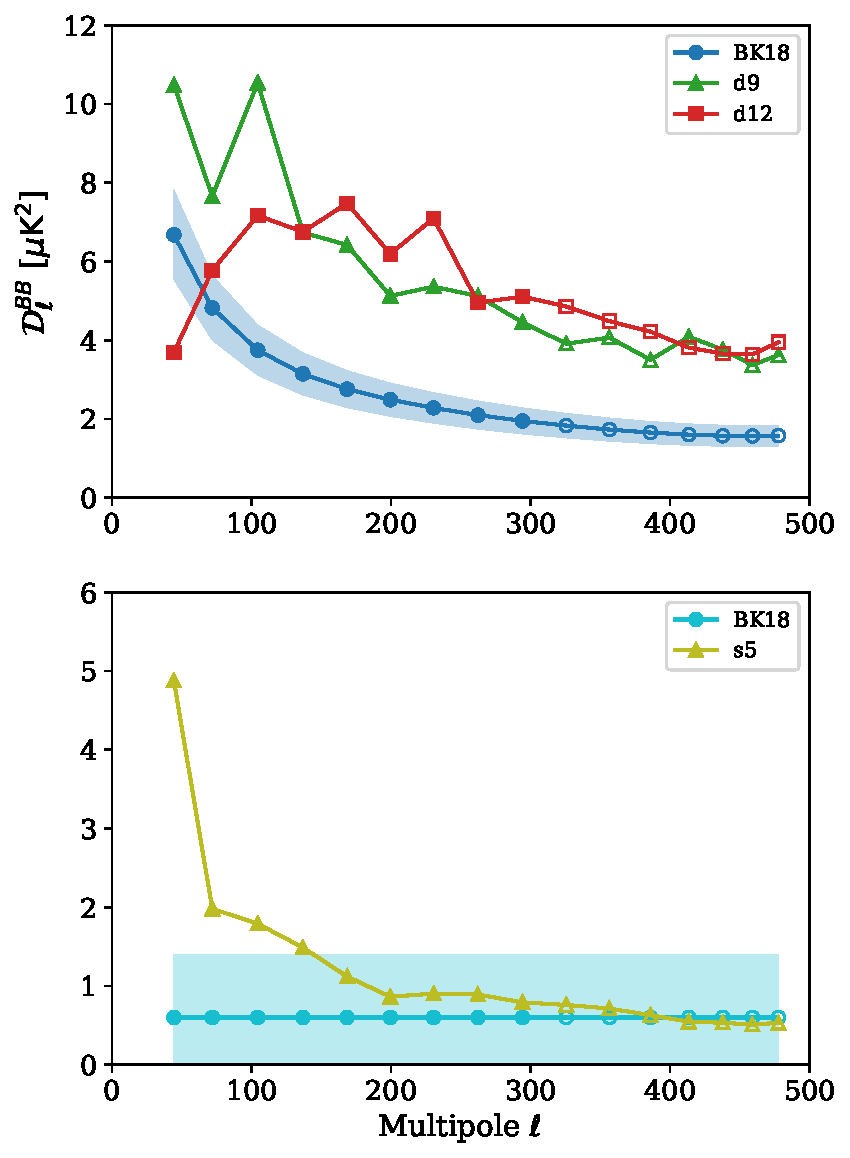
\includegraphics[width=0.48\textwidth]{figures/BKfield_power.pdf}
    \caption{Comparison of the \texttt{PySM} and NPIPE $BB$ power spectra for the BK patch with the BK18 maximum likelihood models. The top panel shows the results of dust at 353~GHz, while the bottom panel presents the synchrotron results at 23~GHz. These nine band powers correspond to the BK science bins used for delivering constraints. The shaded area and the arrow symbol represent the uncertainties in foreground amplitudes: $\pm 0.75 \; \mu\rm{K^2_{CMB}}$ for dust and a 95\% upper limit of $1.4 \; \mu\rm{K^2_{CMB}}$ at $\ell = 80$ for synchrotron, as derived from BK18 MCMC constraints.}
    \label{fig:BKfield_power}
\end{figure}

To address this need, we utilize the analysis method illustrated in Figure~\ref{fig:psym_BKmatrix}, which shows \texttt{PySM} dust model \texttt{d9} maps that have been ``reobserved'' to replicate the impact of the BK timestream processing and map-making pipeline. In the first panel, the \texttt{d9} $Q$ and $U$ maps at 353~GHz (delta function bandpass) are masked to the BICEP3 observation region and convolved with the BICEP3 beam. The second panel displays the results after these smoothed maps are multiplied by the BK18 BICEP3 observation matrix, simulating the data reduction steps, such as filtering applied along RA scans and beam deprojection in the linear map-making process~\cite{BICEP2Collaboration:2016}. This process results in output maps that appear as if they have been observed and analyzed through the BICEP3 pipeline, where large-scale structures are filtered out, and the amplitude of fluctuations is reduced by a factor of ten. In the third panel, the intermediate maps are multiplied by the corresponding purification matrix to remove $E$-$B$ mixing, producing pure $B$-mode dominated $Q$ and $U$ maps with distinct ``cross-like'' and ``plus-like'' pattern respectively. Finally, the inverse noise-variance apodization mask is applied to yield the science maps. 

By applying the same process to other \texttt{PySM} models at frequencies of interest (\texttt{s1}, \texttt{s4}, \texttt{s5}, \texttt{s6}, \texttt{s7} at 20, 23, 30, 40~GHz and \texttt{d1}, \texttt{d9}, \texttt{d10}, \texttt{d12} at 85, 150, 220, 270, 353~GHz), we generate a set of BK pipeline-propagated, pure $B$-mode model foreground maps that are comparable with BK measurements. We then calculate their $BB$ auto power spectra using the BK binning and present selected results. The color-corrected and noise-biased NPIPE $BB$ power spectrum at 353~GHz, derived from the NPIPE real and simulation maps processed using the same BK analysis method\footnote{\url{http://bicepkeck.org/bk18_2021_release.html}}, are also shown in this section. 

In Figure~\ref{fig:BKfield_power}, we show the $BB$ band power at 353~GHz for the \texttt{d1}, \texttt{d9}, and \texttt{d12} models, along with the band power at 23~GHz for the \texttt{s1} and \texttt{s5} models---these are the reference frequencies adopted in the BK analyses as well as the PySM models. These PySM power spectra are compared to the NPIPE power spectrum and the BK18 maximum likelihood foreground model, which consists of a modified blackbody power spectrum (with $T_d$ fixed at $19.6~\text{K}$) for dust, characterized by parameters $A_{d,\ell=80} = 4.4 \; \mu\rm{K^2_{CMB}}$, $\beta_d = 1.5$ and $\alpha_d = -0.66$, and a power-law synchrotron spectrum with parameter $A_{s,\ell=80} = 0.6 \; \mu\rm{K^2_{CMB}}$, $\beta_s = -3.0$ and $\alpha_s = 0.00$. The BK18 model lines are further suppressed by their band power window functions to account for the mode loss and coupling induced by the matrices. All band powers are eventually converted to full-sky $D_\ell$ by dividing by the integral of the band power window function.

All models exhibit excess dust $BB$ power relative to the measured values in this sky patch at 353~GHz. Among them, \texttt{d1} overestimates the amplitude by about a factor of three---the largest discrepancy---and its small-scale spectrum does not follow a power law, leading to values approximately twice as high as the other models. In contrast, \texttt{d9} and \texttt{d12} power show smaller deviation ratios and generally reproduce the spatial variations observed in the BK data, although \texttt{d12} shows a drop in power at low-$\ell$. This decline is attributed to its suppressed large-scale polarization intensity within the RA range of $[25^{\circ}, 50^{\circ}]$, contrasting with the continuous fluctuations illustrated in Figure~\ref{fig:psym_BKmatrix}.

At large angular scales $\ell \lesssim 100$, the new \texttt{PySM} models are largely influenced by their underlying GNILC templates, while the BK18 constraints on dust $BB$ power come primarily from BK measurements at 220~GHz. The NPIPE power spectrum in the same plot reveals that the variations seen in the first three band powers of the \texttt{d9} model are directly inherited from its large-scale templates. The remaining amplitude discrepancy is likely caused by a noise bias present in the GNILC maps.

Table~\ref{tab:BB_dustratio} further explores how the model amplitudes vary across frequencies, presenting the deviation ratios down to 85~GHz. \texttt{d9} consistently maintains a deviation factor of around two, while \texttt{d1} and \texttt{d10} deviate less from the measurecalcacaments at lower frequencies. This suggests that these models have too large a value of $\beta_d$ relative to the BK model value of 1.5 in this patch. The frequency-dependent trend observed in \texttt{d12} is incompatible with a simple change of $\beta_d$ and likely reflects the multiple-layer behavior inherent to this model. 

\begin{deluxetable}{lccccc}
    \caption{Comparison to BK18}
     \tablehead{& \colhead{85~GHz} & \colhead{150~GHz} & \colhead{220~GHz} & \colhead{270~GHz} & \colhead{353~GHz}}
    \startdata
    \texttt{d1}  & 2.42	& 2.63 & 2.81 & 2.94 & 3.13 \\
    \texttt{d9}  & 2.17 & 2.12 & 2.08 & 2.06 & 2.03 \\
    \texttt{d10} & 0.96 & 1.30 & 1.59 & 1.77 & 2.03 \\
    \texttt{d12} & 2.76	& 2.27 & 2.08 & 2.02 & 1.96 \\
    \enddata
    \tablecomments{The deviation ratio of the reobserved \texttt{PySM} dust $BB$ spectrum to the BK18 maximum likelihood model at each frequency. These ratios are derived by fitting the BK18 model to the \texttt{PySM} band power at their science bins.}
    \label{tab:BB_dustratio}
\end{deluxetable}

Overall, the \texttt{d9} and \texttt{d10} models demonstrate substantial improvements over \texttt{d1}, particularly in their ability to extrapolate the large-scale templates and capture the preferred small-scale power decay that the NPIPE data are unable to reveal in this specific field. However, while the discrepancies in amplitude are reduced, they still persist when compared to the BK18 measurements. Since the aim of this work is not to provide full sky simulations that perfectly align with all available full-sky and partial-sky observations, completely resolving these differences lies beyond its scope. Current power spectrum-based modeling techniques require a certain degree of global averaging of spectrum parameters, which are known to vary across the sky in small patches~\citep{planck2016-l04}. For instance, while dust amplitude can be modulated using large-scale templates, the spectral tilt $\alpha_d$ has to be fixed to a single value for the entire sky, which is inherently unrealistic. Further refinement of new models will be left for future studies. 

Lastly, we compare the synchrotron models with the BK results, focusing on \texttt{s1} and \texttt{s5}, as other new models yield similar outcomes. As illustrated in the lower panel of Figure~\ref{fig:BKfield_power}, both \texttt{s1} and \texttt{s5} display excess power at $\ell \lesssim 100$ and a clear non-zero $\alpha_s$ at 23~GHz. However, this trend reverses at 40~GHz, where the large-scale power of the BK18 maximum likelihood line exceeds that of \texttt{s1} and \texttt{s5} by several times, suggesting that these models have $\beta_s$ smaller than -3. The power spectrum discrepancies at low-$\ell$ between models and data are likely because the models rely on the WMAP 23~GHz map as a template only up to $\ell = 38$, whereas the NPIPE 30/40~GHz maps, which favor a smaller $A_s$, also contribute to the BK constraints~\citep[][Figure~21]{Ade:2021}. Unlike $A_s$, it is important to note that the current BK data impose weak constraints on the parameters $\alpha_s$ and $\beta_s$. These discrepancies will be worth revisiting when new measurements from the BICEP Array telescope, especially its dedicated 30/40~GHz receiver, become available~\citep{Moncelsi:2020}.

\subsection{Decorrelation} \label{subsec:decorrelation}

One of the most challenging aspects of dust emission for CMB analyses is that its frequency dependence varies across the sky. If dust had the same SED everywhere, it would be sufficient to measure it at a frequency where it dominates the submillimeter emission and then subtract off all emission in lower frequency maps that is correlated with that template. The extent to which a map of dust emission at one frequency differs from a map of dust emission at a different frequency (aside from an overall normalization) is referred to as ``frequency decorrelation''. Frequency decorrelation has been identified as a major uncertainty for ongoing and upcoming analyses \citep{Ade:2021}.

The level of decorrelation between two frequencies $\nu_1$ and $\nu_2$ can be quantified by the spectral correlation parameter $R_\ell$, defined as

\begin{equation} \label{eq:R_ell}
    \mathcal{R}^{XY}_\ell(\nu_1\times\nu_2) = \frac{\mathcal{D}_\ell^{XY}(\nu_1\times\nu_2)}{\sqrt{\mathcal{D}_\ell^{XY}(\nu_1\times\nu_1)\mathcal{D}_\ell^{XY}(\nu_2\times\nu_2)}}
    ~~~,
\end{equation}
where $X$ and $Y$ can be any of $T$, $E$, or $B$ \citep{planck2016-L}. Here we focus on $R_\ell^{BB}$.

The 353 and 217\,GHz Planck channels have the highest sensitivity to polarized dust emission and so furnish the current best constraints on the level of dust decorrelation. Analyzing 71\% of the sky over multipoles $50 \leq \ell \leq 160$, \citet{planck2016-l11A} found $R_\ell^{BB} > 0.991$ (97.5\% confidence) between these two frequencies.

\begin{figure}
    \centering
    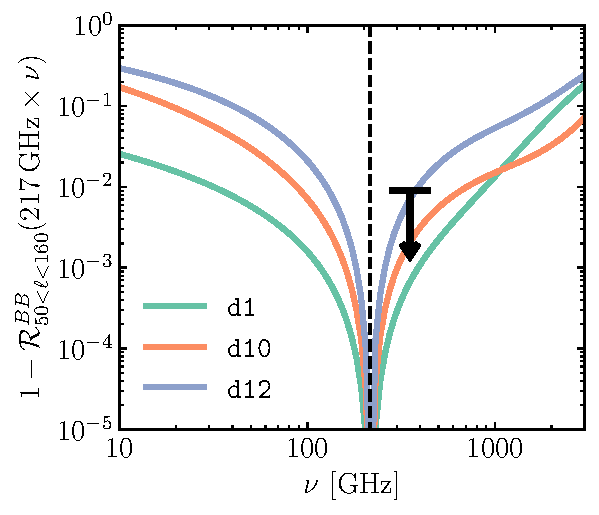
\includegraphics[width=\columnwidth]{figures/decorrelation_dust.pdf}
    \caption{The decorrelation parameter $1-R_\ell^{BB}$, where $R_\ell^{BB}$ is the correlation parameter defined in Equation~\eqref{eq:R_ell}, for the \texttt{d1}, \texttt{d10}, and \texttt{d12} dust models between a reference frequency of 217\,GHz and variable $\nu$. $R_\ell^{BB}$ is evaluated between $50 \leq \ell \leq 160$ over the Planck 70\% sky mask. The 95\% upper limit on decorrelation derived by \citet{planck2016-l11A} over 71\% of the sky is indicated by the black arrow at 353\,GHz. The models span a large range in decorrelation level and each has a distinctive dependence on frequency.}
    \label{fig:decorrelation}
\end{figure}

In Figure~\ref{fig:decorrelation}, we compare the \texttt{d1}, \texttt{d10}, and \texttt{d12} models to this upper limit and analyze more generally how the level of decorrelation with respect to the 217\,GHz map changes with frequency. For each model, we compute $R_\ell^{BB}\left(217\times\nu\right)$ over the multipole range $50 \leq \ell \leq 160$ over the Planck \texttt{GAL070} mask as a function of $\nu$. We adopt a uniform weighting to average the spectra over the broad multipole bin since $\mathcal{D}_\ell^{BB}$ for dust scales roughly as $\ell^{-0.5}$ (see Table~\ref{tab:smallscale_par}). However, nearly identical results are obtained with uniform weighting in $C_\ell$ instead.

We find that all three models respect the upper limit set by \citet{planck2016-l11A}, with \texttt{d12} coming closest to saturating it ($R_\ell^{BB}(217\times353) = 0.9930$), then \texttt{d10} (0.9979), then \texttt{d1} (0.9993). The models thus span a range of viable levels of decorrelation. Because the spectral parameters ($T_d$ and $\beta_d$) of the \texttt{d9} model do not vary across the sky, that model has no decorrelation by construction (i.e., $R_\ell = 1$).

It is noteworthy that the frequency dependence of $R_\ell^{BB}(217\times\nu)$ is different for each model. For instance, the \texttt{d1} model has less decorrelation than \texttt{d10} at frequencies near 217\,GHz but more decorrelation at $\nu \gtrsim 1$\,THz. At frequencies much lower than the peak of the dust SED, the dust emission is in the Rayleigh-Jeans tail of the Planck function and is thus linearly proportional to $T_d$. In this limit, $T_d$ cannot contribute to frequency decorrelation as changes in $T_d$ do not affect the ratio of the emission in two bands. At low frequencies, then, decorrelation is sensitive only to variations in $\beta_d$. In contrast, dust emission near the peak is a non-linear function of $T_d$, rendering changes in the dust temperature much more important to decorrelation. The \texttt{d1} model is based on component separation with Commander that placed a Gaussian prior on $\beta_d$ with $\sigma_{\beta_d} = 0.1$ \citep{planck2014-a12}. Therefore, most of the observed variability of the dust SED is explained in this model via fluctuations in $T_d$. Further, the Commander data model did not account for CIB fluctuations, and so the resulting maps of dust parameters have enhanced small-scale fluctuations from CIB contamination (see Section~\ref{sec:CIBcontamination}). In contrast, the component separation based on GNILC that led to the $T_d$ and $\beta_d$ maps used in the \texttt{d10} model \citep{planck2016-XLVIII} permitted large variations in $\beta_d$ and largely removed CIB fluctuations. Indeed, the Commander-based parameter maps have less variance in $\beta_d$ and more variance in $T_d$ than the parameter maps from the GNILC-based analysis \citep[see][Table~1]{planck2016-XLVIII}. The result is that \texttt{d10} predicts much larger values of decorrelation than \texttt{d1} at low frequencies where $\beta_d$ is the dominant driver of decorrelation, but somewhat smaller values at high frequencies where $T_d$ is the dominant driver.

At present, it is unclear whether \texttt{d1}, \texttt{d9}, \texttt{d10}, or \texttt{d12} is a more accurate description of the spatial variability of $T_d$ and $\beta_d$ and thus of frequency decorrelation. Constraints on decorrelation at higher frequencies where the models diverge most sharply would enable more accurate predictions for the level of decorrelation expected at CMB frequencies. As component separation techniques continue to improve by incorporating information in both the pixel domain and the harmonic domain, and as new data sets are becoming available, it is also timely to revisit the component separation analysis with the aim of making improved $T_d$ and $\beta_d$ maps.

\subsection{Extragalactic contamination} \label{sec:CIBcontamination}

\begin{figure}[ht!]
    \centering
    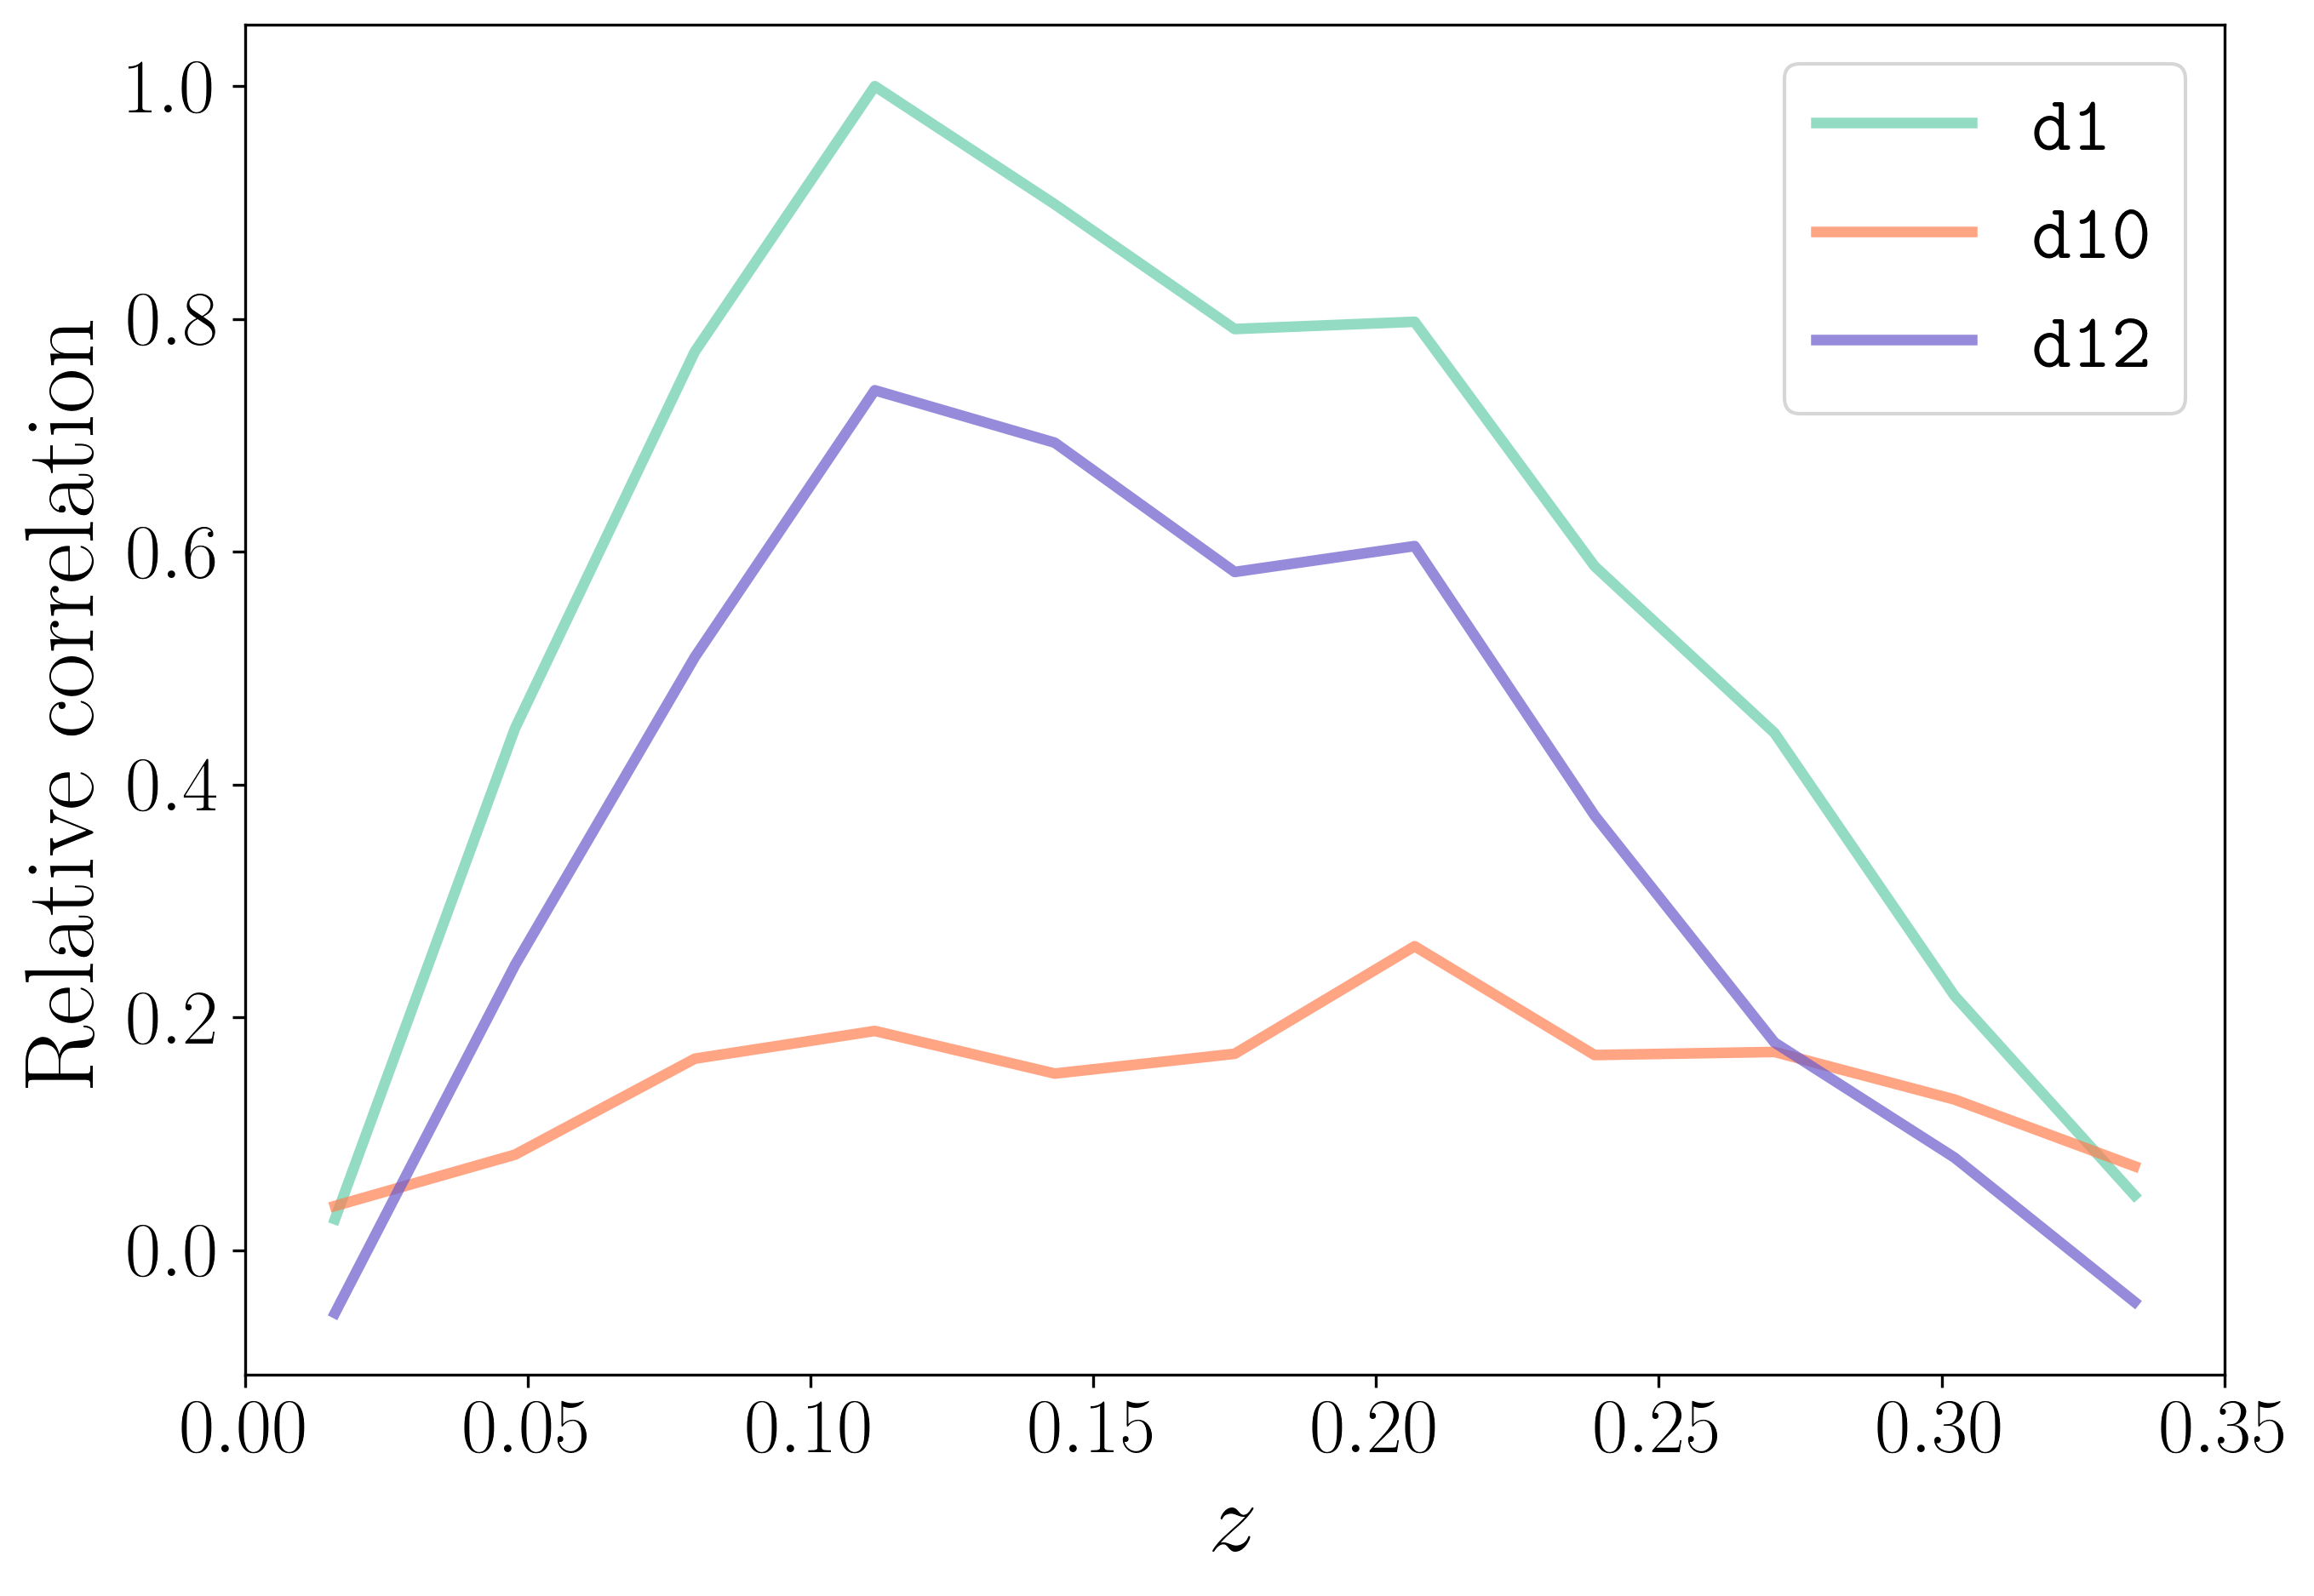
\includegraphics[width=\columnwidth]{figures/dust_galaxy_correlation.png}
    \caption{Relative extragalactic contamination in the new dust templates \texttt{d10} and \texttt{d12}, compared to the \texttt{d1} model. Contamination is quantified as the excess 857 GHz emission within $11'$ of galaxies from the GLADE+ catalog, normalized to the maximum excess and plotted as a function of redshift ($z$). The new dust templates contain less extragalactic contamination than older dust models because they are based on GNILC-processed Planck data. The improvement is most significant for \texttt{d10}. }
    \label{fig:extragal_contamination}
\end{figure}


We quantify the extragalactic contamination present in our dust models using a tomographic redshift-clustering technique \citep{Schmidt:2015, Chiang:2019}. Our intensity-based Galactic dust templates inevitably contain emission from both Galactic dust and external galaxies. As described in Section \ref{sec:dustamplitude}, the new \texttt{d9} and \texttt{d10} dust templates are derived from GNILC-processed Planck data, while older PySM dust templates used \texttt{Commander} data products. We thus expect that the new Galactic dust models are significantly less affected by CIB contamination than previous models. Here we quantify this contamination by measuring the cross-correlation between our dust models and the clustering of galaxies as a function of redshift in spectroscopic survey data. A perfect Galactic dust template would be uncorrelated with such clustering; the signature of CIB contamination is excess template emission correlated with galaxy clustering. 

Following a procedure similar to \citet{Chiang:2019}, we compute the cross-correlation between local fluctuations in the Galactic emission maps and the galaxy density as a function of redshift, using galaxies from the GLADE+ catalog \citep{Dalya:2022}. We compute this cross-correlation for each of the \texttt{d1, d10}, and \texttt{d12} dust emission templates at 857 GHz, at high Galactic latitudes (in the \texttt{GAL70} mask) within the catalog footprint. Figure \ref{fig:extragal_contamination} shows that while each of the new GNILC-based maps contain less extragalactic contamination than \texttt{d1}, the decreased contamination is more marked in \texttt{d10} than in \texttt{d12}. This is expected, as \texttt{d10} and similar templates have random small-scale structure, while \texttt{d12} retains more of the structure of the data at small scales. 

We perform the same cross-correlation analysis to quantify the extragalactic contamination in the $\beta_d$ maps. We find, as expected, higher extragalactic contamination in the \texttt{d1} $\beta_d$ map than in the \texttt{d10} $\beta_d$ map. We emphasize that the mitigation of CIB contamination in the GNILC-processed Planck data affects both the spatial structure of the template frequency maps \textit{and} their extrapolation to other frequencies via the spectral parameter maps. 

\subsection{Non-Gaussianity} \label{sec:nongaussianity}

We quantify the level of non-Gaussianity in the small-scale dust emission generated through the polarization fraction tensor transformation using the simulations from dust model \texttt{d10} at 353 GHz (which is identical to the \texttt{d9} dust at that frequency). To measure the non-Gaussianity in the maps we consider the Minkowski Functionals \citep[MFs,][]{Minkowski1903}, which are a common tool to quantify map-space higher order statistical properties \citep{Martire:2023, Carones:2024}. 
Hadwiger’s theorem \citep{hadwigerVorlesungenUeberInhalt1957}
implies that, for any $n$-dimensional excursion set defined with a threshold value $\rho$, there exist $n+1$ MFs that geometrically and topologically describe the morphology of the set. In our case, for two-dimensional maps, we have three kinds of MFs. These are $\mathcal{V}_0$, $\mathcal{V}_1$, and $\mathcal{V}_2$, which correspond to the area, the perimeter and the connectivity of the excursion set (iso-intensity contour), respectively.

We use these MFs to compare the small-scale structure in \texttt{d10} to those of two other sets of maps: (i) maps where the small-scale structures are fully Gaussian and isotropic and (ii) maps where the small-scale structures are Gaussian but anisotropic across the sky. As described Section \ref{subsec:methodology}, the small scale structures in the \texttt{d10} model are generated as a Gaussian random field in $i$, $q$, and $u$, and are multiplied by $m_i$ and $m_p$ modulation maps before they are coadded to the large-scale maps and transformed back into $I$, $Q$ and $U$. We want to understand the impact of this effective modulation on the MFs, and therefore construct a set of maps that are modulated versions of Gaussian-random-field maps. This allows us to disentangle any non-Gaussianity generated through the modulation from the potential non-Gaussianity introduced due to the polarization fraction tensor transformation.

The first set of maps contains isotropic small-scale structure. We construct the small-scale structure by generating a Gaussian random field with power-law power spectra in $TT$, $EE$, and $BB$, using power laws fit to the power spectrum of the \texttt{d10} maps on the \texttt{GAL097} mask in the multipole range $[800, 2000]$. This Gaussian random field is then high-pass filtered to remove power below $\ell_{cut} = 200$ in both total intensity and polarization, and co-added to the large-scale dust template.

For the second set of maps, we introduce a modulation in $I$, $Q$, and $U$ that mimics the effective modulation applied to $i$, $q$, and $u$ in the construction of the \texttt{d10} maps. We generate modulation maps $m_I$ and $m_P$ from $IQU$, following the same procedure as done in $iqu$ space (Eq. \ref{eq:mod_maps}-\ref{eq:mod_maps2}). We multiply the Gaussian isotropic small-scale map described above with these modulation maps, and then co-add them with the large-scale dust template. However, we want to ensure that the power spectra of modulated Gaussian small scales computed on the individual sky-fraction masks are as close as possible to the \texttt{d10} map. To achieve this, we adjust the modulation maps $m_I$ and $m_P$ by applying different multiplicative factors to non-overlapping regions of the sky. We multiply $m_I$ and $m_P$ on the \texttt{GAL40} mask by scalar factors that adjust the mean power spectrum of the modulated small-scale structure to be equal to the power spectrum of \texttt{d10} on the same mask. We repeat this process for each successively larger sky-fraction mask, applying the approximately order-unity multiplication factor to the non-overlapping sky region at each iteration. 

We thus consider three sets of maps with different small scales co-added: model \texttt{d10}, a map with purely Gaussian small-scale structure, and a map with modulated Gaussian small-scale structure. We refer to these three maps as \texttt{poltens-ss}, \texttt{Gaussian-ss}, and \texttt{Gaussian-mod-ss}, respectively. 
We apply a high-pass filter with $\ell_{min} = 200$, using a smooth function similar to Eq.~\ref{eq:filter2}, to retain only the small scales of these maps. We calculate the MFs both on the sphere and in several selected regions of the sky projected into a Cartesian projection. 


\subsubsection{Minkowski Functionals on the sphere}

Following the algorithm in \cite{Grewal:2022}, we calculate the MFs for the three $Q$ maps on the sphere, i.e., in HEALPix format, on the \texttt{GAL080} mask. We first normalize the maps by dividing each map by its standard deviation, and compute the MFs for iso-intensity contours in the range $[-3, 3]$ (Figure \ref{fig:MF:sphere}). The MFs of the corresponding $U$ maps look very similar to $Q$ maps and are not shown here.

Figure~\ref{fig:MF:sphere} shows that when averaging over a large sky area, the MFs of \texttt{Gaussian-mod-ss} and \texttt{poltens-ss} are almost identical, while the MFs of \texttt{Gaussian-ss} differ substantially. The difference in MFs between \texttt{poltens-ss} and \texttt{Gaussian-ss} indicates the existence of non-Gaussianity in \texttt{poltens-ss}, but the similarity between \texttt{poltens-ss} and \texttt{Gaussian-mod-ss} demonstrates that the non-Gaussianity in \texttt{poltens-ss} comes from the anisotropy in the maps, which originates from the modulation, rather than from the polarization fraction tensor transformation.

\begin{figure*}
    \centering
    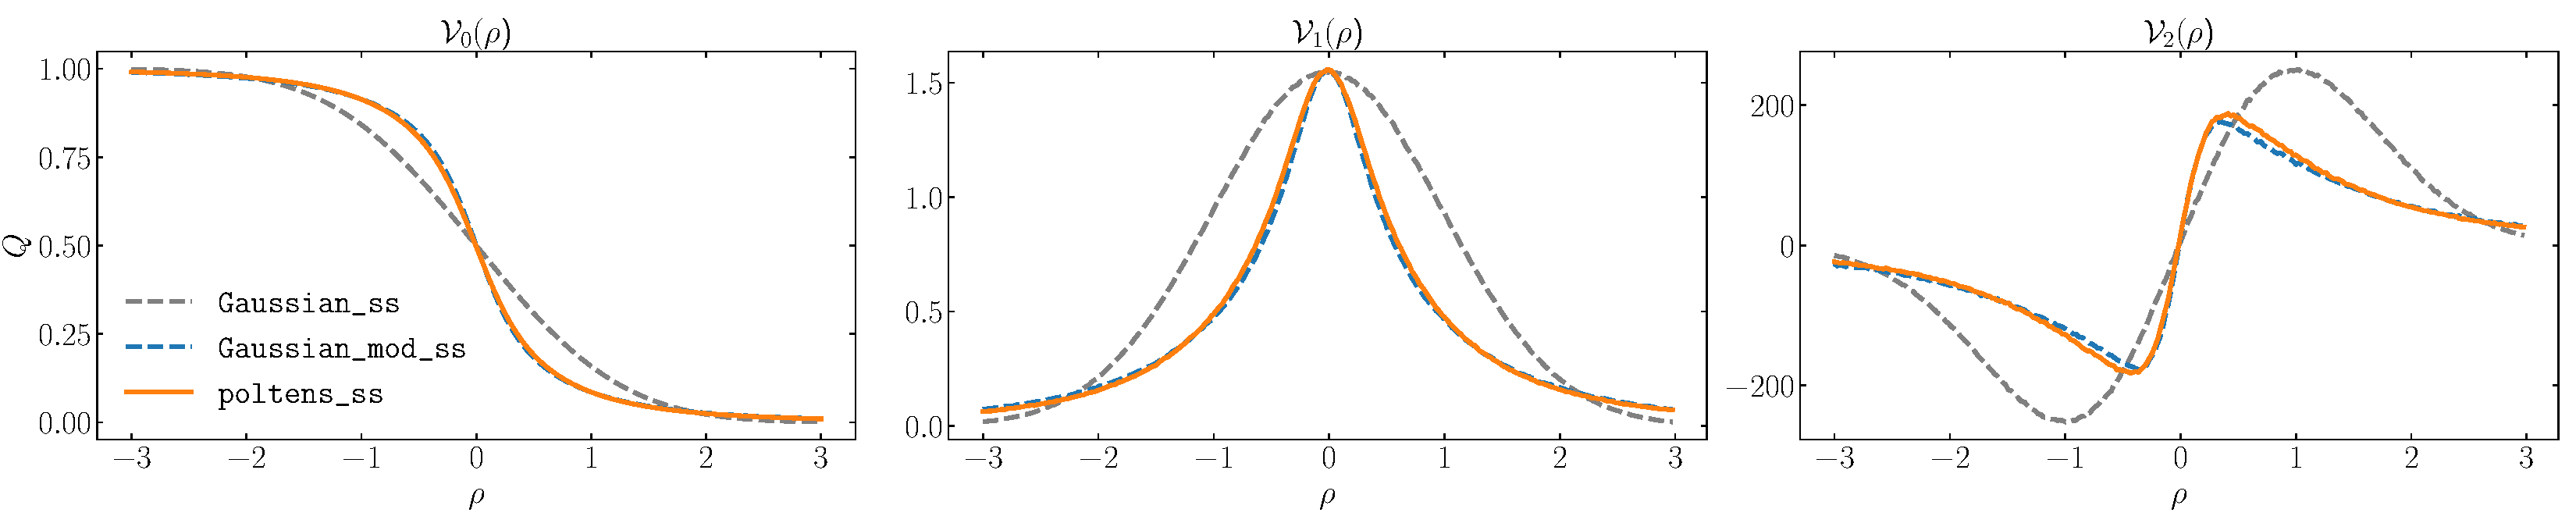
\includegraphics[width=180mm]{figures/MFs_80p_sky_Q.pdf}
    \caption{MFs for the small scales of three sets of maps on the sphere with \texttt{GAL080} mask. The large scales are filtered out by excluding multipoles $\ell < 200$ in the maps, and we choose $\ell_\text{max} = 2048$ when obtaining the small scales. We show the MFs as a function of threshold $\rho$, for \texttt{Gaussian-mod-ss} in blue, \texttt{poltens-ss} in orange and \texttt{Gaussian-ss} in dashed gray.}
    \label{fig:MF:sphere}
\end{figure*}

\begin{figure*}
    \centering
    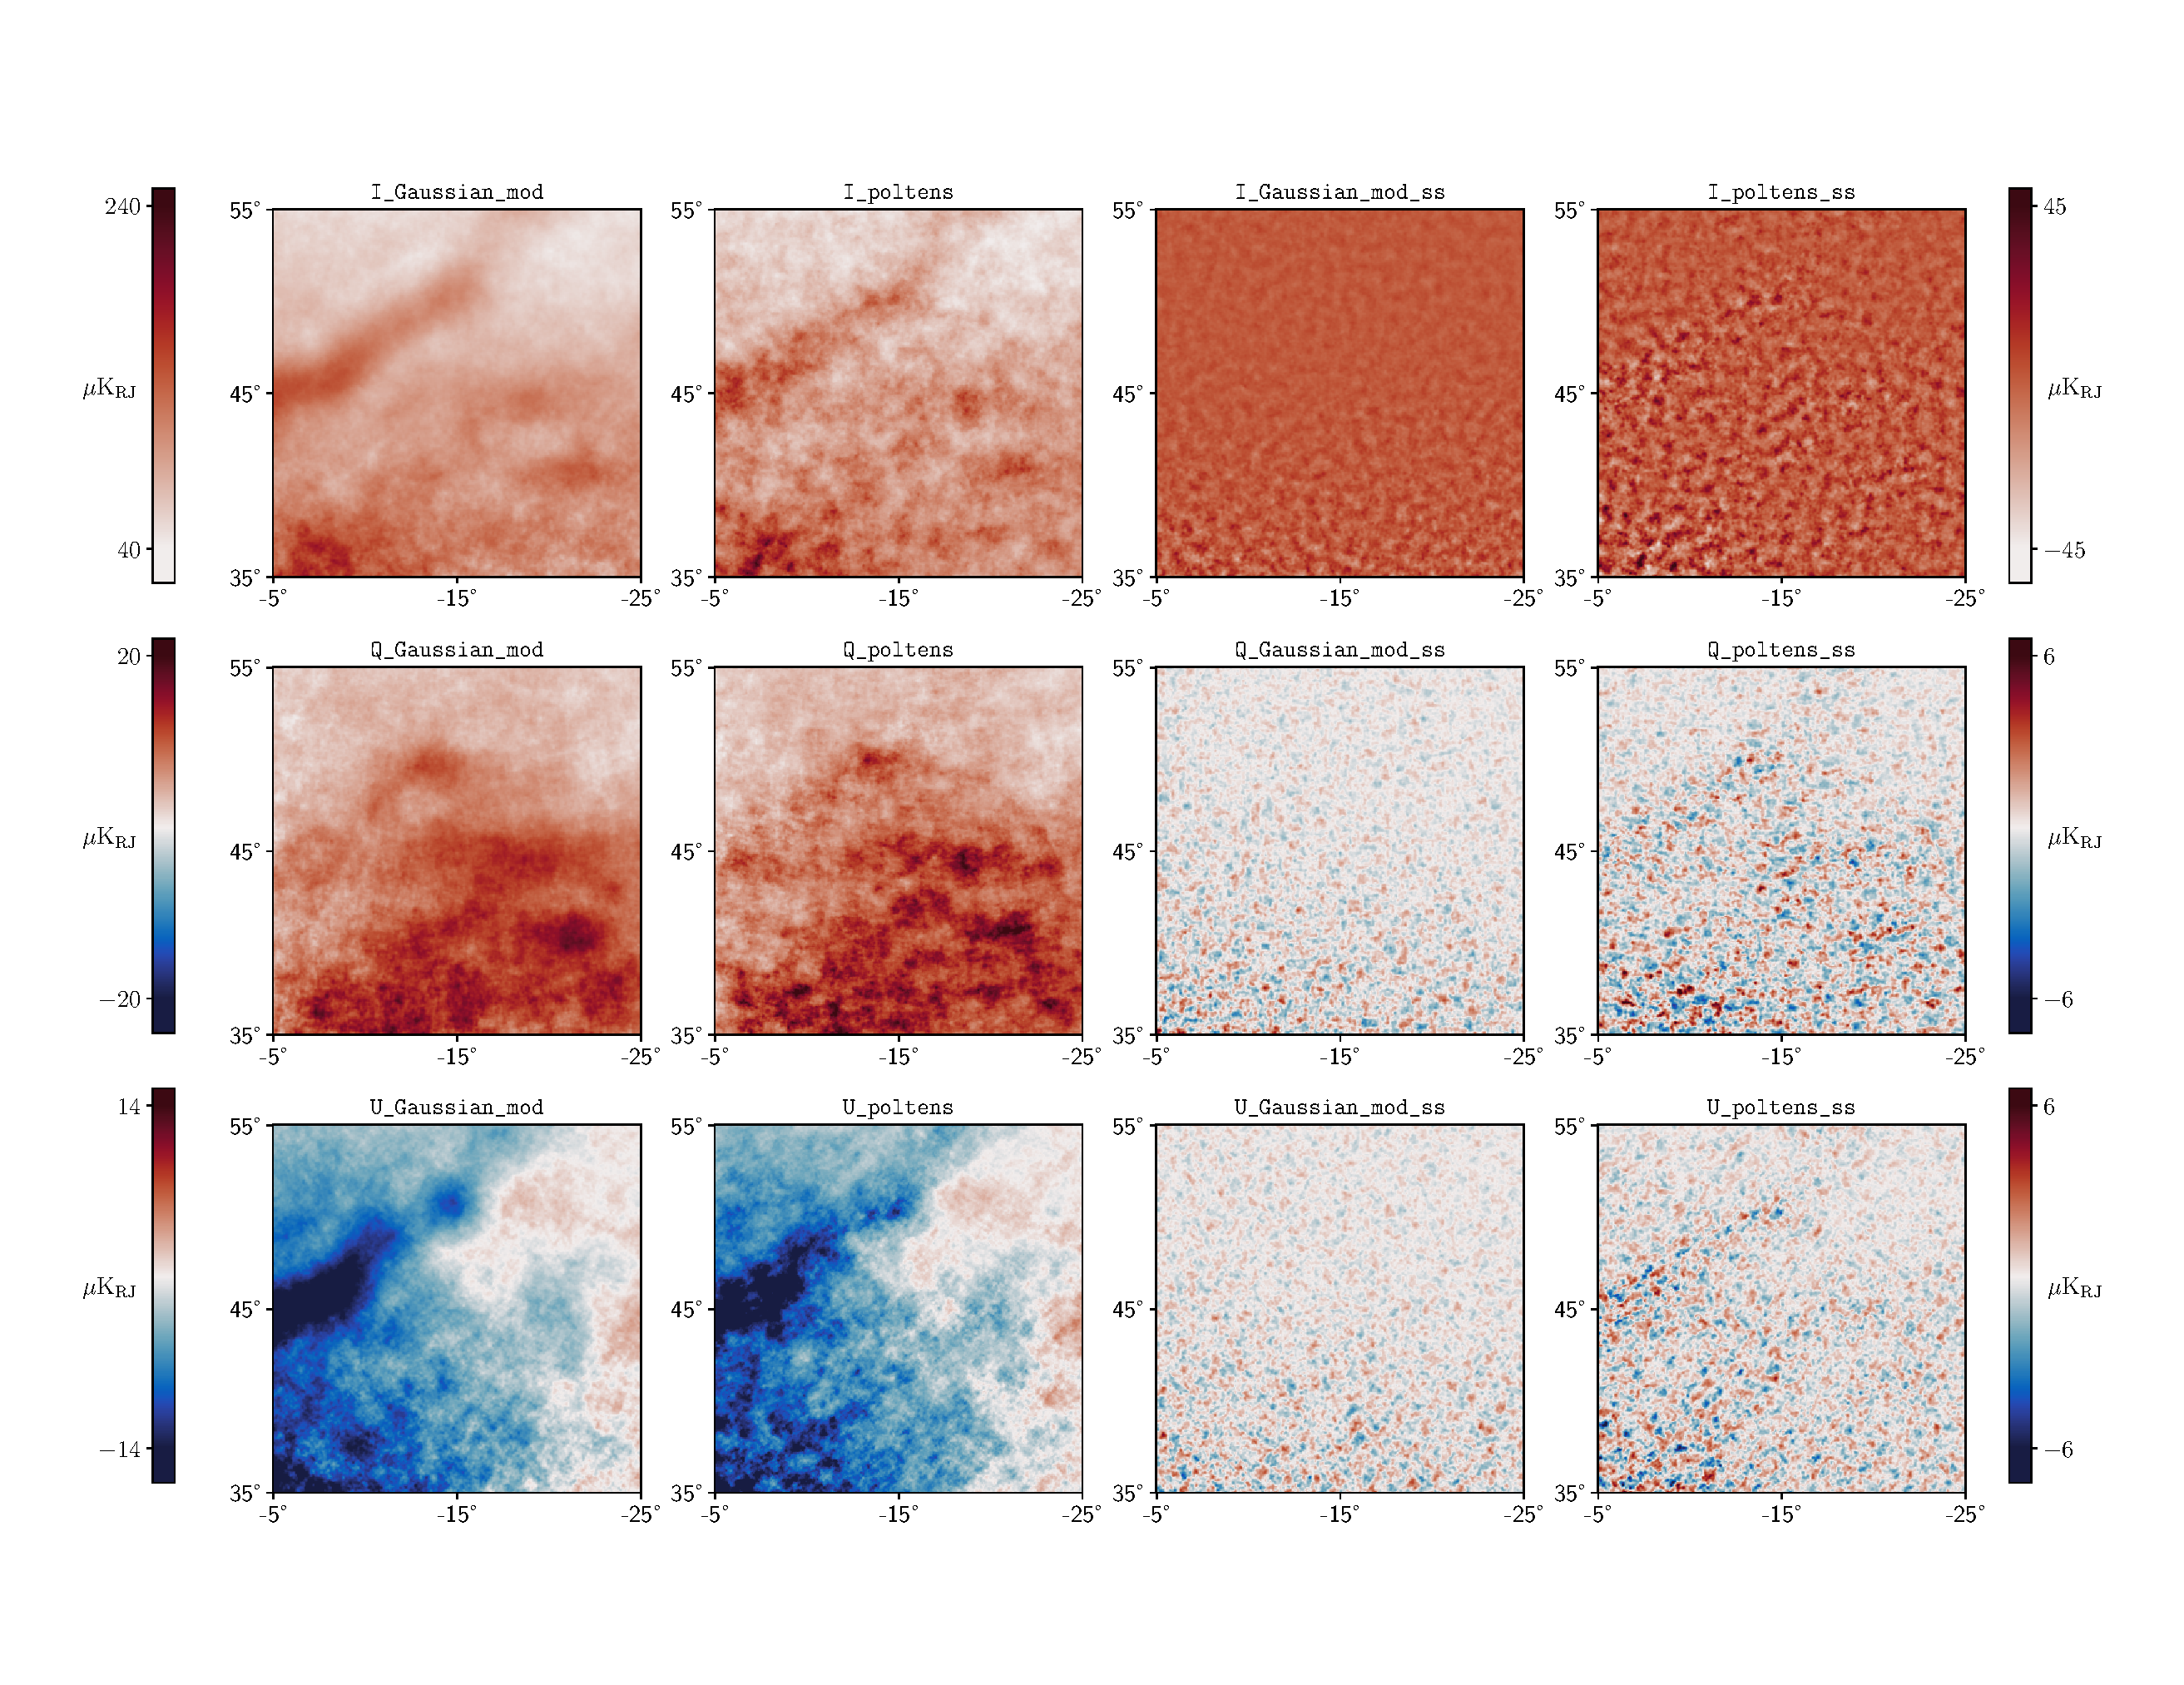
\includegraphics[width=180mm]{figures/maps_patch_345_45.pdf}
    \caption{We show the zoom-in plots in the selected patch at the center $(l, b) = (-15^{\circ}$, $45^{\circ})$, which are, from left to right, the final map with \texttt{Gaussian-mod-ss}, final map with \texttt{poltens-ss} (i.e., $\texttt{d10}$ map), \texttt{Gaussian-mod-ss} only map and \texttt{poltens-ss} only map. From top to bottom is for I, Q and U respectively. The colorbar on the left indicates the pixel values in the left-most two columns in the units of $\mu K_{RJ}$ and the colorbar on the right is for the last two columns. }
    \label{fig:maps:patch2}
\end{figure*}

\begin{figure*}
    \centering
    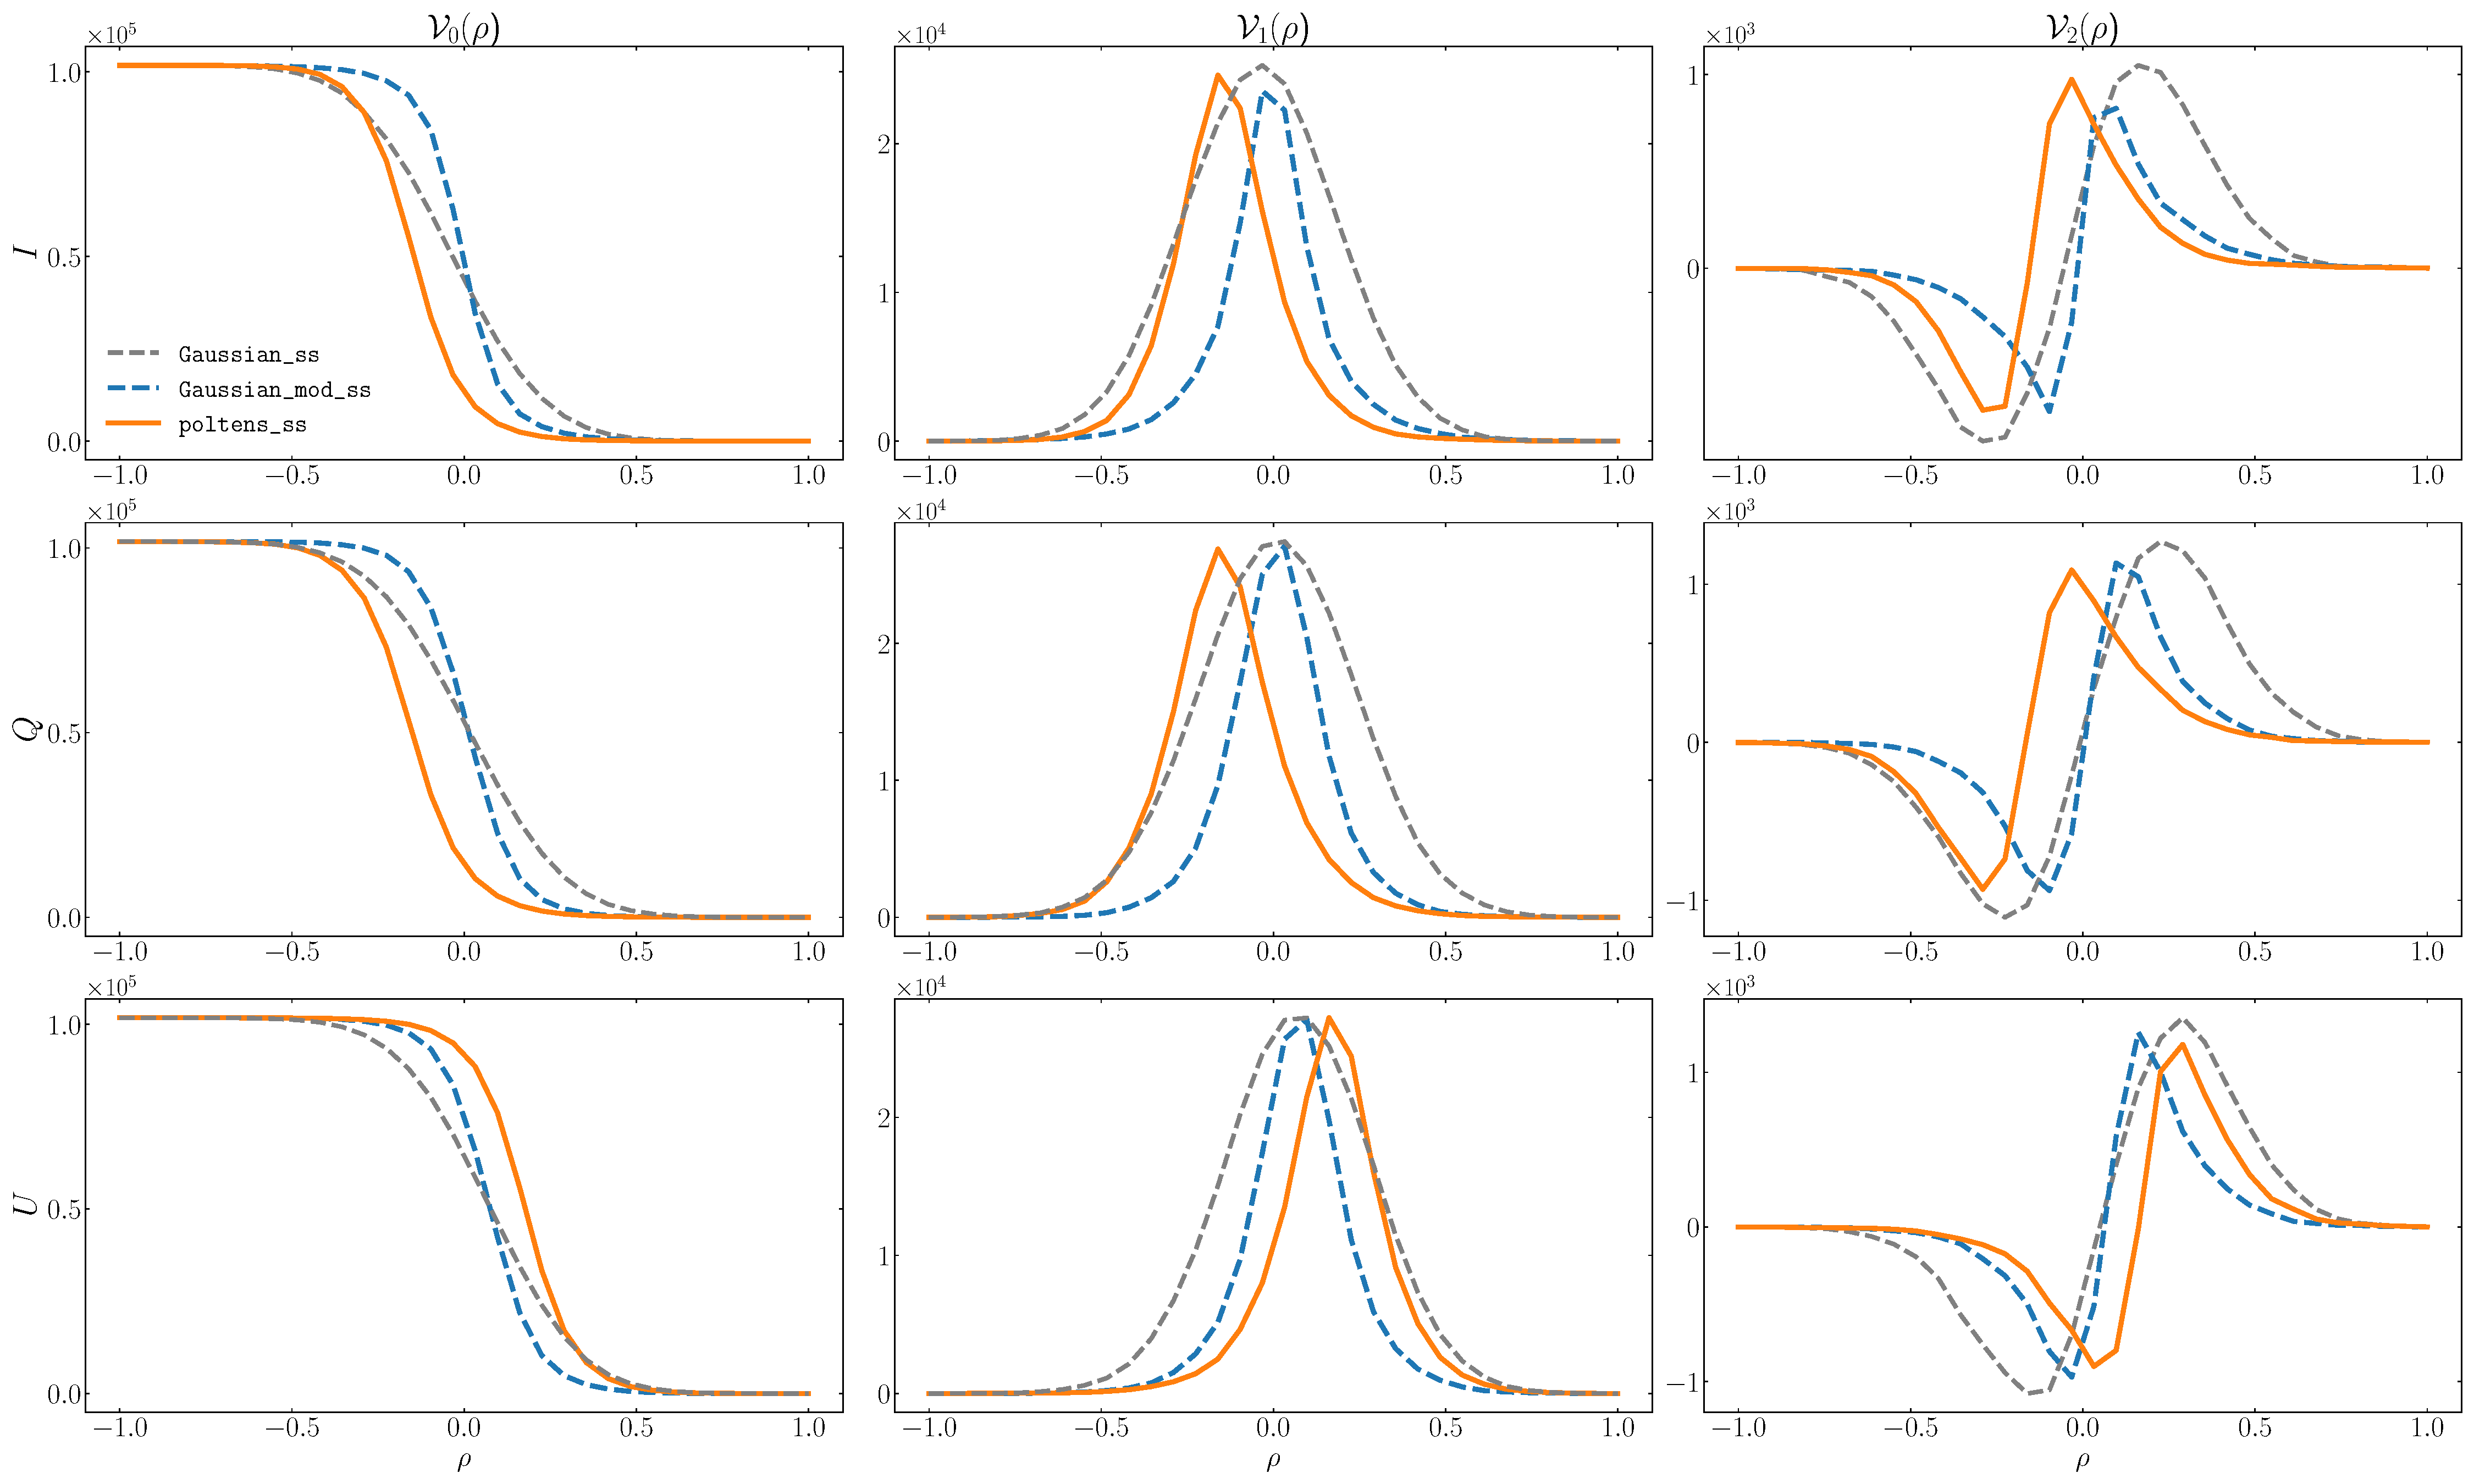
\includegraphics[width=180mm]{figures/MFs_345_45_with_G_rescaled.pdf}
    \caption{Minkowski Functionals as a function of the threshold $\rho$ for one realization of I, Q and U small scales in the patch with center of $(l, b) = (-15^{\circ}$, $45^{\circ})$ in Galactic coordinates. Each row shows three kinds of Minkowski Functionals. The blue dotted one is for \texttt{Gaussian-mod-ss} while the orange solid one is from \texttt{poltens-ss}. We also show the \texttt{Gaussian-ss} in dashed gray line as a comparison.}
    \label{fig:MF:patch2}
\end{figure*}

\subsubsection{Minkowski Functionals on small regions}
We consider a $20^{\circ}\times20^{\circ}$ region centered at $(l, b) = (-15^{\circ}$, $45^{\circ})$ to determine whether significant differences in the MFs between \texttt{Gaussian-mod-ss} and \texttt{poltens-ss} sets of maps exist in small regions of sky. Those maps are shown in Figure~\ref{fig:maps:patch2}. We can see by eye that \texttt{poltens-ss} contains structure that is not present in the \texttt{Gaussian-mod-ss} maps. We calculate the MFs of these small-scale maps, following \cite{Mantz:2008} for the calculation of MFs for a square patch. Before the calculation, we also rescale all the small scales linearly to be in the range [-1, 1], using the $minmax$ scheme.

Figure~\ref{fig:MF:patch2} shows the MFs of the \texttt{Gaussian-mod-ss} and \texttt{poltens-ss} maps presented in Figure~\ref{fig:maps:patch2}. In contrast with the large-area results presented in Figure~\ref{fig:MF:sphere}, in this case we do measure a departure of the \texttt{poltens-ss} MFs from the \texttt{Gaussian-mod-ss} ones. This means that the polarization fraction tensor transformation introduced non-Gaussian small-scale structure, distinct from pure modulation effects, that is detectable on small sky regions. We conclude that the level of induced non-Gaussianity differs from region to region and does not significantly impact the statistical properties when averaged over large sky fractions.

\section{Future Outlook} \label{sec:discussion}

The Galactic emission models presented in this work are created from the latest data from large-area surveys like Planck and are informed by the latest literature constraints on the spectral behavior of Galactic emission components. These models incorporate some of the expected complexity of polarized emission at scales that are not yet well-constrained by data---in particular, the non-Gaussianity of interstellar emission structure. While this represents a step forward in the realism of these models over previous all-sky Galactic emission models, there are a number of idealizations that could be improved in future work.

By imposing a cut-off in $\ell$ over which data-driven templates are employed, the models developed here are discarding high signal-to-noise information at small scales over portions of the sky where emission is bright. Future methodologies would ideally retain information from the templates on as small a scale as possible, with that cut-off scale varying across the sky. Further, particularly as sensitive data are being collected over partial sky areas by sensitive ground-based experiments, methods to incorporate partial sky templates should be developed.

The current models do not explicitly impose any non-zero parity-odd correlations in the polarized dust emission, i.e., the $TB$ and $EB$ correlations are zero in the power spectra that are used to extrapolate the small-scale dust emission structure. However, analysis of the Planck polarized dust emission finds a significant nonzero $TB$ correlation at $\ell \lesssim 600$ \citep{planck2016-l11A, Weiland:2020}. A proposed physical mechanism for the origin of the nonzero $TB$ signal is misalignment between dusty filaments and the projected magnetic field orientation \citep{Huffenberger:2020, Clark:2021, Cukierman:2023}: this picture also predicts the sign and amplitude of an expected nonzero $EB$ correlation. Future work could incorporate this parity-odd contribution to the polarized dust emission. Such models would be of particular use for the development of analysis techniques that seek to constrain signatures of cosmic birefringence or other parity-violating physics in the CMB \citep[e.g.,][]{Minami:2020, Eskilt:2022}.

Future work could also improve the physical realism of the small-scale emission structure. The structure of polarized dust emission on small scales is highly filamentary \citep[e.g.,][]{Clark:2015, Halal:2024}. Indeed, the diffuse ISM is generically filamentary. % Note to add citation here
Realizations of small-scale structure that have the particular character of non-Gaussianity that is realized in the sky could be generated using, for example, generative adversarial neural networks \citep{Krachmalnicoff:2021}, or scattering-transform-based techniques \citep{Regaldo-SaintBlancard:2020}.

As our knowledge of diffuse ISM physics improves, there are further opportunities for more sophisticated modeling of the Galactic emission. A recently discovered link between the mass fraction of neutral hydrogen in the cold neutral medium and the 353 GHz dust polarization fraction implies that dust polarization models could be further improved by incorporating information on the phase structure of the neutral ISM \citep{Lei:2024}. % [another example or two?]  

In addition to the small-scale structure of the diffuse dust and synchrotron emission, the real sky at these frequencies contains emission from discrete sources that are not explicitly included in our models. These include cold clumps \citep{Clancy:2023}, planetary nebulae, supernova remnants, pulsar wind nebulae \citep{Guan:2021}, and so forth. Nearby galaxies, while not technically within the scope of Galactic emission modeling, should also be incorporated as they are not included in existing simulations of the extragalactic sky.

%\giuse{The models presented in this work represent a further step forward in order to increase the complexity of Galactic emission. They  exploit the latest templates from \emph{Planck } surveys as well as latest  constraints on the spectral parameters published in the literature in the past years. This is  critical in several CMB experiments as foreground complexity  could  potentially impact  the  cosmological parameter estimates. }

%\giuse{We carefully design new foreground  models to employ a non-zero level of non-gaussianity, allowing  unprecedented analysis and studies on non-gaussian small scales Galactic residuals and their impact on the de-lensing procedure of \emph{B-}modes. }

%\giuse{The algorithms presented here can be further improved as they  currently lack of parity odd correlations, e.g.  \emph{TB} and \emph{EB}. Although sensitivity from   current experiments have prevented to detect  correlations for both estimators letting alone  a positive $TB$  correlation  at large scales \citep{planck2016-l04}, there is increasing evidence of parity violating observations \citep{Eskilt:2022, Philcox:2022} indicating  the existence of  interactions with an exotic  particle related to the Cosmic birefringence mechanism. Moreover, physical mechanism of generating non-zero correlations of dust $EB$ and $TB$ spectra have been lately proposed in the literature related to the misalignement of dust filaments with the magnetic field lines CITE Clark/Huffenberger/Cukierman .} 

\section{Recommended Model Suite}\label{sec:modelsuite}

\begin{deluxetable*}{p{0.1\textwidth} p{0.2\textwidth} p{0.5\textwidth}}
    \caption{Recommended Model Suite}
    \tablehead{\colhead{Complexity} & \colhead{Model set} & \colhead{Short description}}
    \startdata
    Low  & \texttt{d9, s4, f1, a1, co1} & Small-scale emission fluctuations in amplitude only; no frequency decorrelation in dust or synchrotron. Unpolarized CO emission.   \\
    Medium  & \texttt{d10, s5, f1, a1, co3} & Extrapolation to small scales for both amplitude and spectral parameters in dust and synchrotron. CO polarization at the 1\% level.  \\
    High  & \texttt{d12, s7, f1, a2, co3} & Dust layer model, spatially varying synchrotron curvature, polarized AME and CO.  \\
   \enddata
    \tablecomments{Summary of the suite of model sets described in Section~\ref{sec:modelsuite}. These are recommended combinations of models at three levels of complexity (low, medium, and high).}
    \label{tab:modelsuite}
\end{deluxetable*}

The models available for each emission component can be used in various combinations to form a number of unique Galactic sky models. While every user has this combinatoric freedom, we also prescribe a suite of recommended model sets. Our goal is to facilitate analyses that use a common set of assumptions. Community-wide use of this suite of Galactic emission model sets will enable easier comparisons between scientific forecasts for various experimental designs. Further, this will enable exploration of synergies between multiple experiments---for example, optimizing joint analyses of data from multiple telescopes.

Table~\ref{tab:modelsuite} details three model sets, representing increasing levels of complexity. The low complexity model set is highly idealized. Because this model implements synchrotron and dust variability in amplitude alone and not in their spectral parameters, these components exhibit no frequency decorrelation. The medium complexity model set includes Galactic emission properties that are expected physically, like sky-variable spectral parameters for the dust and synchrotron, extrapolated to small scales. The high complexity model set models Galactic emission properties that are physically realistic but as-yet undetected, like polarized AME and spatially varying synchrotron curvature. The high complexity model set uses the layer model for Galactic dust emission (Section~\ref{sec:layers}) and thus features line-of-sight frequency decorrelation, and the degree-scale decorrelation at frequencies dominated by the dust emission is near the maximum allowed by current constraints (Figure~\ref{fig:decorrelation}).

These model sets have already been executed for four experiments using the most recent bandpasses and beam models for each experiment: CMB-S4, LiteBIRD, Simons Observatory, and South Pole Telescope 3G. The results of these simulations and their documentation are publicly available in the CMB-S4 Data Portal at \url{https://data.cmb-s4.org}. The data products can be downloaded individually via direct HTTPS access as FITS files with no need of authentication, or they can be downloaded in batch mode using Globus to a Supercomputer or another Globus Endpoint.

All component models implemented in these suites are intended to be realistic over the range 1--1000\,GHz. Caution is warranted in extrapolating any model beyond this range. Most component models are valid up to $N_{\rm side}=8192$, though \texttt{d12} and the CO models have a maximum $N_{\rm side}=2048$. The legacy \texttt{f1} free-free model has known high-$\ell$ artifacts even at $N_{\rm side} = 2048$: refinement of the free-free model is planned for future work.

\section{Summary and Conclusions} \label{sec:summary}

This work presents new models of Galactic emission in total intensity and polarization at frequencies relevant to CMB experiments ($\sim$1--1000\,GHz). The key conclusions of this work as follows:

%The models represent a data-driven understanding of the processes that dominate interstellar emission at these frequencies. We characterize various properties of the models in order to compare them with each other and, where possible, validate them against observational constraints.

\begin{enumerate}
    \item We develop new models of small-scale, non-Gaussian Galactic dust and synchrotron emission based on the polarization fraction tensor framework. We combine realizations of this small-scale synthetic emission with well-measured large scales to produce maps with realistic levels of fluctuations at all angular scales, including in maps of spectral parameters (see Figure~\ref{fig:flowchart} for a schematic). The result is a set of all-sky models of dust and synchrotron emission that agree with observational data at large scales and that are consistent but stochastic at small scales.
    \item We implement the dust layer model of \citet{Martinez-Solaeche:2018} into PySM, providing an alternative dust model that has realistic line-of-sight integration, producing line-of-sight frequency decorrleation.
    \item We implement three models of CO line emission and polarization based on Planck CO maps \citep{planck2013-p03a} and on models of high-latitude CO emission from the literature \citep{Puglisi:2017}.
    \item The dust and synchrotron models implemented in this work show improved overall agreement with observational data compared to previous PySM models. In particular, the small-area dust $BB$ amplitude and ell-dependence in the power spectra of the new models align much more closely with those of the 353~GHz Planck NPIPE maps across the sky (Figure~\ref{fig:smallfield_power_all}).
    \item We demonstrate that by using dust amplitude and spectral templates derived from the GNILC algorithm, the new PySM models contain significantly less contamination from the CIB than previous models (Figure~\ref{fig:extragal_contamination}).
    \item We find that the polarization fraction tensor framework yields maps with appreciable non-Gaussian small-scale structure in small patches (Figure~\ref{fig:MF:patch2}). However, we find that the non-Gaussianity greatly diminishes when averaging over large sky areas (Figure~\ref{fig:MF:sphere}).
    \item We quantify the frequency decorrelation with the decorrelation parameter $\mathcal{R}_\ell$ (Equation~\eqref{eq:R_ell}). While all models are consistent with Planck constraints on decorrelation between 217 and 353\,GHz, they span a large range of decorrelation level and have distinct frequency dependence of $R_\ell$ (Figure~\ref{fig:decorrelation}).
    \item We define a set of three model suites denoted low, medium, and high complexity for use in CMB analyses (Table~\ref{tab:modelsuite}). The suites bracket the range of allowed dust frequency decorrelation (from none in Low Complexity to near maximal in High Complexity) and in general progress from the simplest allowed by current constraints to featuring emission components that are plausible but that have not been detected (e.g., polarized AME). 
    \item All models presented here are available in the current PySM3 release. Sky simulations using these models are available at the CMB-S4 Data Portal \url{https://data.cmb-s4.org} using the beams and bandpasses of CMB-S4, LiteBird, Simons Observatory, and South Pole Telescope 3G.
\end{enumerate}

The construction of Galactic emission simulations is necessarily an iterative process: as more data at higher sensitivity, higher angular resolution, and different frequencies become available, more well-constrained and thus more realistic simulations can be constructed. This work represents a new iteration of this ongoing effort to make CMB polarization science robust to complexities of Galactic emission in both experiment design and data analysis methods. % BH: This paragraph could be a lot better... open to suggestions

\begin{acknowledgments}

This work was supported by the National Science Foundation under grant No. AST-2106607 (PI S.E.C.). This work was carried out in part at the Jet Propulsion Laboratory, California Institute of Technology, under a contract with the National Aeronautics and Space Administration. We thank the BICEP/Keck collaboration for sharing the BK18 matrix products for the validation analysis of this paper. 

\end{acknowledgments}

\bibliography{refs, refsADS, refsPlanck}

\end{document}
